\documentclass[mscip, 12pt]{abdnthesis}
% Select one of: bsc, ma, msciip, meng, msc, mphil, phd
% Select one of 10pt, 11pt, 12pt. (BSc, MA, MScIP students must use 12pt.)
 
%% For citations, I would recommend natbib for its                          
%% flexibility, particularly when named citation styles are used, but                
%% it also has useful features for plain and those of that ilk.                      
%% The natbib package gives you the following definitons                             
%% that extend the simple \cite:                                                     
%   \citet{key} ==>>                Jones et al. (1990)                              
%   \citet*{key} ==>>               Jones, Baker, and Smith (1990)                   
%   \citep{key} ==>>                (Jones et al., 1990)                             
%   \citep*{key} ==>>               (Jones, Baker, and Smith, 1990)                  
%   \citep[chap. 2]{key} ==>>       (Jones et al., 1990, chap. 2)                    
%   \citep[e.g.][]{key} ==>>        (e.g. Jones et al., 1990)                        
%   \citep[e.g.][p. 32]{key} ==>>   (e.g. Jones et al., p. 32)                       
%   \citeauthor{key} ==>>           Jones et al.                                     
%   \citeauthor*{key} ==>>          Jones, Baker, and Smith                          
%   \citeyear{key} ==>>             1990                                             
\usepackage{parskip}
\usepackage{hyperref}
\usepackage{xcolor}
\definecolor{myLinkColor}{HTML}{0000EE}

\hypersetup{
    colorlinks=true,         % Use colored links instead of boxes
    % linkcolor={myLinkColor}, % Set this AFTER the ToC if you prefer
    citecolor={myLinkColor},     % Color for \cite links
    filecolor={magenta},     % Color for file links
    urlcolor={myLinkColor},      % Color for \url links
    linktoc=all              % Make text and page numbers in ToC clickable (optional)
}

\usepackage[round,colon,authoryear]{natbib}
\setlength{\bibsep}{0pt}
\bibliographystyle{apalike}
\usepackage{subcaption}
\usepackage[T1]{fontenc}
\usepackage{booktabs}
\usepackage{multirow}
\usepackage{amssymb}
\usepackage{siunitx}
\usepackage{float}
\usepackage{mdframed}

\usepackage{listings}

\lstdefinestyle{shell}{
    language=bash,
    basicstyle=\ttfamily\small,
    frame=single,
    breaklines=true,
    showstringspaces=false,
}


% Define the colors
\definecolor{codegreen}{rgb}{0,0.6,0}
\definecolor{codegray}{rgb}{0.5,0.5,0.5}
\definecolor{codepurple}{rgb}{0.58,0,0.82}
\definecolor{backcolour}{rgb}{0.95,0.95,0.92}

% Define the listing style
\lstdefinestyle{mystyle}{
    backgroundcolor=\color{backcolour},
    commentstyle=\color{codegreen},
    keywordstyle=\color{magenta},
    numberstyle=\tiny\color{codegray},
    stringstyle=\color{codepurple},
    basicstyle=\ttfamily\footnotesize,
    breakatwhitespace=false,
    breaklines=true,
    captionpos=b,
    keepspaces=true,
    numbers=left,
    numbersep=5pt,
    showspaces=false,
    showstringspaces=false,
    showtabs=false,
    tabsize=2
}

% Set the defined style as the default

% Define GitHub-like colors
\definecolor{ghbackground}{HTML}{F3F4F6}  % GitHub's background gray
\definecolor{ghborder}{HTML}{D1D5DB}      % GitHub's border gray
\definecolor{ghtext}{HTML}{24292E}        % GitHub's text color

% Custom inline code style
\newcommand{\inlinecode}[1]{%
    \begingroup
    \setlength{\fboxsep}{2pt}%         % Padding around text
    \setlength{\fboxrule}{0.4pt}%       % Border thickness
    \fcolorbox{ghborder}{ghbackground}{%  % Frame and background
        \texttt{\color{ghtext}#1}%        % Monospace font with text color
    }%
    \endgroup
}


\title{Evaluating Contrastive Explanations: Rolling the DiCE with AIDE}
\author{Hariss Ali Gills}
% IMO this is a bit silly, but some like to include these. To remove,
% delete this declaration and remove the option from the
% \documentclass definition above.
%\qualifications{PhD, Computer Science, University College London, 1997\\%            
%BEng (Hons.) Electrical and Electronic Engineering, The University of Wales, Swansea, 1992}
\school{Department of Computing Science}

%%%% In the final submission of a thesis, this should only be the year
%%%% of submission.  However, it is useful to use \date{\today} for drafts so that
%%%% they don't get mixed up.
    
\date{2025}

%% It is useful to split the document up as chapters and include
%% them.  LaTeX will sort out all the numbering and cross-referencing
%% for you --- if you run it enough times!

%% If you want to include only a couple of chapters then use the
%% \includeonly{} command with a list of the file/chapter names that
%% you wish to include.  NB, this must be in the preamble.

% \includeonly{introduction,faq}

\def\sfthing#1#2{\def#1{\mbox{{\small\normalfont\sffamily #2}}}}

\sfthing{\PP}{P}
\sfthing{\FF}{F}

%% This will make sure that all cross-references are correct (including
%% references to those file not included) but will produce a dvi
%% file with only those files/chapters you specify included.

\begin{document}

%%%% Create the title page and standard declaration.

\maketitle
\makedeclaration

%%%% Then the abstract and acknowledgements

\begin{abstract}
This dissertation addresses the critical need for explainability in opaque machine learning models by evaluating and comparing contrastive counterfactual explanation methods. Specifically, it investigates the performance of Diverse Counterfactual Explanations (DiCE), its genetic variant based on GeCo, and the immune-inspired Artificial Immune Diverse Explanations (AIDE) algorithm. The study employs a mixed-methods approach, combining quantitative evaluation across established metrics (including Size, Dissimilarity, Actionability, Diversity, and Runtime) with qualitative analysis using parallel coordinate plots on four standard benchmark datasets (adult, fico, compas, german\_credit). Quantitative results indicate that no single method universally outperforms others; which is in agreement with what has been reported in the literature. DiCE typically generates explanations closest to the original instance, while AIDE excels in producing diverse and actionable explanations, albeit at a higher computational cost. The genetic DiCE variant offers the fastest performance but can struggle with consistency. Using principles in Exploratory Data Analysis, parallel coordinates plots were used to visualize the counterfactuals. By going deeper, this analysis highlights differences in how methods handle feature types and how the counterfactuals align with dataset. Hence, a novel "Alignment" metric is proposed to assess the realism of generated counterfactuals relative to the data distribution of the counterfactual class, capturing the "concentration" of values. The evaluation study with the new metric concludes that the optimal choice of counterfactual explainer depends on the specific dataset. Additionally, implementations might consider employing a combination of counterfactual methods within an XAI system. Knowing that good explanations are also selective, the system should select the explanation based on the relative importance of different evaluation metrics from the end-user's perspective.

\end{abstract}

\begin{acknowledgements}
I would like to express my sincere gratitude to my supervisor, Dr. Yaji Sripada, whose guidance and expertise were invaluable throughout this project. Thank you for allowing me to explore this research area and for the insightful discussions we had.

My appreciation also extends to the lecturers and staff within the Department of Computing Science at the University of Aberdeen. The knowledge and support provided during my studies created a stimulating and enjoyable learning environment.

I am incredibly grateful to my family, Adams Ali Gills, Mehmood Riaz Gill, and Marina Gilla, for their unwavering support throughout my studies and for their help in proofreading this paper.

A special thank you also goes to my friends, Josh Shayo, Zsolt Kebel, Gergana Ivaylova, Ludovico Chiavelli,  and Klara Kramer, for their support and friendship during this long five year journey.
\end{acknowledgements}

\hypersetup{linkcolor=black}
\tableofcontents
\listoftables
\listoffigures
\hypersetup{linkcolor=myLinkColor}

\chapter{Introduction\label{chap:introduction}}
% not more than 3 pages
In recent years, Machine Learning (ML), a sub-field of Artificial Intelligence (AI), has witnessed substantial growth, leading to its increasing application in various industries to make predictions and automate processes. Although these ML models, including sophisticated deep learning architectures, have achieved remarkable success, many operate as "black boxes," making their decision-making processes opaque to human understanding. This lack of transparency poses challenges, especially when these models influence critical decisions with significant impacts on individuals' lives. Consequently, the field of eXplainable Artificial Intelligence (XAI) has emerged as a crucial research area, dedicated to developing techniques that can interpret and explain the inner workings and predictions of these black-box ML models. This report addresses the critical need for explainability in AI with counterfactual explanations, such kinds of methods offer a practical approach by identifying minimal changes to an input that would alter the model’s prediction.

\section{Motivation}
The increasing influence of ML in industrial applications, impacting major decisions with profound effects on people's lives, both positively and negatively, serves as a primary motivation for this research. When negative impacts occur, it becomes imperative for service providers and ML engineers to ensure fairness and accountability in the models \citep{arya2021ai}. Moreover, the end users need to understand the reason for a result and counterfactuals can provide useful information for all of the aforementioned parties. The European Union's General Data Protection Regulation (GDPR) has brought the concept of a "Right to Explanation" (R2Ex) for individuals affected by fully automated decisions into focus \citep{selbst2018meaningful}. This regulatory landscape underscores the urgent need for effective and automated explanation processes for AI-driven decisions. Understanding how users perceive and utilize explanations is crucial for the development of XAI systems that can enhance trust in AI.

% Talk about ricardo and AIDE
Among the approaches within XAI, counterfactual explanations stand out as a particularly intuitive, practical, and powerful method. Drawing inspiration from how humans naturally explain events. Not by detailing complex causal chains, but by contrasting what happened with a hypothetical alternative that didn't. They answer the user's implicit question, "Why this prediction instead of another?" For instance, rather than explaining every internal weight and bias of a loan application model, a counterfactual explanation might state, "You were denied because your income was too low and your credit score wasn't high enough; if your income had been \$X and your credit score Y, you would have been approved". Such explanations match with human contrastive reasoning. 

One such method is called DiCE \citep{mothilal2020explaining}, which finds a set of counterfactuals by iteratively adjusting feature values of random instances through gradient descent, aiming to find multiple alternatives that would lead to a different classification. DiCE has been evaluated and performed as well as or better than all the state of the art counterfactual methods \citep{guidotti2024counterfactual}. The \href{https://pypi.org/project/dice-ml/}{python package} that provides DiCE also has a genetic method that has not been evaluated previously. It is based on GeCo employs a customized genetic algorithm to search a defined space of plausible and feasible counterfactual explanations by iteratively applying mutation and crossover operations, leveraging optimizations for runtime performance. In contrast, AIDE introduces an innovative, immune-inspired approach derived from Artificial Immune Systems. By leveraging mechanisms akin to biological antibodies, such as cloning, mutation, and neighborhood suppression, AIDE is designed to explore multiple local optima simultaneously. This multi-modal optimization not only promotes diversity among the counterfactuals but also increases the likelihood of producing varied explanations. As a result, AIDE represents a promising alternative, in optimization-based approaches \citep{forrest2021contrastive}.

\section{Research Questions and Objectives}
% Is aide via immue properties capable of producing different kind of counterfactuals
The primary research questions driving this investigation are:
\newline
\begin{mdframed}[backgroundcolor=white,linecolor=black,linewidth=2pt]
\begin{itemize} \label{research-questions}
    \item \textbf{RQ1:} Is AIDE, an immune inspired algorithm, well suited for the task of counterfactual generation compared to DiCE? 
    \item \textbf{RQ2:} Is AIDE well suited for the task of counterfactual generation compared to the genetic variant of DiCE based on GeCo?
\end{itemize}
\end{mdframed}


\section{Project Overview}
This study describes and compares DiCE, AIDE, and genetic-DiCE. This is achieved by quantitatively assessing the performance of these explainers using metrics defined in the literature and by qualitatively evaluating their outputs using visualizations such as parallel coordinates plots that reveal underlying alignment patterns between training data and the CFs.

The experiment is written as a python package. It starts with dataset exploration and preprocessing. The package computes detailed statistics for each dataset. This step is critical for understanding the data characteristics that will influence both model training and the counterfactual explanation process. The next phase involves training the black-box classifiers. Both Random Forests, which could consist of hundreds or even thousands of individual decision trees, and Deep Neural Networks, with vast parameter spaces, are trained on these standardized tabular datasets. After model training, extensive hyperparameter tuning is performed, ensuring that each model achieves optimal performance.

After the preparatory phase is done, each method produces sets of counterfactuals based on a randomly selected instance intended to explain the prediction, with their output counterfactuals being directly compared against a comprehensive suite of quantitative metrics. Finally, the project culminates with a detailed visualization and statistical analysis step. Interactive visualizations, including parallel coordinates plots and scatterplots of the metrics, are employed to examine trends of the generated counterfactuals. These visual tools are consistent with Exploratory Data Analysis (EDA), which involves thoroughly inspecting the the data, which will help to interpret the results from the quantitative evaluations and map them to the mechanisms for each method.

\section{Project Structure}
The document is structured as follows:
\begin{itemize}
    \item \textbf{Chapter 1:} Outlines the motivation, research questions, project overview, and report structure.
    \item \textbf{Chapter 2:} Provides the background and related work in interpretable machine learning and counterfactual explanations, including the definition of desirable properties and a review of existing methods like DiCE, DiCE-genetic/GeCo, and AIDE.
    \item \textbf{Chapter 3:} Details the problem specification, including the selection of explainers for the experiment, the datasets used, and the metrics measured.
    \item \textbf{Chapter 4:} Outlines the implementation of the experiment, covering data encoding, training of black-box models, and the generation of counterfactuals with DiCE and AIDE.
    \item \textbf{Chapter 5:} Presents the results and evaluation, combining a quantitative outlook with metrics and a qualitative analysis using parallel coordinates plots.
    \item \textbf{Chapter 6:} Concludes the report with a summary of the findings and directions for future work.
    \item \textbf{Appendices:} Includes a user manual to run the experiment and a maintenance manual to modify or extend the project.
\end{itemize}
\chapter{Introduction\label{chap:introduction}}
% not more than 3 pages
In recent years, Machine Learning (ML), a sub-field of Artificial Intelligence (AI), has witnessed substantial growth, leading to its increasing application in various industries to make predictions and automate processes. Although these ML models, including sophisticated deep learning architectures, have achieved remarkable success, many operate as "black boxes," making their decision-making processes opaque to human understanding. This lack of transparency poses challenges, especially when these models influence critical decisions with significant impacts on individuals' lives. Consequently, the field of eXplainable Artificial Intelligence (XAI) has emerged as a crucial research area, dedicated to developing techniques that can interpret and explain the inner workings and predictions of these black-box ML models. This report addresses the critical need for explainability in AI with counterfactual explanations, such kinds of methods offer a practical approach by identifying minimal changes to an input that would alter the model’s prediction.

\section{Motivation}
The increasing influence of ML in industrial applications, impacting major decisions with profound effects on people's lives, both positively and negatively, serves as a primary motivation for this research. When negative impacts occur, it becomes imperative for service providers and ML engineers to ensure fairness and accountability in the models \citep{arya2021ai}. Moreover, the end users need to understand the reason for a result and counterfactuals can provide useful information for all of the aforementioned parties. The European Union's General Data Protection Regulation (GDPR) has brought the concept of a "Right to Explanation" (R2Ex) for individuals affected by fully automated decisions into focus \citep{selbst2018meaningful}. This regulatory landscape underscores the urgent need for effective and automated explanation processes for AI-driven decisions. Understanding how users perceive and utilize explanations is crucial for the development of XAI systems that can enhance trust in AI.

% Talk about ricardo and AIDE
Among the approaches within XAI, counterfactual explanations stand out as a particularly intuitive, practical, and powerful method. Drawing inspiration from how humans naturally explain events. Not by detailing complex causal chains, but by contrasting what happened with a hypothetical alternative that didn't. They answer the user's implicit question, "Why this prediction instead of another?" For instance, rather than explaining every internal weight and bias of a loan application model, a counterfactual explanation might state, "You were denied because your income was too low and your credit score wasn't high enough; if your income had been \$X and your credit score Y, you would have been approved". Such explanations match with human contrastive reasoning. 

One such method is called DiCE \citep{mothilal2020explaining}, which finds a set of counterfactuals by iteratively adjusting feature values of random instances through gradient descent, aiming to find multiple alternatives that would lead to a different classification. DiCE has been evaluated and performed as well as or better than all the state of the art counterfactual methods \citep{guidotti2024counterfactual}. The \href{https://pypi.org/project/dice-ml/}{python package} that provides DiCE also has a genetic method that has not been evaluated previously. It is based on GeCo employs a customized genetic algorithm to search a defined space of plausible and feasible counterfactual explanations by iteratively applying mutation and crossover operations, leveraging optimizations for runtime performance. In contrast, AIDE introduces an innovative, immune-inspired approach derived from Artificial Immune Systems. By leveraging mechanisms akin to biological antibodies, such as cloning, mutation, and neighborhood suppression, AIDE is designed to explore multiple local optima simultaneously. This multi-modal optimization not only promotes diversity among the counterfactuals but also increases the likelihood of producing varied explanations. As a result, AIDE represents a promising alternative, in optimization-based approaches \citep{forrest2021contrastive}.

\section{Research Questions and Objectives}
% Is aide via immue properties capable of producing different kind of counterfactuals
The primary research questions driving this investigation are:
\newline
\begin{mdframed}[backgroundcolor=white,linecolor=black,linewidth=2pt]
\begin{itemize} \label{research-questions}
    \item \textbf{RQ1:} Is AIDE, an immune inspired algorithm, well suited for the task of counterfactual generation compared to DiCE? 
    \item \textbf{RQ2:} Is AIDE well suited for the task of counterfactual generation compared to the genetic variant of DiCE based on GeCo?
\end{itemize}
\end{mdframed}


\section{Project Overview}
This study describes and compares DiCE, AIDE, and genetic-DiCE. This is achieved by quantitatively assessing the performance of these explainers using metrics defined in the literature and by qualitatively evaluating their outputs using visualizations such as parallel coordinates plots that reveal underlying alignment patterns between training data and the CFs.

The experiment is written as a python package. It starts with dataset exploration and preprocessing. The package computes detailed statistics for each dataset. This step is critical for understanding the data characteristics that will influence both model training and the counterfactual explanation process. The next phase involves training the black-box classifiers. Both Random Forests, which could consist of hundreds or even thousands of individual decision trees, and Deep Neural Networks, with vast parameter spaces, are trained on these standardized tabular datasets. After model training, extensive hyperparameter tuning is performed, ensuring that each model achieves optimal performance.

After the preparatory phase is done, each method produces sets of counterfactuals based on a randomly selected instance intended to explain the prediction, with their output counterfactuals being directly compared against a comprehensive suite of quantitative metrics. Finally, the project culminates with a detailed visualization and statistical analysis step. Interactive visualizations, including parallel coordinates plots and scatterplots of the metrics, are employed to examine trends of the generated counterfactuals. These visual tools are consistent with Exploratory Data Analysis (EDA), which involves thoroughly inspecting the the data, which will help to interpret the results from the quantitative evaluations and map them to the mechanisms for each method.

\section{Project Structure}
The document is structured as follows:
\begin{itemize}
    \item \textbf{Chapter 1:} Outlines the motivation, research questions, project overview, and report structure.
    \item \textbf{Chapter 2:} Provides the background and related work in interpretable machine learning and counterfactual explanations, including the definition of desirable properties and a review of existing methods like DiCE, DiCE-genetic/GeCo, and AIDE.
    \item \textbf{Chapter 3:} Details the problem specification, including the selection of explainers for the experiment, the datasets used, and the metrics measured.
    \item \textbf{Chapter 4:} Outlines the implementation of the experiment, covering data encoding, training of black-box models, and the generation of counterfactuals with DiCE and AIDE.
    \item \textbf{Chapter 5:} Presents the results and evaluation, combining a quantitative outlook with metrics and a qualitative analysis using parallel coordinates plots.
    \item \textbf{Chapter 6:} Concludes the report with a summary of the findings and directions for future work.
    \item \textbf{Appendices:} Includes a user manual to run the experiment and a maintenance manual to modify or extend the project.
\end{itemize}
\chapter{Background and Related Work\label{chap:background}}
%Aim for around 7-8 pages

\section{Interpretable Machine Learning}

% Describe what machine learning is
Machine Learning (ML) is defined as the field that enables computers the ability to learn using data
without being explicitly programmed \citep{mahesh2020machine}. This analytical 
method is utilized for tasks such as cancer prognosis \citep{kourou2015machine}, credit 
card fraud detection \citep{awoyemi2017credit}, and in recommender systems \citep{portugal2018use}.

\begin{figure}[h]
  \centering
  \begin{subfigure}[b]{0.45\textwidth}
    \centering
    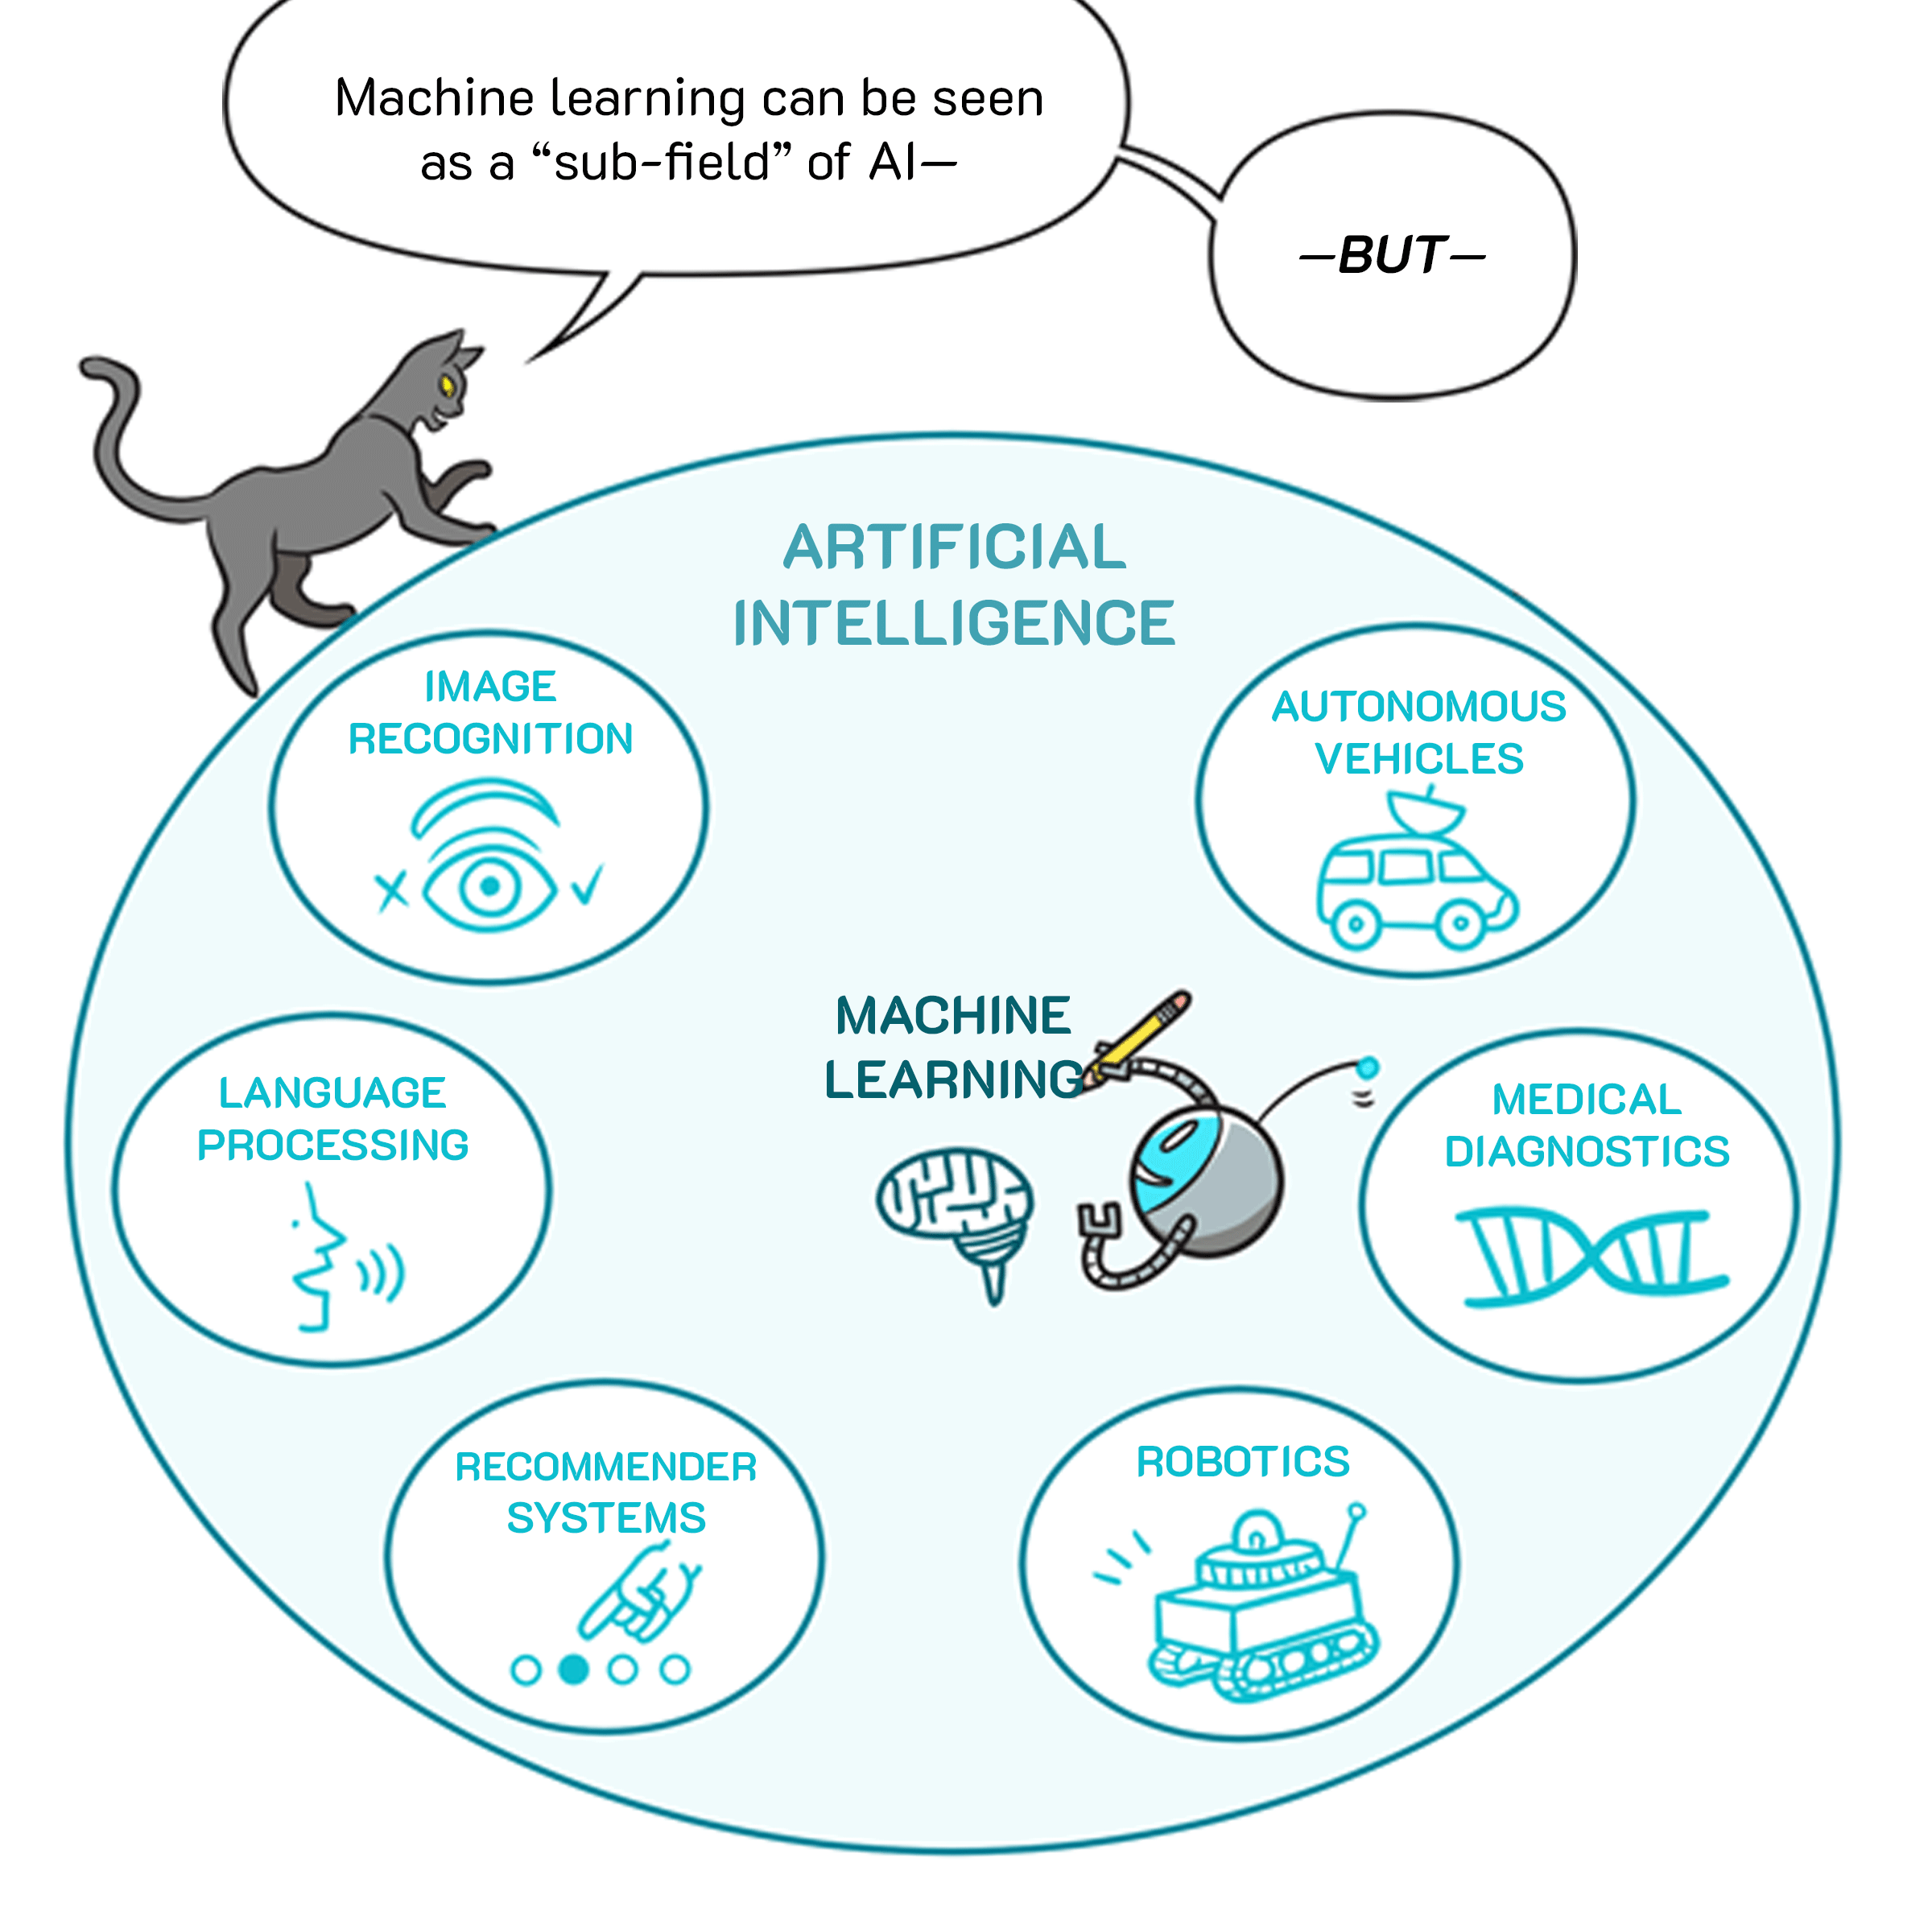
\includegraphics[width=\textwidth]{images/ml-1.png}
    \label{fig:ml-1}
  \end{subfigure}
  \hfill
  \begin{subfigure}[b]{0.45\textwidth}
    \centering
    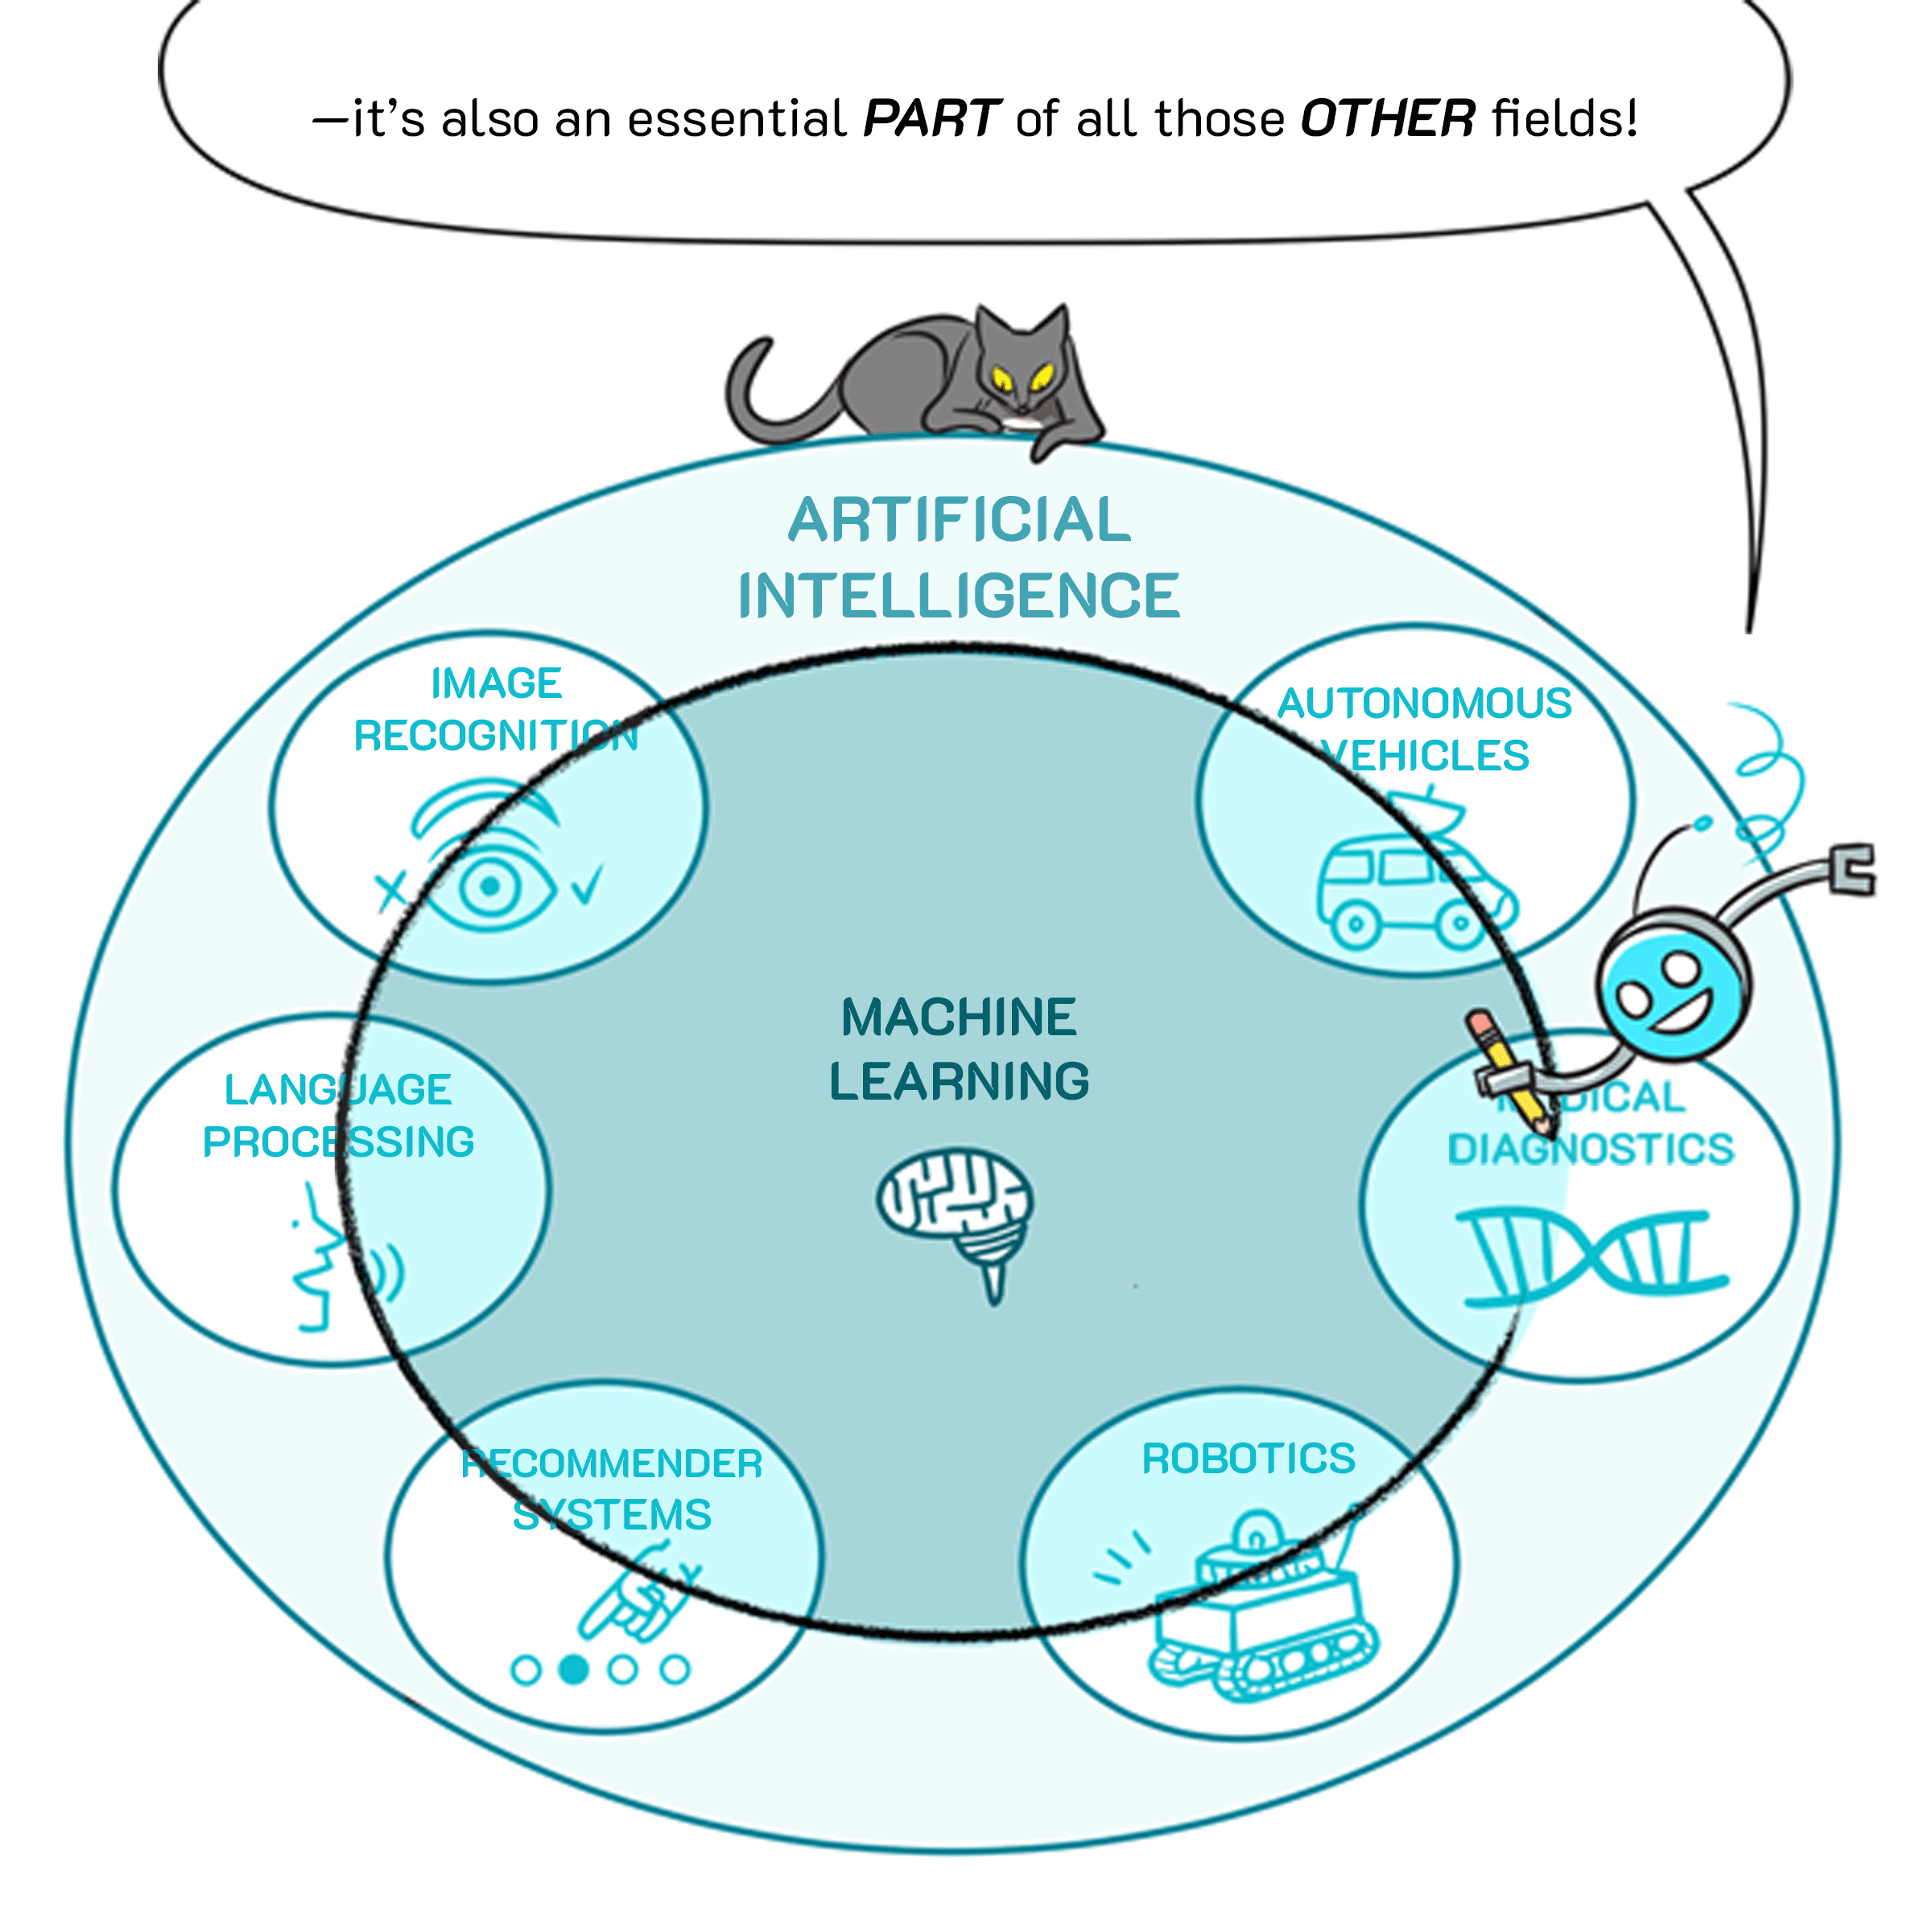
\includegraphics[width=\textwidth]{images/ml-2.png}
    \label{fig:ml-2}
  \end{subfigure}
  \caption{Images of Machine Learning in a nutshell \citep{google_comics_fact_ML}.}
  \label{fig:sidebyside}
\end{figure}

% Describe black box models
Although initial Artificial Intelligence (AI) models were more interpretable, more recently, opaque decision-making systems, notably Deep Neural Networks (DNNs), have emerged. This success in Deep Learning (DL) models is attributed to the combination of efficient learning algorithms and vast parameter spaces. These parameter spaces often include hundreds of layers and millions of individual parameters, contributing to the perception of DNNs as complex black-box models \citep{arrieta2020explainable}.

\begin{figure}[h]
  \centering
  \begin{subfigure}[b]{0.45\textwidth}
    \centering
    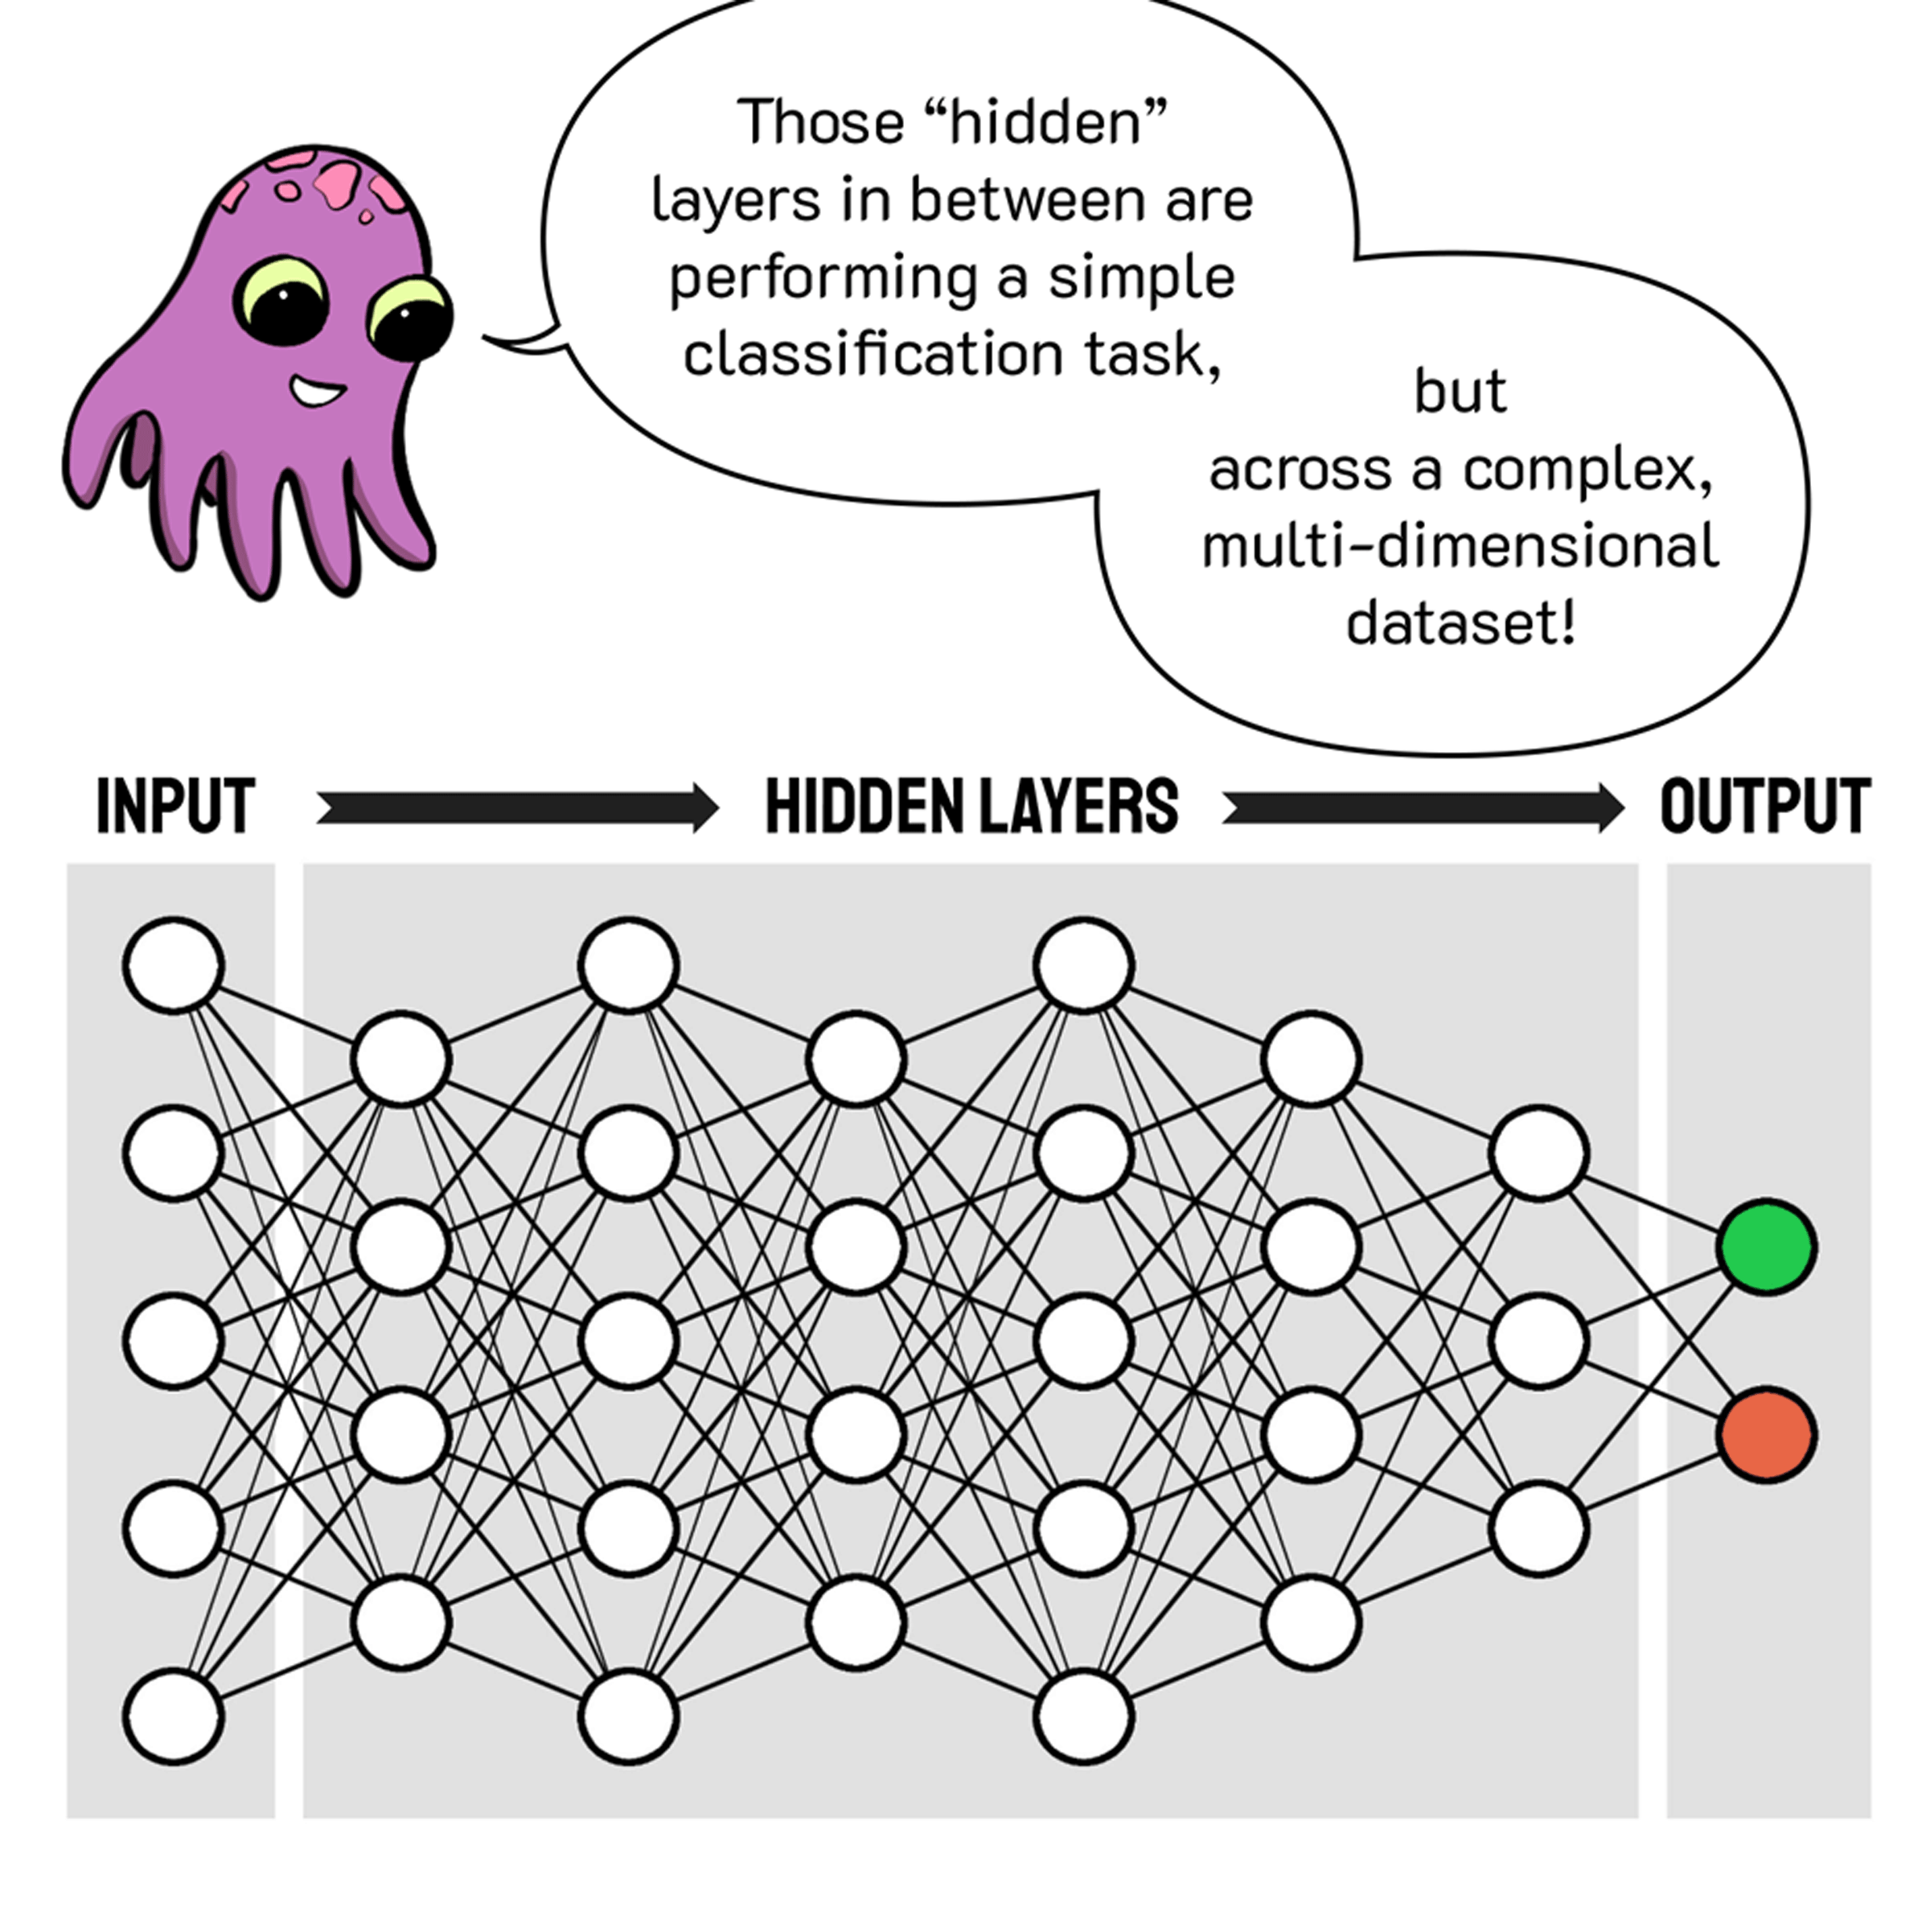
\includegraphics[width=\textwidth]{images/dnn-1.png}
    \label{fig:image1}
  \end{subfigure}
  \hfill
  \begin{subfigure}[b]{0.45\textwidth}
    \centering
    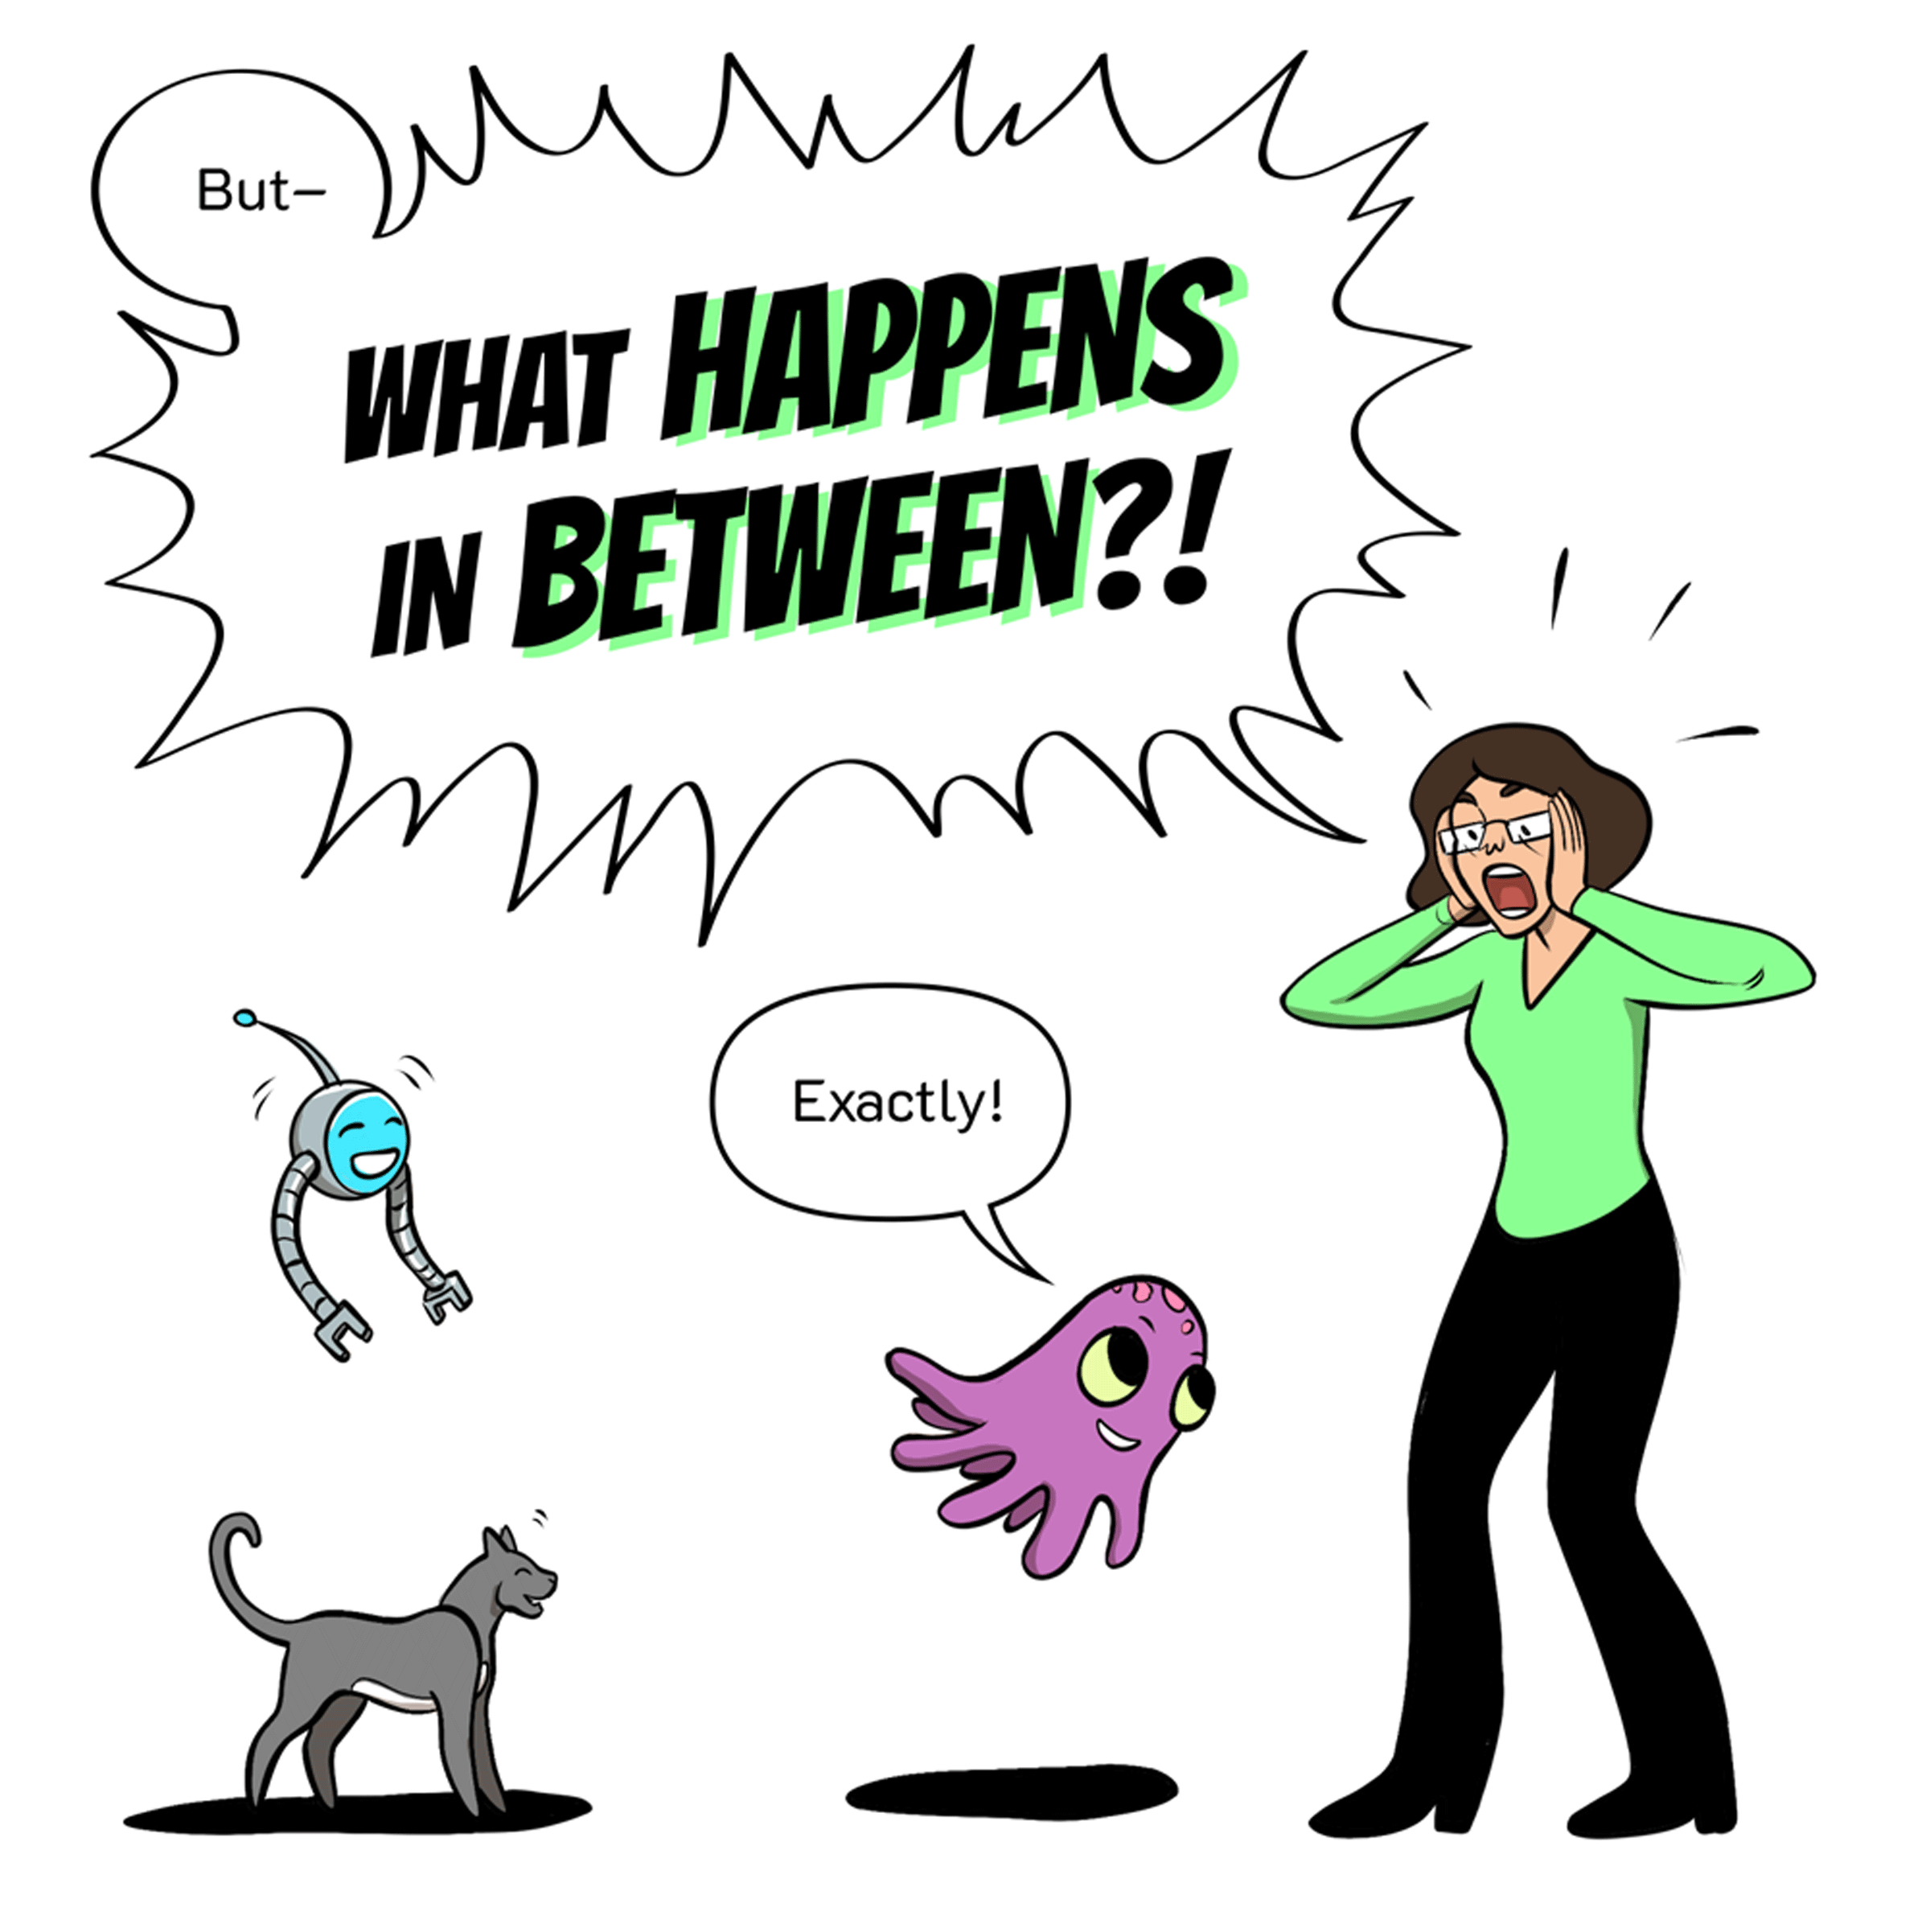
\includegraphics[width=\textwidth]{images/dnn-2.png}
    \label{fig:image2}
  \end{subfigure}
  \caption{Image of what happens in the layers of a DNN \cite{google_comics_fact_DNN}.}
  \label{fig:sidebyside}
\end{figure}
% What is Inteprteability
Hence, there has been a significant surge in eXplainable Artificial Intelligence (XAI) and interpretable machine learning \citep{goebel2018explainable}. This growing enthusiasm is reflected in the numerous books and studies that have emerged on the topic. But first, it is vital to distinguish the terminology that is related but often used interchangeably in the XAI field. There is not a clear mathematical definition for Explainability and Interpretability. However, work by \citet{arrieta2020explainable} defines the most recurring terms as follows:

\begin{itemize}
    \item \textbf{Understandability:} (or equivalently, intelligibility) Refers to a model’s inherent capacity to allow a human to grasp how it functions, without needing an explanation for internal characteristics. Concerned with both model understandability and importantly human understandability.

    \item \textbf{Comprehensibility:} Refers to a model’s ability to express what it has learned in a way that is easily understandable by humans. Into digestible units that can be directly interpreted in natural language. This idea originates from Michalski’s principles.

    \item \textbf{Interpretability:} Refers to a passive attribute that describes the extent to which a model's cause of a decision are intuitively understandable to a human observer. i.e it is concerned with the cause-and-effect relationships within the models inputs and outputs \citep{linardatos2020explainable}.
    
    \item \textbf{Explainability:} Refers to an active attribute that describes any action or procedure taken by a model with the intent of shed light on or detailing its internal functions.
    
    \item \textbf{Transparency:} A model is described as transparent if it is understandable on its own, without needing further explanation. 
\end{itemize}

% Why do we need Inteprteability Christoph Molnar
\subsection{Importance of Interpretability}
The necessity of interpretability stems from gaps in how problems are formally defined \citep{doshi2017towards}. In certain contexts, merely obtaining accurate predictions (the what) is insufficient; models must also elucidate the reasoning process behind their conclusions (the why). This is because achieving correct outputs addresses only part of the broader challenge. Understanding the logic driving these outcomes is essential to fully resolving the original problem \citep{molnar2020interpretable}. Additionally, there are other reasons that \citet{molnar2020interpretable} formalized:

\begin{itemize}
    \item \textbf{Uphold Safety:} Machine learning models are increasingly deployed in critical real-world scenarios that demand rigorous safety protocols and extensive testing. Consider, for instance, a medical diagnostic system that uses deep learning to detect tumors in imaging scans. In this case, you need absolute confidence that the system's learned abstraction is completely error-free, as even a minor mistake could lead to severe consequences for patient care. An explanation of the model's decision-making process might reveal that its primary feature is recognizing subtle irregularities in tissue patterns, which then raises important questions about edge cases, such as benign anomalies that might closely mimic the appearance of malignant tumors.
    \item \textbf{Bias Detection}: Due to their statistical nature, machine learning models tend to inherit biases present in their training data, which can lead to discriminatory behavior against underrepresented groups. Model interpretability serves as an invaluable tool for uncovering such biases. For instance, imagine you develop an automated resume screening system for hiring. Despite the goal of identifying candidates who will excel in their roles, the model might unintentionally disadvantage applicants from historically marginalized communities. The core objective is to select candidates who are likely to succeed, yet the challenge arises because the system must also ensure fairness by not discriminating based on demographics.
    \item \textbf{Social Acceptance:} Humans naturally tend to ascribe beliefs, desires, and intentions to objects around them. Now, consider an autonomous delivery robot nicknamed “Courier.” As Courier traverses busy urban sidewalks delivering packages, its actions often seem deliberate. If Courier hesitates near a construction barrier or adjusts its route unexpectedly, you might think, “Courier is intentionally avoiding obstacles to ensure a safe delivery.” Even if the full explanation behind its behavior involves multiple factors, like a low battery, sensor misalignment, or software glitches, a simple note that it encountered an obstacle can be enough to build your trust.
\end{itemize}

% other XAI methods - maybe add image here?
\subsection{XAI methods}
In the literature, XAI methods are placed into four categories. These categorize appear in \citet{guidotti2018survey}, \citet{arrieta2020explainable}, and \citet{samek2019explainable} just to a name a few. A distinguishing factor is that some methods have explainability built into the design, often called intrinsic interpretability, and those generated after the fact for black-box models, known as post-hoc interpretability. Moreover the challenge of post-hoc interpretability is further divided into model explanation, outcome explanation, and black-box inspection. Global explainers are used for model explanation, aiming to reveal the complete logic behind a model. These include partial dependence plots, which show the marginal effect one or two features have on the predicted outcome of a machine learning model \citep{friedman2001greedy} and Feature interaction (H-statistic), which quantifies to what extent the prediction is the result of joint effects of the features \citep{friedman2008predictive}. 

On the other hand, local explainers focus on outcome explanation by clarifying the reasons behind specific decisions. A method that has gained lots of popularity is Local Interpretable Model-Agnostic Explanations (LIME). It presents a specific approach to constructing these local surrogate models. Rather than developing a global surrogate to mimic the overall behavior of the black-box model, LIME emphasizes creating local surrogates that approximate the model's predictions in the vicinity of a specific instance, thereby providing insights into individual prediction outcomes \citep{ribeiro2016should}. A more widely used method is SHapley Additive exPlanations (SHAP). In this method a prediction can be interpreted by considering each feature of the instance as a "player" in a game, where the prediction represents the total reward. The Shapley value, derived from cooperative game theory, provides a fair method to allocate this reward among the features \citep{lundberg2017unified}. Lastly, these methods or also differentiated on being model-specific or model-agnostic. This based on whether a method is tailored to a specific black-box model or is sufficiently flexible to be applied across various models.

\begin{figure}[h]
    \centering
    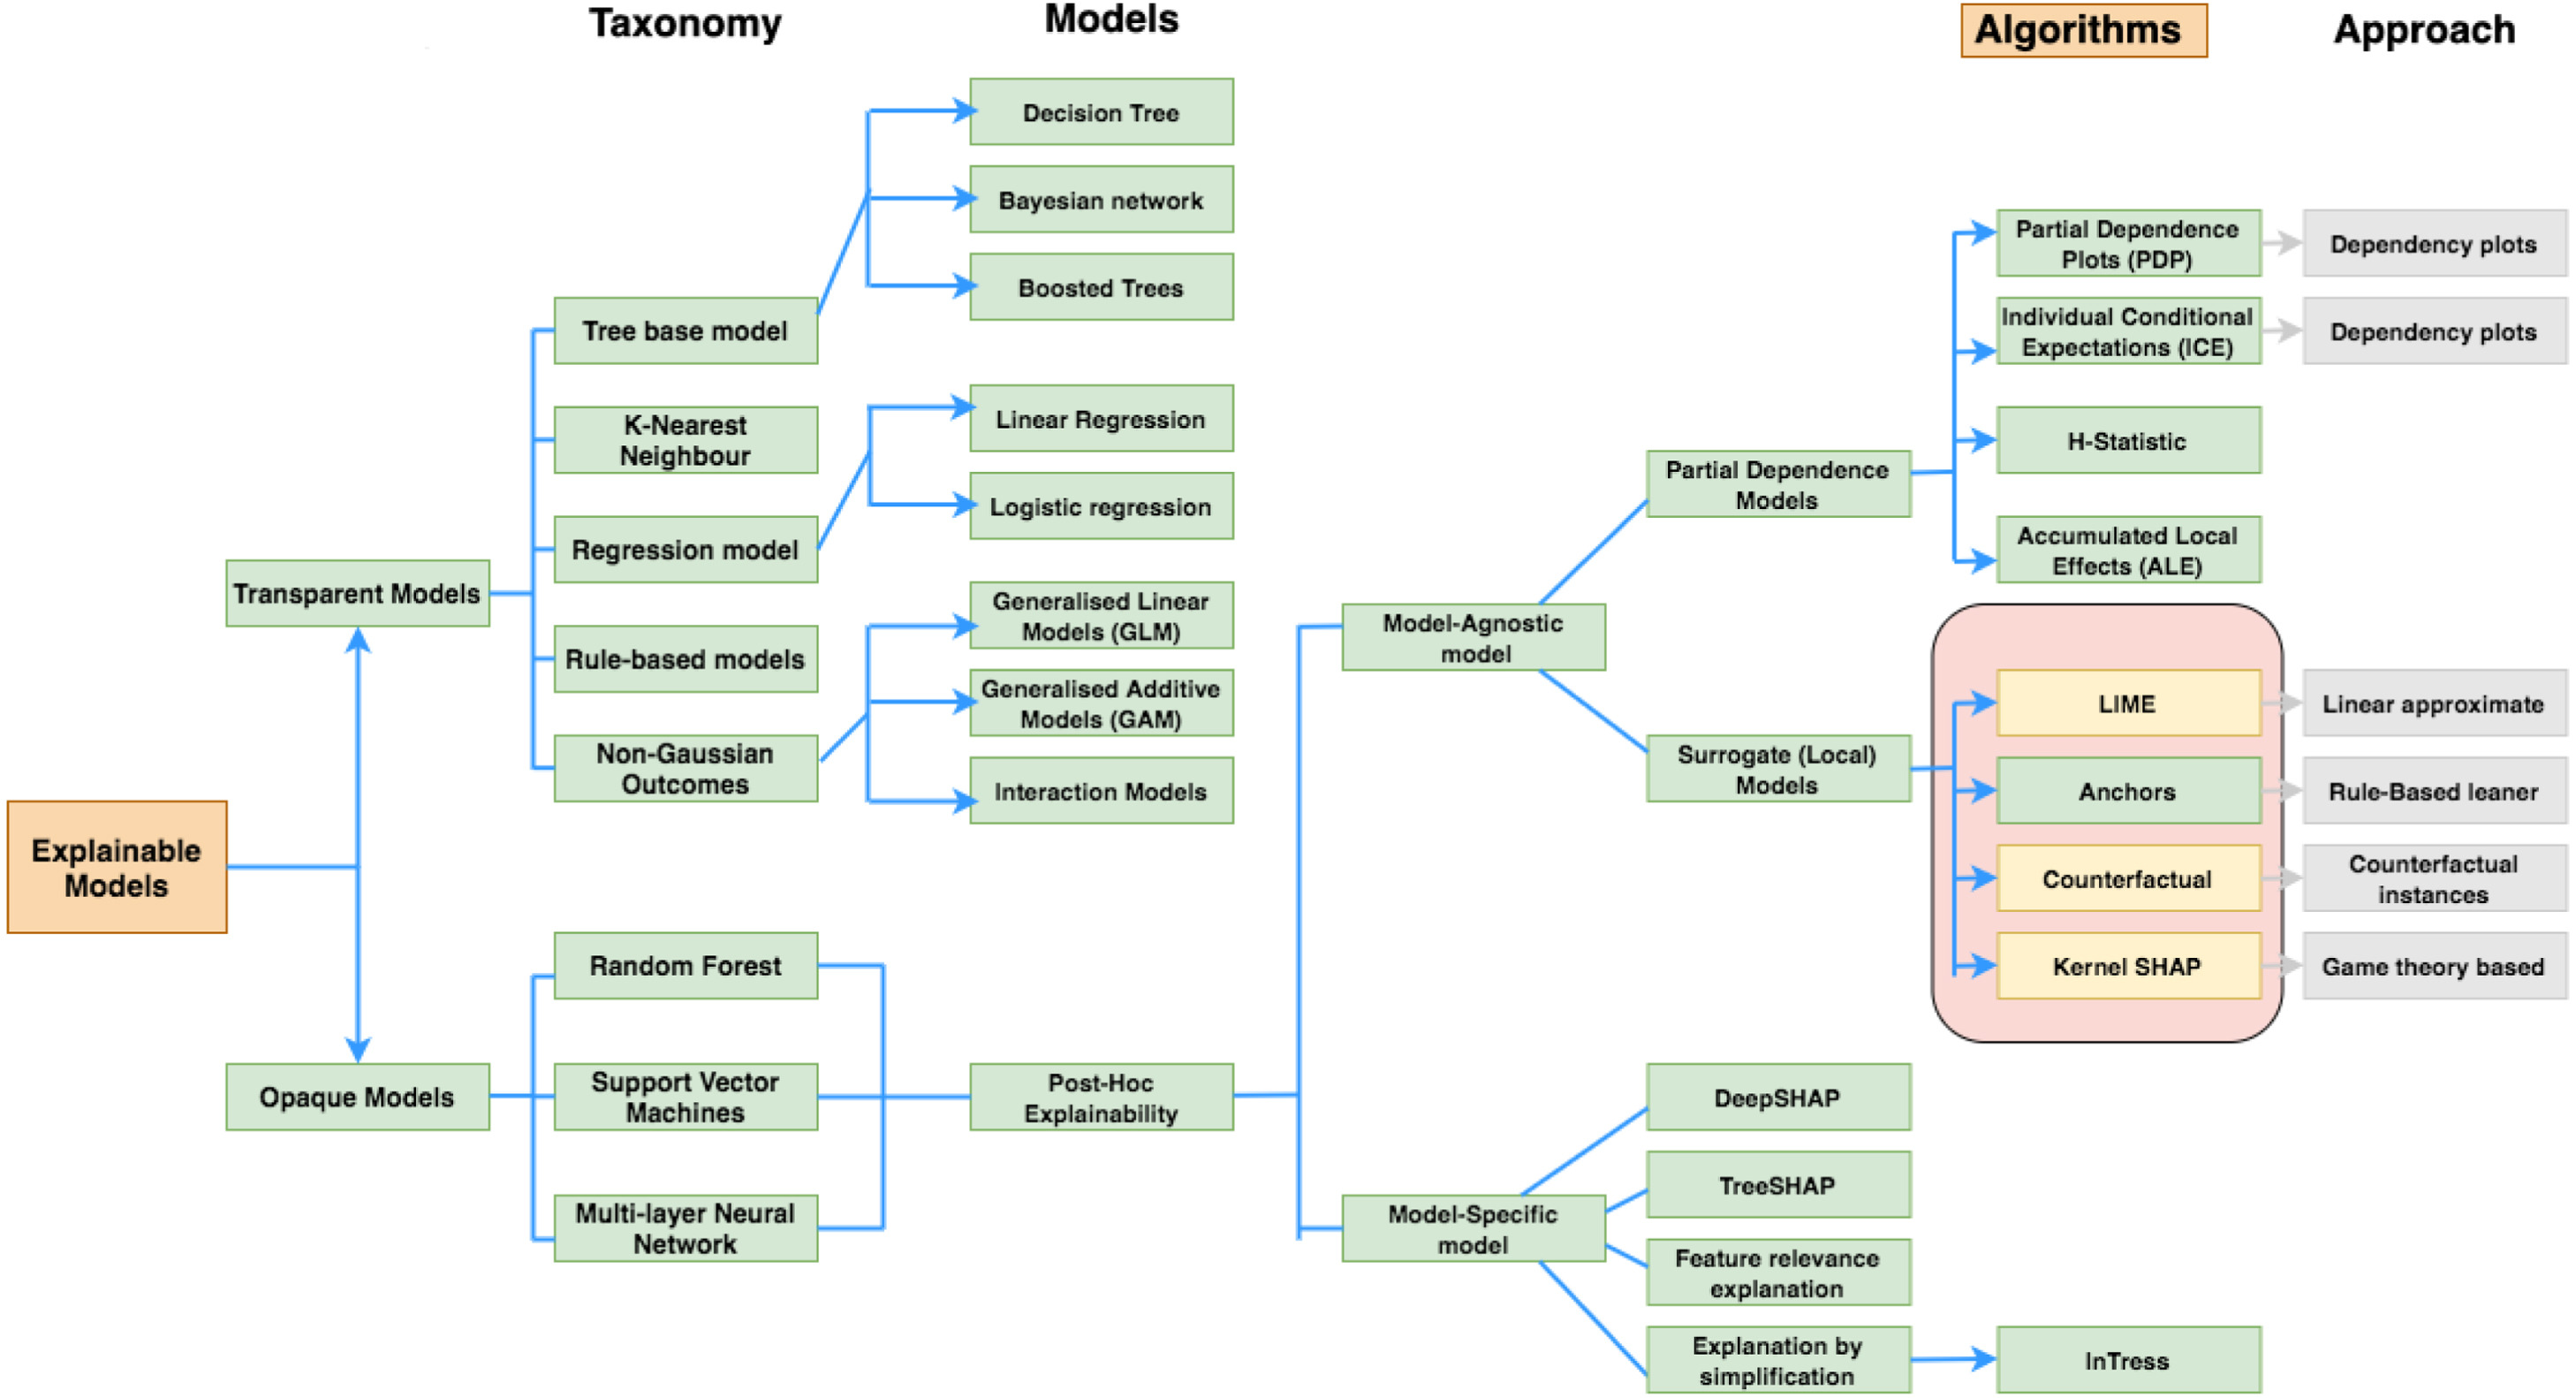
\includegraphics[width=1\textwidth]{images/taxonomy-xai.jpg}
    \caption{Image of the taxonomy of XAI methods \cite{chou2022counterfactuals}.}
    \label{fig:tax-xai}
\end{figure}

% Describe coiunterfactuals
Counterfactuals (CF) explanations suggest what should be different in the input instance to flip the outcome. This in turn, leads to a Contrastive explanation, focusing on the differences in features that led to the different outcome. As per the terminology above, Counterfactual explanations are considered post-hoc local interpretability methods. These could be model-specific or model-agnostic \citep{guidotti2024counterfactual}.


\section{Why Counterfactuals?}
% Expand on what they are clearly defined them and give examples
Work in cognitive science literature shows that individuals do not explain the cause 
of an event directly, but explain the causes comparatively to some other event that did not
occur. Additionally, this usually occurs usually implicitly. Similarly, to a multiple choice test one would ask
themselves "Why option A instead of B?". In the context of XAI, the “cause” are the specific feature values of
the input instance and the “effect” is the predicted outcome. To formalize this,
A is the target event (query instance) and B is a hypothetical counterfactual case that is hypothetical \citep{miller2019explanation}. 
As previously mentioned, B is a hypothetical because counterfactual explanations are post-hoc explainations. 
These alternative options are also usually inferred from the pragmatics of natural language.
Other terms, defined by \citet{lipton1990contrastive}, are known as "fact", the event that happened, and the "foil", the event that did not. Pearl’s interpretability scale places the foils
at the highest level of Pearl’s interpretability scale \citep{pearl2009causal}. 
Miller et al's work also concluded that good explanations, in addition to being contrastive,
are selected in a biased manner and that they are socially aligned \citep{miller2019explanation}.
%[This can be improved]

 \begin{figure}[h]
    \centering
    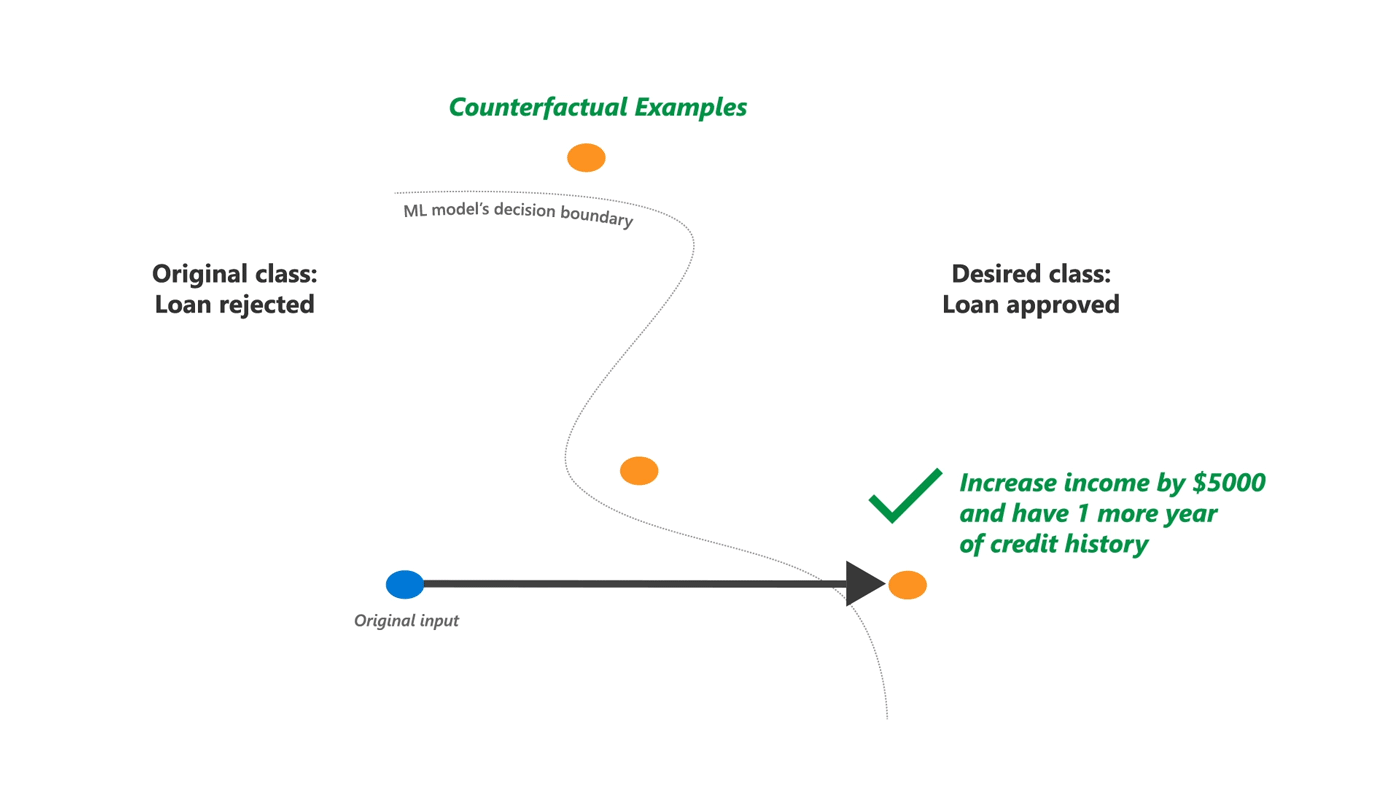
\includegraphics[width=1\textwidth]{images/counterfactual.png}
    \caption{Image of counterfactual explanations (in orange) in the loan approval dataset. As depicted in the diagram, these instances are positioned beyond the decision boundary with an explanation as to what push them to the alternative class \cite{dice_docs}.}
    \label{fig:tax-xai}
\end{figure}

 %“Why did Zsolt choose JavaScript for his dissertation?” There are many, potentially infinite, contrasts one might consider; for example, “Why did Zsolt choose JavaScript rather than opting for Python?”, “Why did he choose JavaScript instead of Java?”, or even “Why did Zsolt pick JavaScript rather than focusing on web frameworks?” Each alternative comparison invites a distinct explanation, and no single contrast is inherently assumed to be the intended foil

%Pragmatics
%Relevance to user

% Add mathematical exp?
Moreover, \citet{guidotti2024counterfactual} formalized the following mathematical definitions:

\begin{itemize}
    \item \textbf{Counterfactual Explanation}: Given a Black Box classifier $b$ that outputs the decision $y = b(x)$ for an instance $x$. A counterfactual explanation C, can be composed by a single counterfactual example $C = \{x'\}$, or by a set of counterfactual examples $C = \{x'_1, . . . , x'_h \}$ which consists of an instances $x'$ such that the decision for $b$ on $x'$ is different from $y$, i.e., 
\[
b(x') \neq y
\]
and such that the difference between $x$ and $x'$ is minimal.

\item \textbf{Counterfactual Explainer}: Is a function $f_k$ that takes as input a Black Box classifier $b$, a set $X$ of known instances, and a given instance of
interest $x$, and with its application

\[
C = f_k(x, b, X)
\]

returns a set $C = \{x'_1, . . . , x'_h \}$ of $h\leq k$ of valid counterfactual examples where $k$ is the number of counterfactuals required.
\end{itemize}

% Should I list good properties? -> I think so
\subsection{Desirable Properties of Counterfactual Explanations \label{subsection:properties}}
Counterfactual explainers have mostly aimed at tackling the task of identifying and satisfying a set of advantageous criteria. To describe the properties we will use the example "Zsolt applies for a visa and is rejected".
In this section, the beneficial attributes as described by \citet{guidotti2024counterfactual} and \citet{verma2024counterfactual}:

\begin{itemize}
    \item \textbf{Validity:} A counterfactual is valid if it actually changes the decision outcome. This ensures the definition holds. In other words, the new changed instance of Zsolt's application must be accepted.
    \item \textbf{Minimality:} (or Sparsity) The counterfactual should change as few features as possible. If there’s another counterfactual that alters fewer features than $x'$, then $x'$ isn’t considered minimal. Instead of suggesting a large overhaul of his application, the explanation might reveal that just adding one missing document enough.
    \item \textbf{Similarity:} (or Proximity) Using a distance measure, the difference between the instance and counterfactual should be as small as possible. This illustrates that Zsolt does not need a radical transformation to get accepted.
    \item \textbf{Plausibility:} (or Feasibility/Reliability) The new instance should make sense compared to real-world data. Its feature values must be realistic to those found in the reference population. If data from applications suggests that an income within a certain range is typical, the recommendation must stay within this range.
    \item \textbf{Discriminative Power:} This one is a tricky one since it is based on a subjective basis that can be difficult to quantify without experiments involving human participants. The changes between $x$ and $x'$ should clearly indicate why the outcome differs.
    \item \textbf{Actionability:} Only features that can be changed can differ in the counterfactual. Protected characteristics like age, gender, or race must remain the same in the new application.
    \item \textbf{Causality:} The counterfactual should respect known cause-and-effect relationships between features. Like having a robust travel history, usually implies financial stability. 
    \item \textbf{Diversity}: If an explainer provides multiple counterfactuals, they should offer different paths to change the outcome. Namely, every counterfactual should be minimal and similar to the query instance, the difference between all the counterfactuals should be dissimilar. The counterfactual explanations for Zsolt's case might suggest paths like, increasing his income slightly, submitting a more detailed travel itinerary, and providing stronger ties to his home country.
\end{itemize}

\citet{guidotti2024counterfactual} also illustrates properties of counterfactual explainers specifically. They should be efficient, generating results in a reasonable amount of time in the real word; stable, providing consistent and robust explanations for similar instances; and fair, ensuring that explanations do not perpetuate biases and remain valid even when demographic attributes are altered.
\subsection{Advantages of Counterfactual Explanations}
% List some advantages
Firstly, counterfactual explanations sidestep the daunting task of revealing the inner mechanisms of intricate machine learning systems. 
Today’s advanced machine learning models rely on deep neural networks that layer functions over a thousand times and operate with in excess of ten million parameters. Thus, it remains questionable whether 'human-comprehensible, meaningful information' about a decision can ever be produced in a way that is accessible to non-experts. Even if that was possible such details would likely be of limited practical use. Contrastingly, counterfactuals offer straightforward, practical insights that enable individuals to understand why a decision was made, question it, and adjust their future actions for improved outcomes \citep{wachter2017counterfactual}. This work was the first to propose a counterfactual explainer as the following:

\begin{equation}
c = \arg\min_{c} \Bigl(\mathrm{yloss}\bigl(f(c), y\bigr) + \lvert x - c \rvert\Bigr)
\end{equation}

The first term is the counterfactual computation term and the other one is the proximity term. So here, a counterfactual is required but not to far from the instance.

Another benefit is that the counterfactual approach requires only access to the model’s prediction function. This means that it does not need access to the underlying data or model itself. This characteristic is particularly appealing to companies that need to protect proprietary models or sensitive data. In doing so, counterfactual explanations effectively balance the need to explain model predictions with the necessity of privacy. Furthermore, the method can be extended to any systems that takes inputs and produces outputs; for example, even a system predicting based on handwritten rules can benefit from counterfactual explanations \citep{molnar2020interpretable}.

Finally, implementing counterfactual explanations is relatively straightforward. Most counterfactual strategies either define a loss function that accounts for desired properties and adopts existing optimization algorithms to minimize it or instead minimize a cost function though local and heuristic choices \citep{guidotti2024counterfactual}.

\subsection{Disadvantages of Counterfactual Explanations}
% List some disadvatages
Depending on the explainer, you will usually find that most of them return multiple i.e $C \geq 1$. This can be an advantage since users select the ones that correspond to their previous knowledge. \citet{forrest2021contrastive} showed that three as opposed to one counterfactual improves ‘loveliness’ (the most satisfying explanation). However, this could be harmed for higher values. 

For example, if a restaurant has a large menu with 25 different items. Most customers would enjoy a large menu, but they would have to navigate a maze of choices. This is called the Rashomon effect \citep{molnar2020interpretable}. This is still an issue even if the set of counterfactuals is diverse since the user (or customer in this case) has no sense of direction.

\section{Diverse Counterfactual Explanations - DiCE}
%2 Dice papers works. I should also mention this was the best method someewhere
An issue with \citet{wachter2017counterfactual}'s approach is that the counterfactuals are not diverse enough for an end user. So, \citet{mothilal2020explaining} presents a novel optimization-based framework, which has a nice package on \href{https://pypi.org/project/dice-ml/}{PyPI}, for generating counterfactual explanations that are not only valid but also diverse and feasible for end users. In contrast to traditional explanation methods that often provide a single alternative scenario, their approach emphasizes the importance of generating multiple counterfactual scenarios. The framework additionally allows users to specify custom criteria, such as selecting features that can be varied, setting permissible ranges for feature changes, or defining custom feature weightings. Moreover, DiCE offers tools to compute both local and global feature importance measures for machine learning models, thereby facilitating a comprehensive understanding of the model’s decision logic.

This is done by considering the tradeoff between diversity and proximity (these hyperparameters can also get custom weights) and the tradeoff between continuous and categorical features, which may differ in their relative scale and ease of change. Hence, the distance functions for continuous and categorical features are defined separately:

\begin{equation} \label{eq:dice-dist-cont}
 \text{dist\_cont}(c, x) 
= \frac{1}{d_{\text{cont}}} 
  \sum_{p=1}^{d_{\text{cont}}} 
    \frac{\lvert c^p - x^p \rvert}{\text{MAD}_p}  
\end{equation}

\begin{equation} \label{eq:dice-dist-cat}
 \text{dist\_cat}(c, x) 
= \frac{1}{d_{\text{cat}}} 
  \sum_{p=1}^{d_{\text{cat}}} 
    I\bigl(c^p \neq x^p\bigr)  
\end{equation}

With the following loss function:

\begin{equation} \label{eq:dice-loss}
 C(x) = argmin_{c_1,\ldots,c_k}
\Biggl(
  \frac{1}{k}\sum_{i=1}^k \mathrm{yloss}\bigl(f(c_i), y\bigr)
  + \frac{\lambda_1}{k}\sum_{i=1}^k \mathrm{dist}\bigl(c_i, x\bigr)
  - \lambda_2 \,\mathrm{dpp\_diversity}\bigl(c_1,\ldots,c_k\bigr)
\Biggr)   
\end{equation}

Let $c_i$ denote a counterfactual instance, and let $k$ represent the total number of counterfactuals to be generated. Here, the function $f$ designates the machine learning model, which is treated as a black box by the end user. The loss term $yloss$ quantifies the discrepancy between the prediction $f$ yields for a counterfactual example $c_i$ and the target outcome $y$. In this formulation. Moreover, the term $dpp\_diversity$ offloads computation to Determinantal Point Processes \citep{kulesza2012determinantal}, which inherently find a data item that is not close to the input using Quantum Mechanics. The opposite signs show the tradeoff between similarity and diversity.  Finally, $\lambda_1$ and $\lambda_2$ are the hyperparameters that balance this trade off. To minimize this loss, gradient descent is run with a limit of 5,000 steps, or until the loss function converges and the generated counterfactual is valid. It is vital to note that gradient descent finds the global minimum only if the function it is optimizing is convex, however it is known that DPP tries to spread "repulsivley" in a non-convex objective. It is also unclear if the small preturbations to the instance are enough to jump to another part of the curve to find this minimum.

% Talk about genetic dice
\subsection{Genetic Counterfactual Explainer - GeCo}
Shifting from optimization-based frameworks like DiCE, GeCo \citep{schleich2021geco} utilizes a heuristic search approach based on a customized genetic algorithm to generate counterfactual explanations. GeCo aims to address the challenge of producing plausible and feasible counterfactuals in real-time, a significant hurdle for practical deployment. For this study, it will be referred to as "genetic-DiCE". GeCo uses two key optimizations: $\Delta$-representation and partial evaluation. The genetic algorithm prioritizes counterfactuals with fewer feature changes by iteratively mutating and combining candidates, instead of small perturbations, starting from the original instance. $\Delta$-representation reduces memory usage by compactly storing only altered features, while partial evaluation accelerates model inference by precomputing static components of the classifier.

GeCo defines its search space using both a database, often the training or historical data, and a Plausibility-Feasibility constraint language (PLAF). The database helps define feature domains and capture correlations (e.g., via GROUP statements for features like zip code and city, or education and income), ensuring generated counterfactuals reflect realistic data patterns. PLAF constraints explicitly define rules about feature changes, such as immutability (e.g., gender cannot change) or monotonic constraints (e.g., age can only increase), and can model dependencies between features (e.g., requiring an age increase if education level increases).

The core of GeCo is a genetic algorithm specifically tailored to prioritize counterfactuals $x'$ that require minimal changes from the original instance $x$. Unlike methods that might start with random valid counterfactuals, GeCo initializes its population solely with the original instance $x$. The algorithm then iteratively evolves this population through three main operations:
\begin{enumerate}
    \item \textbf{Initialization:} GeCo first sets up the possible counterfactuals using a database and PLAF constraints. It then generates an initial set of potential solutions (candidates), by making small changes to the original instance.
    \item \textbf{Mutation}: New candidates are generated by altering feature groups of existing candidates. Initially, mutations are applied to the original instance $x$, focusing the search on counterfactuals with few changes. Subsequent mutations modify existing candidates by changing one additional feature group not previously altered in that candidate's lineage. Values for mutations are sampled from the feasible space defined by the database D and PLAF constraints.
    \item \textbf{Crossover}: New candidates are created by combining the changes ($\Delta$ sets) from two parent candidates selected for their fitness and distinct sets of changed features. This allows exploration of more complex counterfactuals involving multiple feature changes.
    \item \textbf{Selection}: Candidates are evaluated based on a fitness score that prioritizes validity and proximity to the original instance $x$. GeCo uses a distance metric similar to MACE, combining $l_0$, $l_1$, and $l_\infty$ norms to penalize the number of changes, the magnitude of changes, and the maximum change across features, respectively. The fittest candidates are retained for the next generation.
\end{enumerate}

The algorithm terminates when a stable set of $k$ high-quality counterfactuals is found.
%\subsection{Genetic counterfactual Explainer - GeCo }
%The genetic method, which is inherently different from DiCE, makes use genetic algorithm used in the GeCo system \cite{schleich2021geco}. For this study, it %will be referred to as "genetic-DiCE". GeCo, which is part of the heuristic search class of explainers, addresses the plausibility-feasability challenge %through a customized genetic algorithm combined with two key optimizations: $\Delta$-representation and partial evaluation. The genetic algorithm prioritizes %counterfactuals with fewer feature changes by iteratively mutating and combining candidates, instead of small perturbations, starting from the original %instance. $\Delta$-representation reduces memory usage by compactly storing only altered features, while partial evaluation accelerates model inference by %precomputing static components of the classifier. [This whole subsection can be improved]

%\begin{itemize}
    %\item Define Search Space and Initial Candidates: GeCo first sets up the possible counterfactuals using a database and PLAF constraints. It then generates an initial set of potential solutions (candidates), often by making small changes to the original instance.
    %\item  Iteratively Improve Candidates using Genetic Algorithm: GeCo uses a genetic algorithm to find better counterfactuals. In each step, it evaluates how good each candidate is, selects the best ones, and then creates new candidates by combining and slightly altering the selected ones.
    %\item Enforce Constraints and Optimize Performance: Throughout the process, GeCo makes sure all candidates follow the defined rules (PLAF constraints). To run quickly, it uses a compact way to store candidates by only saving the changes and speeds up the model evaluation by focusing only on the changed features.
    %\item Output the Best Counterfactual Explanations: The algorithm continues until it finds a good set of counterfactuals that achieve the desired outcome. GeCo then presents these top counterfactual examples as the explanation.
%\end{itemize}
% So we are comparing diversity and diversity.
\section{Artificial Immune Diverse Explanations - AIDE}
%James work
The other optimization-based framework that will be evaluated comes from a family of algorithms from the Artificial Immune Systems (AIS) literature. Although a genetic algorithms can evolve counterfactuals through cloning with mutation and by replacing candidates that deviate excessively from the original instance, it lacks an inherent mechanism to ensure diversity. In contrast, algorithms from the Immune Network family are more goal-oriented, which use an antibody mechanism. They are designed as multi-modal optimizers that can simultaneously discover multiple optima, both convex and non-convex, by enforcing diversity via a suppression mechanism. In these methods, counterfactuals that lie within a predefined distance of one another are compared, and the less fit ones are removed. This dynamic process allows the total number of counterfactuals to expand or contract during the optimization run \citep{brownlee2011clever}. AIDE also offers a gobal method that finds the minima on the decision boundary \citep{forrest2021contrastive}. Hence, we can see that GeCo and AIDE are quite in fact similar, both having the same fitness function as \citet{wachter2017counterfactual}'s.

Unlike DiCE, AIDE uses one unified distance metric tailored for tabular data. distance function tailored for tabular data, which accommodates both continuous and categorical features. So, the distance is computed as:

% Combined distance:
\begin{equation} \label{eq:aide-combined}
d = d_c + d_{nc}.
\end{equation}

For continuous features, normalized to values between 0 and 1:
\begin{equation} \label{eq:aide-dc}
d_c = \frac{1}{c + nc} \sum_{n=1}^{c} \frac{F_n}{\mathrm{MAD}},
\end{equation}

Categorical features are a Hamming distance between 0 and 1:
\begin{equation} \label{eq:aide-dnc}
d_{nc} = \frac{1}{c + nc} \sum_{m=1}^{nc} F_m,
\end{equation}

With a hinge loss function:
% Hinge loss used as a constraint:
\begin{equation} \label{eq:aide-loss}
\text{loss} = \max\Bigl(0, \, 1 - y'_b(x'_i)\Bigr) - 0.5.
\end{equation}


AIDE operates in the following manner:

\begin{enumerate}
    \item \textbf{Initialization}: An initial population of counterfactual cells, each represented as a list of feature-value pairs $[(F_1, v_1),...,(F_n, v_n)]$, is generated randomly. Only cells that satisfy the validity constraint (i.e., evaluate to the foil class) are retained.
    \item \textbf{Cloning and Mutation}: Each valid counterfactual is cloned with a probability of mutation that is inversely proportional to its fitness; those closer to the original record undergo smaller mutations, while less fit candidates experience larger variations. Non-viable candidates are replaced by new random cells.
    \item \textbf{Neighborhood Suppression}: Counterfactuals are grouped into neighborhoods based on their mutual distances. Within each neighborhood, only the most fit counterfactual is maintained, thereby preventing redundancy.
    \item \textbf{Iteration}: The process repeats, injecting new valid counterfactuals, until the maximum number of generations or an average fitness threshold is reached.
\end{enumerate}

\begin{figure}[h]
    \centering
    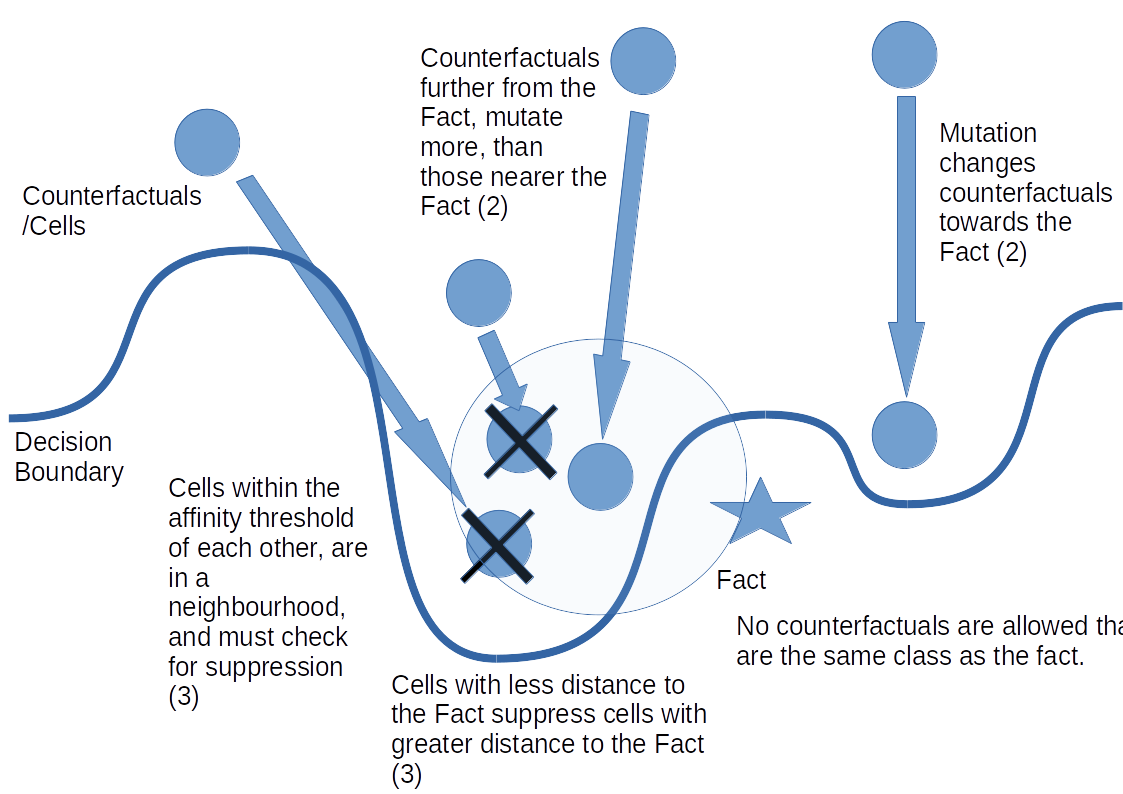
\includegraphics[width=0.75\textwidth]{images/aide.png}
    \caption{Image of how AIDE generates counterfactuals using the processes above \cite{forrest2021contrastive}.}
    \label{fig:aide}
\end{figure}

% Hyperparameters table:
\begin{table}[h]
\centering
\begin{tabular}{|p{0.25\linewidth}|p{0.65\linewidth}|}
\hline
\multicolumn{1}{|c|}{\textbf{Hyperparameter}} & \multicolumn{1}{c|}{\textbf{Description}} \\
\hline
Initial Population Size
& Number of random valid counterfactuals generated initially. Sometimes this needs to be overestimated since a cell is discarded if a new cell is not valid within a certain limit. \\
\hline
Number of New Cells
& Maximum new cells generated per generation\\
\hline
Number of Generations
& Maximum number of iterations unless stop condition is reached. \\
\hline
Stop Condition &  if the average cell cost falls below this value, the algorithm terminates. \\
\hline
Mutation Rate ($\beta$)
& Controls the magnitude of mutations; lower for fitter counterfactuals. \\
\hline
Affinity Constant
& This value is inversely proportional to the suppression threshold $\sigma$ is the most crucial parameter that establishes a neighborhood by defining a affinity around each counterfactual cell. When $\sigma$ is set to high values, it creates expansive suppression neighborhoods in which only the strongest counterfactuals live, ultimately yielding fewer but more diverse options. In contrast, lower $\sigma$ values result in smaller neighborhoods that allow a larger number of counterfactuals, albeit with less diversity. Consequently, it is essential to determine, for each individual model, dataset, and recipient, the optimal suppression threshold that generates the most effective set of counterfactuals for the user. \\
\hline
Invariants
&
Just like DiCE's actionably constraint, this is a list of features that cannot change. Hence, their value
can not be changed from the fact value in creating new random
cells or in the mutation process when cloned. \\
\hline
\end{tabular}
\caption{Table of the hyperparameters of the AIDE Algorithm \citep{forrest2021contrastive}.}
\label{tab:hyperparams}
\end{table}

\section{Benchmarking Counterfactual Explanations} \label{subsection:metrics}
%Ricardos work
A rigorous set of evaluation metrics is crucial for assessing both the quality of counterfactual explanations and the effectiveness of counterfactual explainer. The metrics proposed by \citet{guidotti2024counterfactual} and \citet{visani2022statistical}, are based on the characteristics detailed in \ref{subsection:properties}. In the subsequent discussion, the evaluation metrics are defined for an individual query instance $x$, where $C = f_k(x, b, X)$ represents the generated counterfactual set. The distance function is define as \(d(a, b) = \frac{1}{m_{con}} \sum_{i \in con} \frac{|a_i - b_i|}{MAD_i} + \frac{1}{m_{cat}} \sum_{i \in cat} \mathbb{1}_{a_i \neq b_i}\).

\begin{itemize}
    \item \textbf{Size}: Measures the proportion of counterfactuals generated relative to the maximum requested, emphasizing the ability to produce multiple explanations when applicable. $size =|C|/k$.
    
    \item \textbf{Dissimilarity}: Evaluates the proximity between the original instance and the counterfactuals, considering both feature-level sparsity and overall distance; lower values are better. \( dis_{\text{dist}} = \frac{1}{|C|} \sum_{x' \in C} d(x, x') \) and \( dis_{\text{count}} = \frac{1}{|C|\cdot m} \sum_{x' \in C} \sum_{i=1}^m \mathbb{1}_{x'_i \neq x_i} \).

    \item \textbf{Implausibility}: Assesses how realistic the counterfactuals are by measuring their distance from the nearest instances in the reference dataset, with smaller values indicating greater plausibility. \( impl = \frac{1}{|C|} \sum_{x' \in C} \min_{x \in X} d(x', x) \).

    \item \textbf{Discriminative Power}: Quantifies the effectiveness of counterfactuals in distinguishing between classes using a simple 1-Nearest Neighbor classifier; higher accuracy signifies better performance.
    
    \item \textbf{Actionability}: Measures the proportion of counterfactuals that can be practically implemented based on actionable features; higher values indicate better actionability $act = |\{x' \in C | A(x', x)\}|/k$, where the
    function a $A(x')$ returns $true$ if $x'$ is actionable w.r.t. the list of actionable features $A$, $false$ otherwise.
    
    \item \textbf{Diversity}: Evaluates the variety among counterfactuals in terms of both feature differences and overall distance, with greater diversity being preferable \( div_{dist} = \frac{1}{|C|^2} \sum_{x' \in C} \sum_{x'' \in C} d(x', x'') \quad div_{count} = \frac{1}{|C|^2 m} \sum_{x' \in C}\sum_{x'' \in C} \sum_{i=1}^{m} \mathbb{1}_{x'_i \neq x''_i} \).
    
    \item \textbf{Instability}: Captures the variation in counterfactuals generated for similar instances or under repeated runs, where lower instability reflects greater consistency \(inst_{x,\bar{x}} = \frac{1}{1 + d(x, \bar{x})} \frac{1}{|C||\bar{C}|} \sum_{x' \in C} \sum_{x'' \in \bar{C}} d(x', x'')\).
    
    \item \textbf{Runtime}: Measures the computational efficiency of generating counterfactuals, with shorter runtimes being more desirable.
\end{itemize}
\chapter{Problem Specification\label{chap:problem-spec}}
% Not more than 3 pages
% Fitness is the pushing action
In this study, an experiment is conducted to statistically compare DiCE and AIDE based that combines both quantitative and qualitative evaluations of counterfactual explanation methods. the metrics as defined in section \ref{subsection:metrics}. The genetic method that comes along in DiCE's package is also evaluated since it is mechanistically similar to AIDE and was not compared previously in \citet{guidotti2024counterfactual}. Additionally, a qualitative approach is taken by juxtaposing the counterfactuals onto the dataset using a parameter coordinate plot.

On the qualitative front, this visualization technique enables us to explore how changes in individual parameters are spread in the dataset, offering an intuitive visualization of the of counterfactual explanations. By mapping the counterfactuals onto the dataset, we can determine if the metrics agree with the data and the underlying mechanisms behind each method. we can identify clusters, outliers, and trends that might not be apparent through statistical metrics alone. The combination of statistical metrics and qualitative visualization provides a thorough assessment of each method’s strengths and limitations, contributing valuable insights into the practical application of counterfactual explanation techniques. Using those insights, the research questions in section \ref{research-questions} can be addressed. 
%[Should I add hypothesis here?]
%\begin{center}
%\begin{itemize}
%    \item \textbf{RQ1:} Is AIDE, an immune inspired algorithim, is well suited for the task of Counterfactual generation compared to DiCE? 
%    \item \textbf{RQ2:} Is AIDE well suited for the task of Counterfactual generation compared to GeCo?
%\end{itemize}
%\end{center}

\section{Selection of Explainer For the Experiment}
% Justify
So, why was DiCE chosen to go head to head with AIDE? According to categorization in \citet{guidotti2024counterfactual}, both explainers are quite similar. 
and DiCE was evaluated and performed as well as or better than all the counterfactual methods. This measure in performance provides a strong argument: if AIDE demonstrates superior results in our experiments, it would not only be considered better than DiCE but also compared to all of the other counterfatual explainers.

\begin{table}[ht]
\centering
\hspace*{-1.5cm} 
\begin{tabular}{|l|l|l|l|l|l|l|l|l|l|l|l|}
\hline
\textbf{Name} & \textbf{Strategy} & \textbf{\shortstack{Model\\Agno.}} & \textbf{\shortstack{Data\\Agno.}} & \textbf{Cat.} & \textbf{Validity} & \textbf{Action.} & \textbf{Causality} & \textbf{Exogen.} & \textbf{Multiple} \\ \hline
DiCE & OPT & DIF & TAB  & Yes  & Yes & Yes & No & Yes   & Yes    \\ \hline
GECO & HSS  & Yes  & TAB & Yes  & Yes   & Yes   &  No  & Yes   & Yes   \\ \hline
AIDE & OPT  & DIF  & TAB & Yes  & Yes   & Yes   & No  & Yes   & Yes   \\ \hline
\end{tabular}
\caption{Table that expands \citet{guidotti2024counterfactual}'s taxonomy by adding an entry for AIDE.}
\label{tab:taxonomy}
\end{table}

\section{The Datasets}
% Justify
In order to maintain consistency in the results, the datasets chosen were the same as in \citet{guidotti2024counterfactual}'s experiment. These datasets are tabular, which is common in XAI research, and widely recognized as standard benchmarks within the field. The datasets are:

\begin{itemize}
    \item \textbf{adult:} often called the Census Income dataset, is extracted from the 1994 US Census and is used to predict whether an individual earns over \$50K per year \citep{dua2017uci}.
    \item \textbf{fico:} The dataset consists of anonymized consumer credit records that include various financial attributes such as credit history, outstanding debt, and payment behavior. It is used for developing and evaluating credit scoring models as well as for research into fairness in lending \citep{chen2018interpretable}.
    \item \textbf{compas:} This dataset contains recidivism risk scores and related criminal history information for defendants from Broward County, Florida. It has been extensively analyzed in studies on algorithmic fairness and bias in criminal justice decision-making \citep{washington2018argue}.
    \item \textbf{german\_credit:} Also known as the German Credit Data, this dataset provides demographic and financial information about individuals to classify credit risk \citep{elsas1998relationship}. 
\end{itemize}

% Should I go into more detail here or next chapter?
\section{The Measured Metrics \label{sec:measured-metrics}}
% Justify

The chosen metrics for this experiment are Size, Dissimilarity, Runtime, Actionability, Diversity. This selection ensures an exhaustive evaluation while accounting for time constraints.

Metrics like Instability do not improve explanation quality nor does it matter to the end user. Although Implausibility does improve the quality of an explanation, Actionability has a higher influence to enforce realism. Lastly, Discriminative Power as mentioned in section \ref{subsection:properties} is most certainly better measured using human participants to visualize the changes in the counterfactual and query instance like done in \citet{forrest2021contrastive}. Therefore, the chosen metrics form a comprehensive set that prioritizes properties that are user centric, practical, and qualitative.

\section{The Data Perspective}
% Justify
A foundational aspect of any robust data analysis a deep understanding of the underlying data \citep{tukey1977exploratory}. This aligns perfectly with the principles of Exploratory Data Analysis (EDA), which emphasizes the necessity of scrutinizing data to uncover patterns, validate assumptions, and formulate hypotheses before formal modeling. The characteristics inherent to the dataset significantly shape the behaviour of machine learning models, thereby likely influencing the nature and reliability of the explanations they produce. Therefore, a diligent exploration of the data's distributions, inter-feature relationships, and potential inherent biases is vital.

The tipping case study offers a clear illustration of how exploratory and confirmatory approaches can complement one another in data analysis \citep{cook2025}. In this example, a restaurant’s tipping data is first transformed by calculating a tip percentage, an intuitive re-expression of the raw values. Initially, a full linear model is fitted using multiple predictors (such as total bill, party size, sex, smoker status, day, and time), yet the analysis reveals that only the size of the dining party significantly affects the tip percentage. By refining the model to include solely this predictor, the analysis underscores how a single variable can capture the essence of the tipping behavior, even though the refined model explains only a small fraction of the variance. This process, which involves creating insightful visualizations and diagnostic plots to assess model fit and underlying data patterns, embodies the spirit of EDA.

By prioritizing the visual exploration and thorough understanding of the data, researchers can enhance the robustness and interpretability of their findings, ultimately leading to more reliable evaluations of counterfactual and other XAI methods.

\chapter{Implementation\label{chap:implementation}}

%Issues and programming - 7 pages
%Steps i needed to take to run these algos
The project is available as a \href{https://github.com/Hariss-Gills/counterfactual_explainers}{Python package}. This will follow a similar approach to \citet{guidotti2024counterfactual}. A pain point throughout this project is the versioning of the \inlinecode{tensorflow} package. This is because DiCE and AIDE were developed with specific versions in mind. To combat this discrepancy, two different virtual environments (venv) are required. One with \inlinecode{tensorflow==2.13.0} for DiCE, and another with a newer \inlinecode{tensorflow==2.18.0} for AIDE. Moreover, there is a range  of a support Python versions for each \inlinecode{tensorflow} package. In this case, version \inlinecode{3.11.11} was chosen since it is the \href{https://www.tensorflow.org/install/source}{latest version} that is available for the two above versions.

\section{Encoding the Datasets}
Before the encoding step the compas dataset needed to be cleaned up. This is done by selecting key columns, converting date strings to datetime objects, and computing a new feature...\inlinecode{length\_of\_stay}. It normalizes the data by taking absolute values for fields that could have erroneous negative values and fills missing data with the most common values. 

A critical step in the data preprocessing pipeline is the encoding of categorical variables into numerical representations, enabling compatibility with the machine learning models. The configuration file (called \inlinecode{config.toml}) defines the encoding strategy for each dataset. For instance, in the adult, german\_credit, and compas datasets, categorical features are transformed using one-hot encoding. This approach creates binary indicator variables for each category, preserving the nominal relationships without imposing any artificial ordinal structure. In contrast, the fico dataset does not apply an encoding strategy, since all of its features are continuous. In addition, we define non-actionable features similarly to \citet{guidotti2024counterfactual} as the following:

\begin{itemize} \label{act-feat}
    \item \textbf{adult}: age, education, marital status, relationship, race, sex, native country.
    \item \textbf{compas}: age, sex, race.
    \item \textbf{fico}: external risk estimate.
    \item \textbf{german\_credit}: age, people under maintenance, credit history, purpose, sex, housing, foreign worker.

\end{itemize}

The encoding is integrated into our preprocessing pipeline via the \inlinecode{create\_data\_transformer} function, which dynamically selects the encoder based on the configuration. Once applied, the pipeline computes key statistics including the total number of features before and after encoding. This not only facilitates a quantitative evaluation of the dimensionality expansion caused by one-hot encoding but also helps to assess the impact on downstream model performance. The following are the properties of the dataset found by the \inlinecode{dataset\_stats.py} script avalible in the \inlinecode{dataset\_stats.csv} file in the results directory.


\begin{table}[ht]
\centering
\hspace*{-2.5cm} 
\resizebox{1.3\textwidth}{!}{%
\begin{tabular}{|l|r|r|r|r|r|r|r|}
\hline
\textbf{Dataset}         & \textbf{Num Recs} & \textbf{Num Feat} & \textbf{Num Cont Feat} & \textbf{Num Cat Feat} & \textbf{Num of Act Feat} & \textbf{Num of OHE Feat} & \textbf{Num of Labels} \\
\hline
adult           & 32561    & 12       & 4             & 8            & 5               & 12            & 2             \\
\hline
german\_credit  & 1000     & 20       & 7             & 13           & 13              & 20            & 2             \\
\hline
fico            & 10459    & 23       & 23            & 0            & 22              & NaN                & 2             \\
\hline
compas          & 7214     & 10       & 7             & 3            & 7               & 10            & 3             \\
\hline
\end{tabular}%
}
\caption{Table that provides feature information about the datasets. \textbf{Num Recs} denotes the total number of records in the dataset. \textbf{Num Feat} represents the total number of features. \textbf{Num Cont Feat} shows the count of continuous (numerical) features, while \textbf{Num Cat Feat} indicates the count of categorical (discrete) features. \textbf{Num of Act Feat} specifies the number of actionable features, and \textbf{Num of OHE Feat} displays the number of one-hot encoded features. Finally, \textbf{Num of Labels} refers to the number of label columns or target variables.}
\end{table}

\section{Training the Black Box Models}
The training of machine learning models for this project involves constructing, tuning, and evaluating two types of classifiers: a Random Forest (RF) and a Deep Neural Network (DNN). This can be found in \inlinecode{train\_models.py}. These models serve as the underlying black-box classifiers whose decisions are later explained using either as DiCE or AIDE. 
As previously explained, DiCE and AIDE utilize different versions of tensorflow, the training pipeline accommodates this by allowing the passing of arguments with \inlinecode{--explainer} or \inlinecode{-e} for shorthand. The implementation follows a structured workflow that encompasses model configuration, hyperparameter tuning, evaluation, and persistence.

\subsection{Model Configuration and Construction} The training process begins by reading the dataset configuration, defining the feature set, target variable, and associated encoding/scaling strategies. The \inlinecode{train\_and\_evaluate\_for\_dataset} function orchestrates the training and evaluation process. Key configuration elements include: 

\begin{itemize} \item \textbf{Random Forest:} The model is initialized with the \inlinecode{RandomForestClassifier()} class from \inlinecode{scikit-learn}. This model will be used for the GeCo algorithm in the \inlinecode{dice-ml} package.
\item \textbf{DNN:} Built dynamically using the \inlinecode{build\_dnn} function, which constructs a sequential neural network with configurable dimensions, activations, and dropout layers. By default, it uses a three-layer structure with ReLU activation and sigmoid activation for binary classification.
\end{itemize}

\subsection{Hyperparameter Tuning} To optimize the performance of the models, hyperparameter tuning is conducted using \inlinecode{RandomizedSearchCV}, which samples from a defined parameter space to identify the best-performing configuration. This search strategy balances computational efficiency with the exploration of potential parameter combinations. This can be improved by using a more exhaustive option like \inlinecode{GridSearchCV}. To facilitate this in \inlinecode{keras}, the \inlinecode{scikeras} package is used by providing a wrapper that has an \inlinecode{sklearn} interface. This did cause issue an though since \inlinecode{ClassifierMixin} does not have a superclass, the \inlinecode{Tags} class is used instantiate some tags. \citet{guidotti2024counterfactual}'s approach does not show how the DNN's were tuned.

The parameter space for Random Forest includes: 
\begin{itemize} 
\item \inlinecode{n\_estimators}: Number of decision trees in the ensemble.
\item \inlinecode{max\_depth}: Maximum depth of individual trees.
\item \inlinecode{min\_samples\_split}: Minimum number of samples required to split a node.
\item \inlinecode{min\_samples\_leaf}: Minimum number of samples required at a leaf node.
\item \inlinecode{class\_weight}: Balances class weights to address class imbalance
\end{itemize}

While the DNN has:
\begin{itemize}
    \item \inlinecode{dropout\_<layer>}: Dropout rates applied after the input and hidden layers.
    \item \inlinecode{dim\_1} and \inlinecode{dim\_2}: Dimensions of the first and second hidden layers.
    \item \inlinecode{activation\_<x>}: Activation functions for the input and hidden layers.
\end{itemize}

The \inlinecode{train\_model} function handles the construction of a machine learning pipeline that integrates the data preprocessing transformer and the classifier. Randomized search is then applied with 5-fold cross-validation to identify the best pipeline configuration. With a \inlinecode{random\_state} to ensure consistent results by setting the seed.

\subsection{Model Evaluation and Metrics} 
For each dataset, the data is split into training and testing sets using \inlinecode{train\_test\_split}, with stratification applied to preserve class distributions and a \inlinecode{test\_size=0.3}. Model performance is evaluated on both the training and test sets using multiple metrics to guarantee completeness. The below definitions are provided by \citet{burkov2020machine}.

\begin{itemize} 
\item \textbf{Accuracy:} Measures the number of correctly classified examples, divided by the total
number of classified example.
\item \textbf{F1 Macro:} Assesses the balance between precision and recall across all classes, weighted equally.
\item \textbf{F1 Micro:} Aggregates contributions from all classes to compute a single metric, providing insight into the overall predictive performance. 
\end{itemize}

The \inlinecode{evaluate\_model} function computes these metrics and stores the results for each trained model.
Thus, upon completing the training and evaluation, results are aggregated and saved to a CSV file named \inlinecode{training\_<explainer>.csv}, where \inlinecode{<explainer>} indicates the explainer framework used (either AIDE or DiCE). The results for the models used in the CF generation are provided below:


\begin{table}[htbp]
\centering
\hspace*{-2.5cm} 
\resizebox{1.3\textwidth}{!}{
\begin{tabular}{ll
                S[table-format=1.2]
                S[table-format=1.2]
                S[table-format=1.2]
                S[table-format=1.2]
                S[table-format=1.2]
                S[table-format=1.2]}
\toprule
{Dataset} & {Classifier} & {Accuracy Train} & {Accuracy Test} & {F1 Macro Train} & {F1 Macro Test} & {F1 Micro Train} & {F1 Micro Test} \\
\midrule
\multirow{2}{*}{adult}          
  & RF   & 0.87 & 0.86 & 0.80 & 0.79 & 0.87 & 0.86 \\
  & DNN  & 0.84 & 0.84 & 0.75 & 0.75 & 0.84 & 0.84 \\
\multirow{2}{*}{german\_credit}  
  & RF   & 0.82 & 0.75 & 0.80 & 0.72 & 0.82 & 0.75 \\
  & DNN  & 0.71 & 0.70 & 0.46 & 0.41 & 0.71 & 0.70 \\
\multirow{2}{*}{fico}           
  & RF   & 0.80 & 0.72 & 0.79 & 0.72 & 0.80 & 0.72 \\
  & DNN  & 0.70 & 0.69 & 0.69 & 0.68 & 0.70 & 0.69 \\
\multirow{2}{*}{compas}         
  & RF   & 0.69 & 0.59 & 0.65 & 0.55 & 0.69 & 0.59 \\
  & DNN  & 0.61 & 0.59 & 0.49 & 0.48 & 0.61 & 0.59 \\
\bottomrule
\end{tabular}}
\caption{Table displaying the performance metrics for DiCE's Black Box classifiers on the Datasets (Rounded to Two Decimal Places). They are slightly different to the results in \citet{guidotti2024counterfactual} due to the seeding.}
\end{table}

\begin{table}[htbp]
\centering
\hspace*{-2.5cm}
\resizebox{1.3\textwidth}{!}{
\begin{tabular}{ll
                S[table-format=1.2]
                S[table-format=1.2]
                S[table-format=1.2]
                S[table-format=1.2]
                S[table-format=1.2]
                S[table-format=1.2]}
\toprule
{Dataset} & {Accuracy Train} & {Accuracy Test} & {F1 Macro Train} & {F1 Macro Test} & {F1 Micro Train} & {F1 Micro Test} \\
\midrule
adult            & 0.81 & 0.81 & 0.65 & 0.64 & 0.81 & 0.81 \\
german\_credit   & 0.76 & 0.71 & 0.64 & 0.56 & 0.76 & 0.71 \\
fico             & 0.70 & 0.70 & 0.70 & 0.69 & 0.70 & 0.70 \\
compas           & 0.62 & 0.62 & 0.54 & 0.54 & 0.62 & 0.62 \\
\bottomrule
\end{tabular}}
\caption{Table displaying the performance metrics for AIDE's DNN Classifier on the Datasets (Rounded to Two Decimal Places).}
\end{table}

\subsection{Model Persistence}
To facilitate downstream counterfactual generation and reproducibility, the trained models are saved locally. The \inlinecode{save\_model} function handles this so that models are saved with descriptive filenames that include the model type, dataset name, and explainer framework used. While DNN models are saved in \inlinecode{.keras} format to preserve model architecture, weights, and configuration, the Random Forest models are serialized using \inlinecode{joblib} and stored in \inlinecode{.pkl} format.

\section{Generating Counterfactual with DiCE}
The generation of counterfactual explanations using the DiCE framework is done in \inlinecode{gen\_cfs\_dice.py}. It uses the models trained in the previous step with the actionability constraints in section \ref{act-feat} and the \inlinecode{dice-ml} package. This process is implemented in the \inlinecode{generate\_cfs\_for\_dataset} function, which implements the model loading, data transformation, and counterfactual generation. For some reason, \citet{guidotti2024counterfactual}'s approach does encodes the data before passing it over to DiCE even though the documentation recommends using the internal methods.

\subsection{DiCE Initialization}
DiCE requires three core objects for explanation generation:
\begin{itemize}
    \item \textbf{Data Object:} Encapsulates the training data and metadata (continuous/categorical features, target variable). Constructed from the training set using \inlinecode{Dice\_ml.Data()}. Since the sklearn models are wrapped in a pipeline object, the datasets target variables do not need to be explicitly encoded unlike models with a tensoflow backend. 
    \item \textbf{Model Object:} Wraps the Black Box model with a backend interface. For Random Forests (RF), the \inlinecode{sklearn} backend is used, while Deep Neural Networks (DNNs) employ the \inlinecode{TF2} backend with a \inlinecode{ohe-min-max} normalization function. This initially, caused a lot of issues since by default DiCE's implementation does not impute the dataset with \inlinecode{ohe-min-max}. So, the dimensions of the input data was larger than what the model accepts. To remedy this, DiCE does provide the option to pass in a transformation function to the \inlinecode{FunctionTransformer} object. However, you \href{https://github.com/interpretml/DiCE/blob/f93a2d35937f451d8340363895699859d862a6da/dice_ml/utils/helpers.py#L329}{cannot} pass in a \inlinecode{inverse\_func} to decode the data. This makes the generated CFs very hard to interpret to the end user which is not in the spirit of XAI. Consequently, this implementation simply imputes the dataset before handling the encoding to DiCE. Regardless, the \inlinecode{func} parameter is more suitable for the Model Object. 
    \item \textbf{Dice Object:} Points to different implementations of DiCE based on different frameworks such as Tensorflow or PyTorch or sklearn. So this implementation uses \inlinecode{"genetic"} method for RF models and \inlinecode{"gradient"} for DNN models.
\end{itemize}

\subsection{Counterfactual Generation Process}
For each dataset, a specific query instance is sampled, the process:
\begin{enumerate}
\item Configures actionable features by excluding non-actionable attributes defined in the dataset configuration. Yet again, this would be better tailored for the Data object. Also due, compas's ternery classification, a specific target class is given.
\item Generates counterfactuals iteratively for increasing required counts (1 to 20 CFs).
\item Handles DiCE-specific exceptions (e.g., \inlinecode{UserConfigValidationException}) when no valid CFs are found.
\item The counterfactuals and runtimes are saved to CSV files for further analysis.
\end{enumerate}

It is very important to note that the DiCE-compas and genetic-DiCE-fico combination failed to generate CFs for the specified query instance but did manage to find CFs for some other instances. This shows that DiCE cannot guarantee CFs for all query instances. 

\section{Generating Counterfactuals with AIDE}
The generation of counterfactual explanations using AIDE follows a fundamentally different paradigm compared to DiCE. Unlike DiCE, AIDE does not have a package so the code was reused from the \href{https://github.com/ColonelPride/AIDE_notebook/tree/master}{Jupyter Notebook} in \citet{forrest2021contrastive}. The script \inlinecode{aide\_explainer.py} demonstrates AIDE's unique approach to balancing exploration and exploitation in counterfactual search.

\subsection{Changes to AIDE}
In order to get AIDE running the following changes were added:

\begin{itemize}
    \item The code that writes to an sqlite DB was unnecessary so it was commented out.
    \item Using randomness, the initial population of counterfactual cells can be generated. Despite that, there is an upper limit constraint which was initially 10 and bumped up to a 100 to ensure the required initial population is reached, which often was not. This does unfortunetely increase runtime significantly.
    \item The trained models expected 2D tensors \inlinecode{(batch\_size=1, features)} while AIDE's predictions used 3D tensors. This was changed to handle the 2D inputs to return a prediction. Again due to compas's three classes, the two other classes compared to the query instance had to be merged.
    \item The dataframe returned from AIDE is not decoded. So the \inlinecode{decode\_df} function handles this to return the CFs in a human-readable form just like DiCE.
    \item In order to maintain consistency in encoding, the data reading functions were modified to use common \inlinecode{sklearn} strategies to get the data dictionary, which preserves categorical semantics.
\end{itemize}

\subsection{Dataset-Specific Hyperparameter Considerations}
%Another small improvement was to increase the new cell rate to 1.0. This is to not have a ridiculously high initial population size which would harm the runtime and improve any possible diversity lost.
The AIDE algorithm is not really designed to be run iteratively to return a specified number of counterfactuals. When taking an iterative approach similar to DiCE, the initial population was chosen to be around 50 to ensure that a large proportion of CFs are eliminated by the suppression process. Consequently, an optimal affinity constant (maximized to match the required amount but minimized to be as diverse as possible \ref{tab:hyperparams}) needs to be found for each specified number of counterfactuals. This is a very challenging task that requires an exhaustive search for every dataset and required number of CFs. 

During a few runs using the iterative approach, it was found that AIDE is very stable; i.e., if $x$ CFs were required the same $x-1$ were present in a previous run. So in fact a single-shot run to generate 20 with an optimal affinity constant, would have an improved runtime but have a theoretical possibility of a set of less diverse CFs, which was not found in practice. Henceforth, the single-shot method was preferred and the first $x$ were chosen out of the 20 CFs, where $x$ is the required number of CFs. The \inlinecode{DATASET\_PARAMS} dictionary contains these optimal values for the 20 required CFs.

\subsection{Counterfactual Generation Process}  
For each dataset and same query instance, AIDE employs a single-shot generation strategy:  
\begin{enumerate}  
    \item Initializes an artificial immune explainer with parameters depending on the dataset.  
    \item Generates the 20 counterfactuals.
    \item Just like in DiCE, the decoded counterfactuals and runtimes are saved to CSV files as long as the output dataframe is not empty.
\end{enumerate}

It is also interesting to see that AIDE managed to generate the counterfactuals for the query instance in every dataset whereas DiCE struggled.
\section{Plotting and Calculating the Metrics}
With everything prepared, the next step is to evaluate the counterfactual explanations produced by the different methods. This evaluation relies on a set of quantitative metrics computed by the \inlinecode{calculate\_metrics.py} script and subsequently visualized and analyzed by the \inlinecode{plot\_results.py} script. It handles any File I/O exceptions handling missing counterfactuals.

\subsection{Metrics Calculation}
The \inlinecode{calculate\_metrics.py} script is responsible for quantifying the quality of generated counterfactuals based on several established criteria. It operates by first loading pre-generated counterfactual instances for a specific dataset, model (DNN or RF), and explainer (AIDE or DiCE) stored in csv files. For each combination of dataset, model, and explainer specified
in the configuration, it performs the following key steps:

\begin{enumerate}
    \item \textbf{Data Encoding for Metrics:} Although it is possible to calculate the metrics on the decoded data, it tends to skew the metrics way higher than the results in \citet{guidotti2024counterfactual}. So this implementation re-uses the data transformation pipeline defined earlier \inlinecode{create\_data\_transformer} to encode both the query instance and its counterfactuals. This ensures consistency in feature representation for metric calculations, handling continuous and categorical features appropriately.
    \item \textbf{Median Absolute Deviation (MAD) Calculation:} To normalize distances for continuous features, the Median Absolute Deviation (MAD) is calculated for each continuous feature using the training portion of the dataset (\inlinecode{calc\_mad}). Using MAD provides a robust measure of dispersion, less sensitive to outliers than standard deviation. A value of 1.0 is used if MAD is zero to prevent division by zero.
    \item \textbf{Metrics Computation:} For a given query instance and its generated counterfactuals (up to the requested number), the script computes the metrics defined in section \ref{sec:measured-metrics}.
    \item \textbf{Results:} The calculated metrics for each number of requested counterfactuals (from 1 to 20) are aggregated and saved into a dedicated metrics csv file.
\end{enumerate}

\subsection{Visualization and Statistical Analysis}
The \inlinecode{plot\_results.py} script utilizes the metric CSV files to provide plots for EDA and statistical analysis of the different counterfactual explanation methods. The plots are colored to easily distinguish the dataset (grey), the query instance (magenta), and counterfactuals from AIDE (green), DiCE (blue), and DiCE-genetic/GeCo (red). Its main functionalities include:

\begin{itemize}
    \item \textbf{Metric Plots:} For each dataset, this function reads the metric csv files for available methods (AIDE with DNN, DiCE with DNN, DiCE with RF). It then generates line plots using \inlinecode{plotly}'s scatterplots with lines, showing how each metric changes as the number of requested counterfactuals increases (from 1 to 20). Each method is represented by a different colored line on the plot, allowing for direct visual comparison. Subplots are used to display all metrics in a single figure. These plots are saved as interactive HTML files.

    \item \textbf{Parallel Coordinates Plots:} To visualize the relationship between the original data, the query instance, and the generated counterfactuals in the high-dimensional feature space, a parallel coordinates plot is generated using \inlinecode{plotly}'s \inlinecode{Parcoords} class. The procedure preprocesses the data (imputation and encoding of categorical features), combines the original dataset samples, the query instance, and the counterfactuals from different methods into one dataframe. Each feature and the target variable is represented as a vertical axis. Data points are shown as lines crossing these axes. This allows for visual inspection of where the query instance lies relative to the data, and how the counterfactuals modify features to achieve the desired outcome class. Yet again, the plots are saved as interactive HTML files.
    \item \textbf{Statistical Analysis:} Alongside plotting, the script performs statistical tests to determine if the observed differences in metric scores between the methods are statistically significant. For each metric within a dataset, it performs
    An Analysis of Variance (ANOVA) test to check for any significant difference across the means of the different CF methods. If the ANOVA result is significant, a pairwise Tukey Honest Significant Difference (HSD) test is performed to identify which specific pairs of methods have significantly different mean scores for that metric. Dataframes and csv files have been heavily used in the project to document everything, so without a doubt the results of these tests are also saved to csv files. This analysis is also performed across all datasets for each metric in the main execution block to assess overall performance trends.
\end{itemize}
\chapter{Results and Evaluation\label{chap:evaluation}}
% Around 9-10 pages
% Do I need to add experimental Design stuff here?
\section{Quantitative Outlook with the Metrics}
As previously outlined, the plots are colored to easily distinguish the counterfactuals from AIDE (green), DiCE (blue), and DiCE-genetic/GeCo (red). These charts are best viewed in the browser as \inlinecode{plotly} provides them as interactive HTML files and they can be filtered by explainer method in the case of overlaps.


\begin{figure}[!htbp]
    \centering
    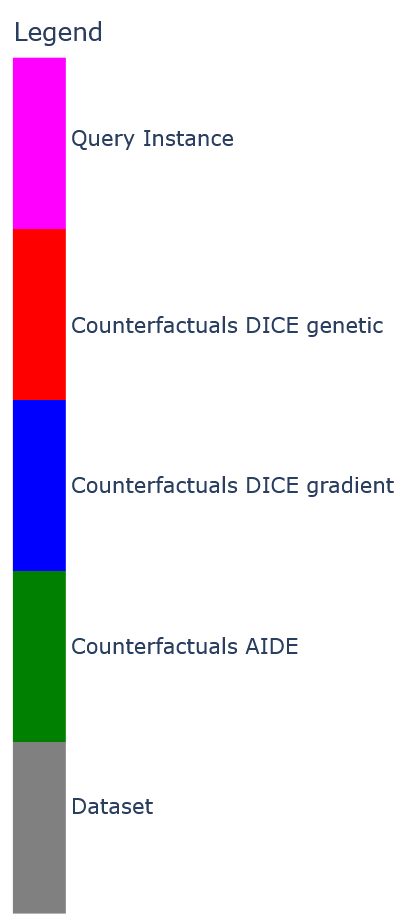
\includegraphics[angle=90, width=\textwidth]{images/legend.png}
    \caption{Image of the legend for the metric and parallel coordinates plots.}
    \label{fig:legend-plots}
\end{figure}
\begin{figure}[!htbp]
    \centering
    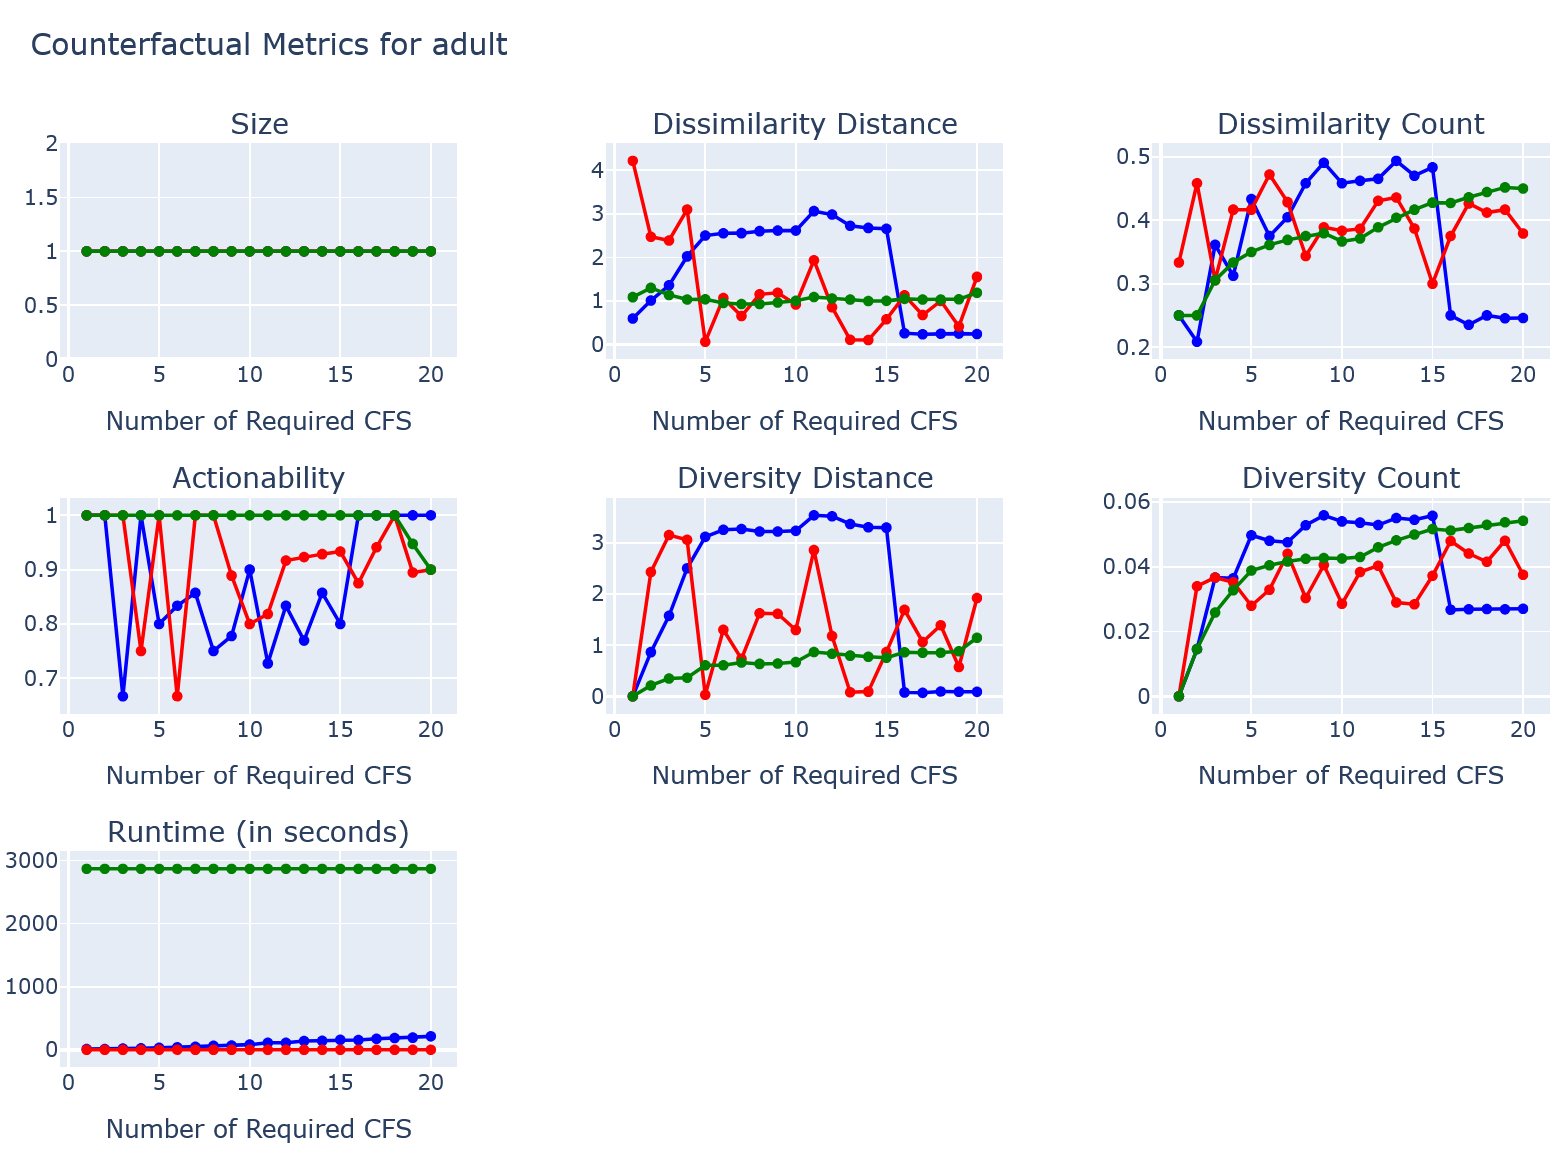
\includegraphics[width=\textwidth]{images/metrics-adult.png}
    \caption{Image of the metrics for the explainers on the adult dataset, varying the required number of
required counterfactuals.}
    \label{fig:metrics-adult}
\end{figure}
\begin{figure}[!htbp]
    \centering
    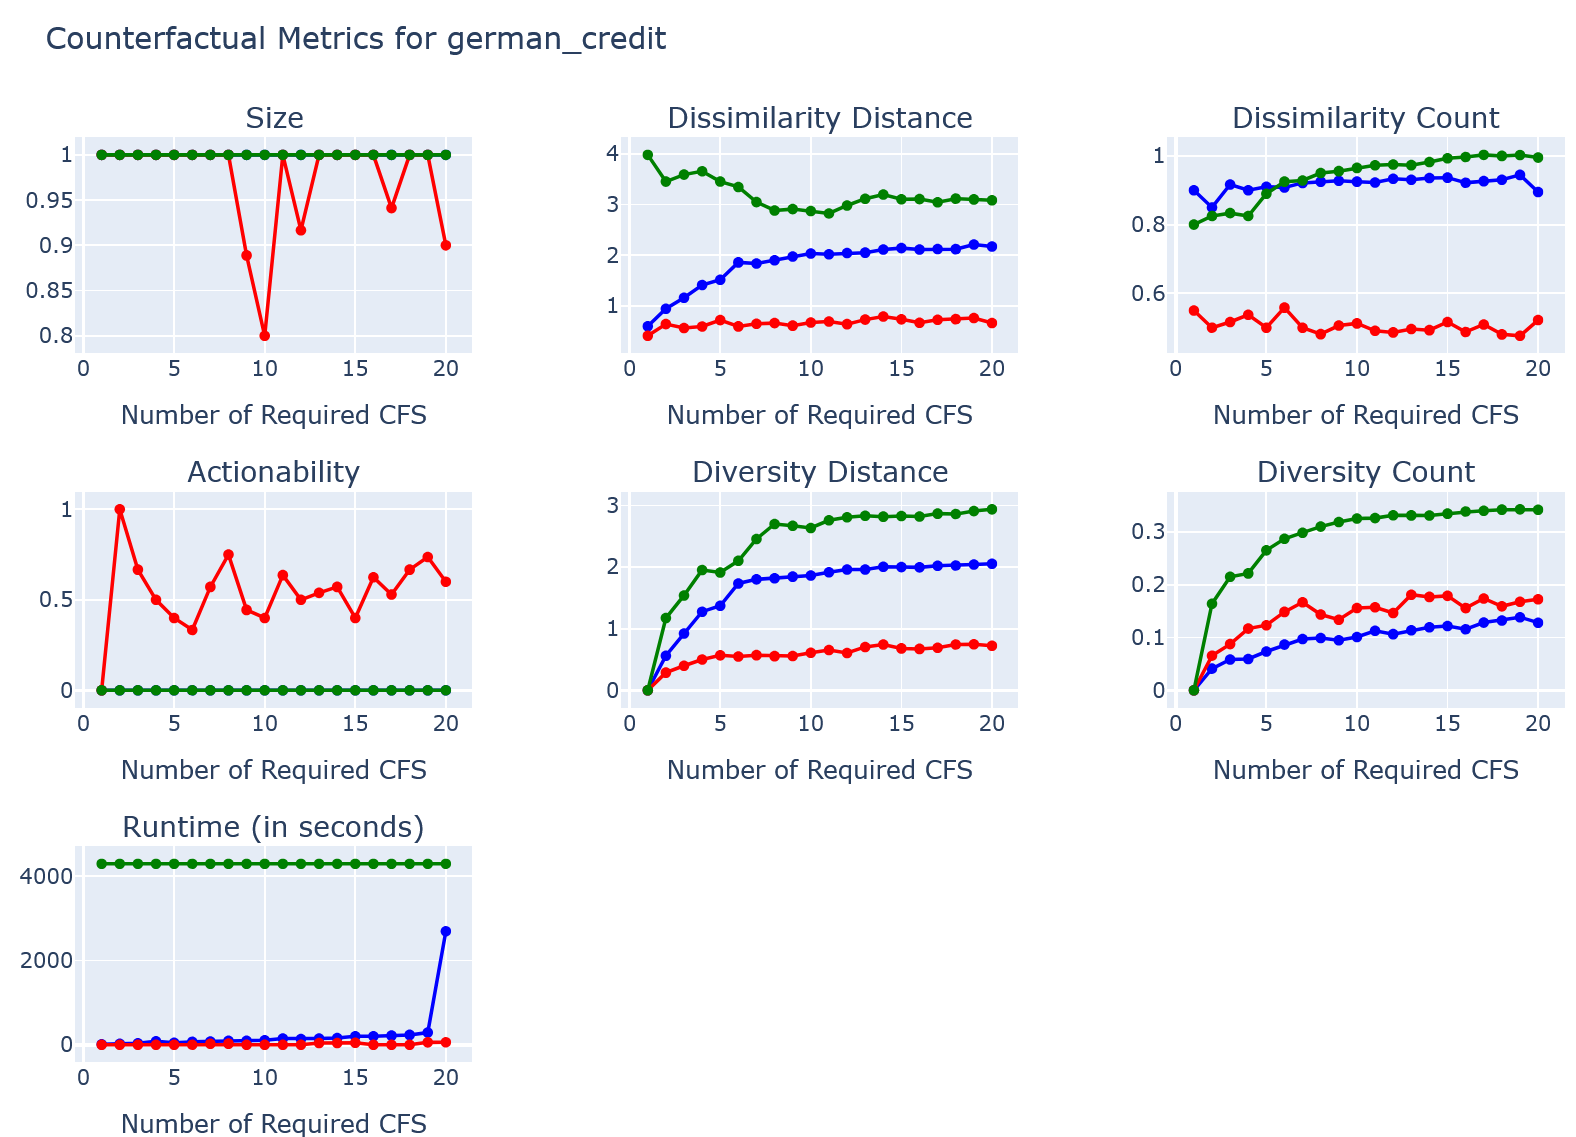
\includegraphics[width=\textwidth]{images/metrics-german_credit.png}
    \caption{Image of the metrics for the explainers on the german\_credit dataset, varying the required number of
required counterfactuals.}
    \label{fig:metrics-german_credit}
\end{figure}
\begin{figure}[!htbp]
    \centering
    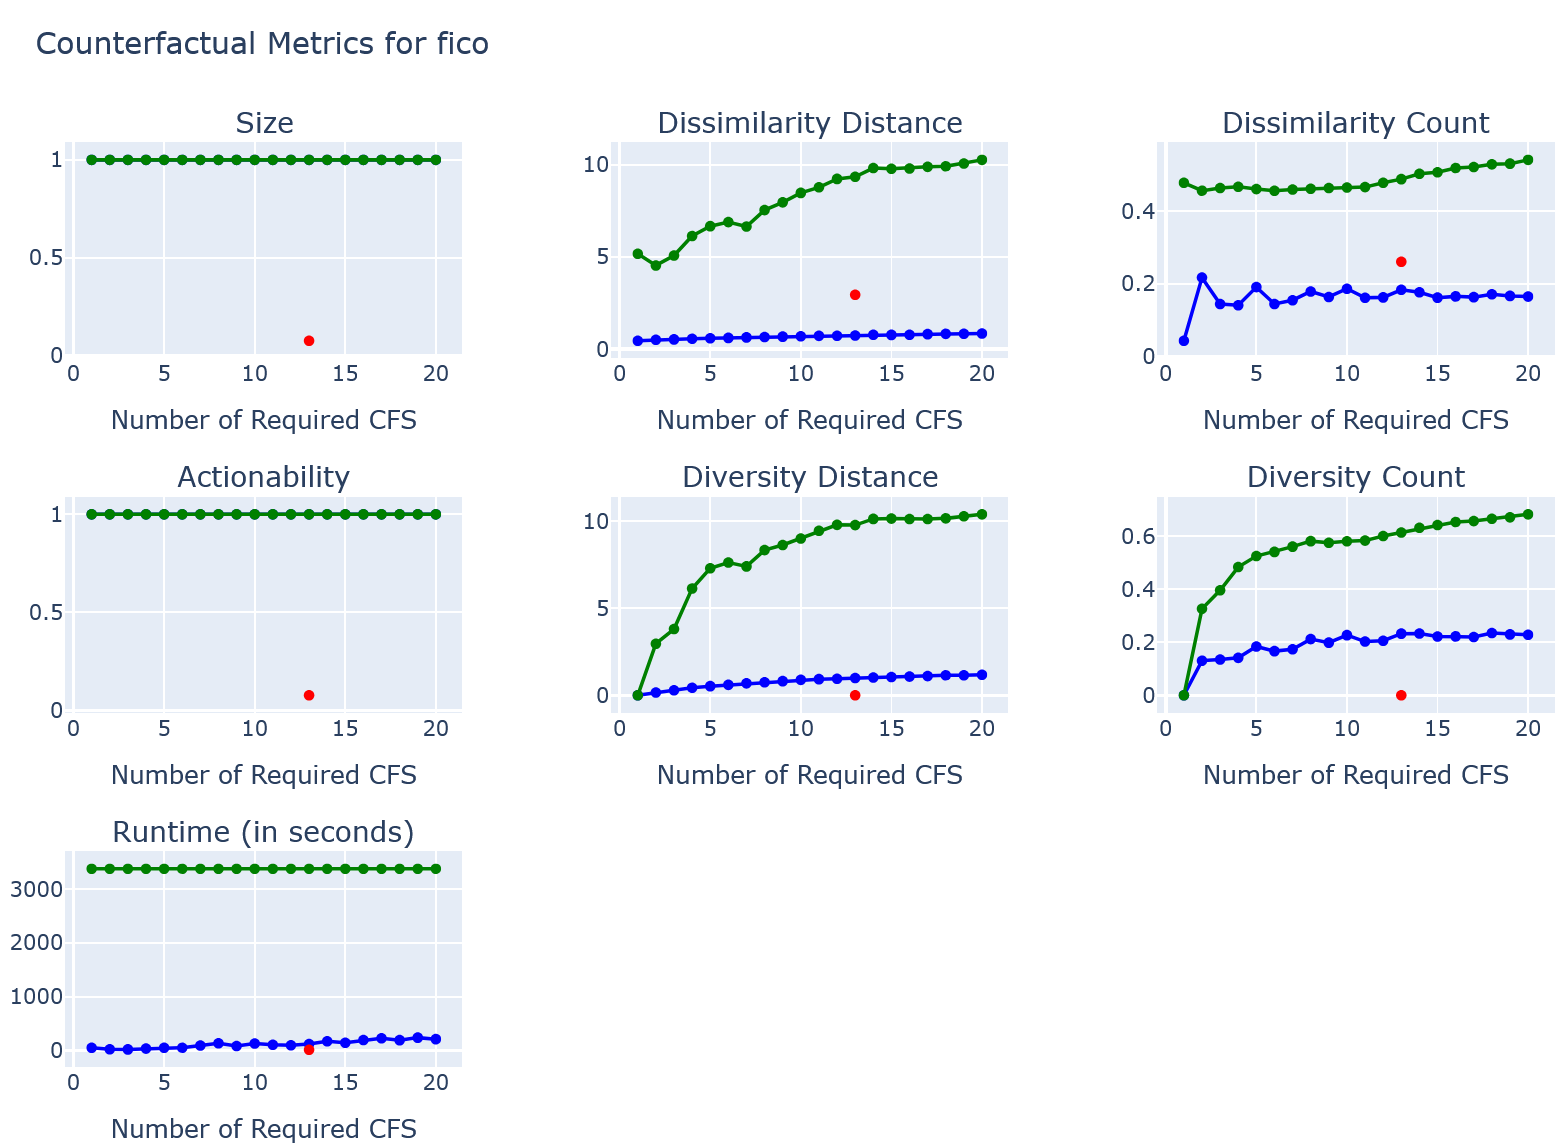
\includegraphics[width=\textwidth]{images/metrics-fico.png}
    \caption{Image of the metrics for the explainers on the fico dataset, varying the required number of
required counterfactuals.}
    \label{fig:metrics-fico}
\end{figure}
\begin{figure}[!htbp]
    \centering
    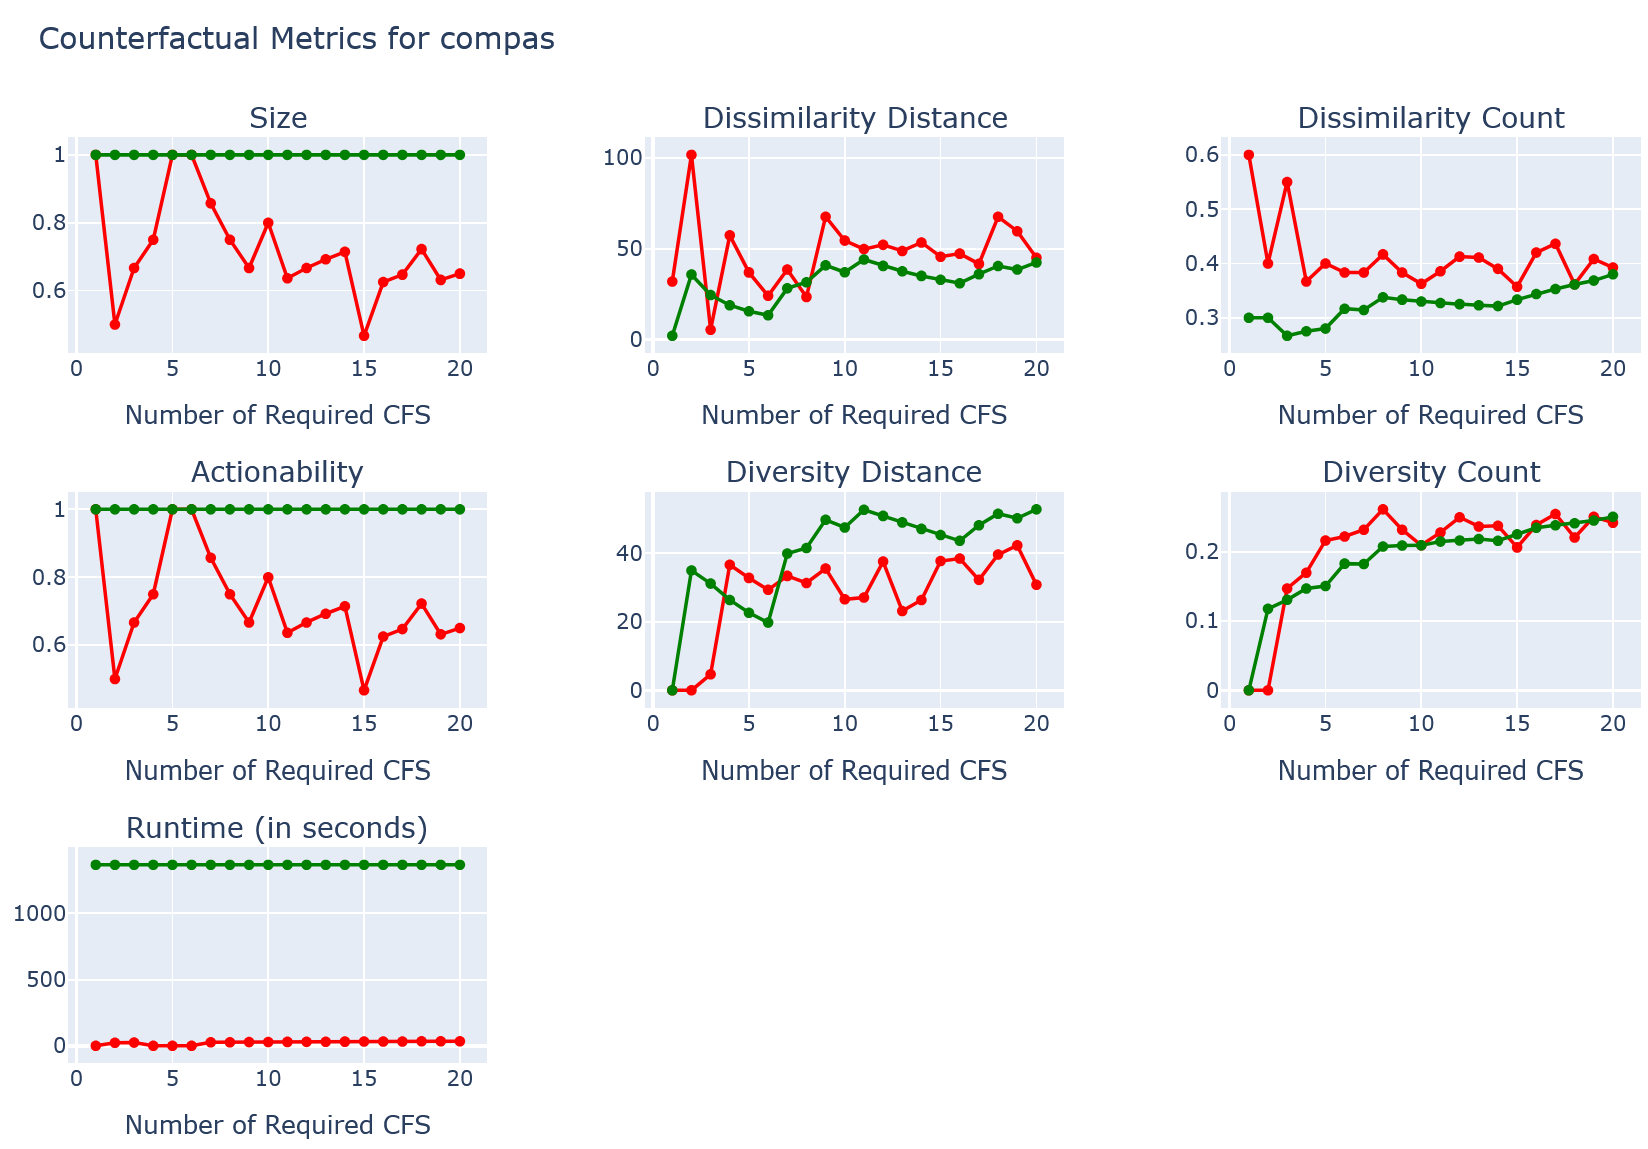
\includegraphics[width=\textwidth]{images/metrics-compas.png}
    \caption{Image of the metrics for the explainers on the compas dataset, varying the required number of
required counterfactuals.}
    \label{fig:metrics-compas}
\end{figure}

Let us examine each metric (left to right) to observe trends. For some certainty, it can be observed that the shape of the adult curves are similar to the ones in \citet{guidotti2024counterfactual} but more sharp. This makes sense, since the literature review averages the plots over all of the datasets. From the size plot, we notice that only DiCE-genetic fails to always return the required amount. Looking deeper into the algorithm this is clear since the genetic algorithm attempts to generate the specified number of CFs, but success depends on finding valid CFs that meet the desired outcome. If insufficient valid CFs are found within the iteration limit \inlinecode{maxiterations=5}, the result will contain fewer CFs. AIDE would likely have suffered from the same issue if the limit was not increased to 100. The constant size of 1 for AIDE is expected with the single-shot strategy and this is also a breeze for DiCE.

As for Dissimilarity, the count which accounts for feature level-sparsity does not seem to have large magnitudes of difference between the methods. However, it does seem that AIDE is worse, especially for when the number of required CFs is greater than 5. The Distances vary more greatly, other than fico it seems that AIDE is a lot more constant, DiCE-genetic jumps quite sharply, and DiCE rises constantly. DiCE also falls dramatically number of required CFs is greater than 15 for Adult. 

From the Actionability plot it can be observed that only AIDE return a large fraction of actionable CFs. There is some strange behavior in german\_credit where both DiCE and AIDE miserably fail. This is likely because of the amount of non-actionable columns and the long and complex column names after encoding. As \citet{guidotti2024counterfactual} points out this is expected since DiCE and it's genetic variant allow specifying the actionable features, but this check is not enforced for Validity or Actionability. On the other hand, AIDE attempts to mutate values in the set of actionable features. This is especially strange for the genetic variant since it was expected that GeCo's PLAF constraints to work it's magic, but it could that the package does not use the constraints. 

Diversity also seems to have a clear winner for counts and distance, which is AIDE. Interestingly, even though DiCE-genetic has a higher Dissimilarity distance than AIDE, AIDE has higher Diversity distance across all datasets. This shows that AIDE attempts to balance the trade-off in Diversity and Similarity. Yet again, DiCE's Diversity falls dramatically number of required CFs is greater than 15 for Adult, which is expected since of the known trade-off between Diversity and Similarity. 

Lastly, for Runtime it can be clearly seen that the $\Delta$-representation and partial evaluation in DiCE-genetic are optimizing the runtimes well. DiCE takes slightly longer to run but AIDE does take a much longer time to run. This is due to the increase in iteration limit by 10 times and due to the single-shot approach taken to generate the counterfactuals. 

\subsection{Statistical Tests}
After looking at the plots, let us employ statistical evaluation of the metrics. Since advantageous properties could be high (Diversity) or low (Dissimilarity), a One-way ANOVA (ANalysis Of VAriance) with post-hoc Tukey HSD (Honestly Significant Difference) is computed for each metric across all of the datasets. This was also computed per dataset and is available in the repository. This is done since we have three groups.
%[Should I add other precond].

\begin{table}[!htbp]
    \centering
    \centering
    \begin{tabular}{l l r r r r l}
        \toprule
        Group 1 & Group 2 & Mean Diff & p-adj & Lower & Upper & Reject \\
        \midrule
        AIDE & DiCE-genetic   & -0.1153 & 0.0 & -0.1564 & -0.0742 & True \\
        AIDE & DiCE  &  0.0000 & 1.0 & -0.0413 &  0.0413 & False \\
        DiCE-genetic & DiCE  &  0.1153 & 0.0 &  0.0713 &  0.1593 & True \\
        \bottomrule
    \end{tabular}
    \caption{Table of Tukey's HSD Test results for Size (ANOVA p-value = \SI{4.492443e-11}{})}
    \label{tab:tukey-results-size}
\end{table}

\begin{table}[!htbp]
    \centering
    \begin{tabular}{llrrrrl}
        \toprule
        Group 1 & Group 2 & Mean Diff & p-adj & Lower & Upper & Reject \\
        \midrule
        AIDE          & DiCE-genetic   &  5.3934  & 0.1207 &  -1.05   & 11.8369  & False \\
        AIDE          & DiCE  & -9.5077  & 0.0019 & -15.9815 &  -3.0338 & True  \\
        DiCE-genetic & DiCE  & -14.9011 & 0.0    & -21.7936 &  -8.0087 & True  \\
        \bottomrule
    \end{tabular}
    \caption{Table of Tukey's HSD Test results for Dissimilarity Distance (ANOVA p-value = \SI{3e-6}{})}
    \label{tab:tukey-results-dis-dist}
\end{table}

\begin{table}[!htbp]
    \centering
    \begin{tabular}{llrrrrl}
        \toprule
        Group 1 & Group 2 & Mean Diff & p-adj & Lower & Upper & Reject \\
        \midrule
        AIDE          & DiCE-genetic   & -0.0976 & 0.0479 & -0.1944 & -0.0007 & True  \\
        AIDE          & DiCE  & -0.0492 & 0.4582 & -0.1465 &  0.0481 & False \\
        DiCE-genetic & DiCE  &  0.0484 & 0.5139 & -0.0553 &  0.1520 & False \\
        \bottomrule
    \end{tabular}
    \caption{Table of Tukey's HSD Test results for Dissimilarity Count (ANOVA p-value = \SI{6.0451e-2}{})}
    \label{tab:tukey-results-dis-count}
\end{table}
\begin{table}[!htbp]
    \centering
    \begin{tabular}{llrrrrl}
        \toprule
        Group 1 & Group 2 & Mean Diff & p-adj & Lower & Upper & Reject \\
        \midrule
        AIDE          & DiCE-genetic   & -0.0329 & 0.8734 & -0.1897 & 0.1238 & False \\
        AIDE          & DiCE  & -0.1219 & 0.1633 & -0.2794 & 0.0356 & False \\
        DiCE-genetic & DiCE  & -0.0890 & 0.4235 & -0.2567 & 0.0787 & False \\
        \bottomrule
    \end{tabular}
    \caption{Table of Tukey's HSD Test results for Actionability (ANOVA p-value = \SI{0.181364}{})}
    \label{tab:tukey-results-act}
\end{table}

\begin{table}[!htbp]
    \centering
    \begin{tabular}{llrrrrl}
        \toprule
        Group 1 & Group 2 & Mean Diff & p-adj & Lower & Upper & Reject \\
        \midrule
        AIDE          & DiCE-genetic   &  -2.9441 & 0.4211 &  -8.4737 &   2.5856 & False \\
        AIDE          & DiCE  & -11.3308 & 0.0    & -16.8865 &  -5.7751 & True  \\
        DiCE-genetic & DiCE  &  -8.3867 & 0.0028 & -14.3016 &  -2.4718 & True  \\
        \bottomrule
    \end{tabular}
    \caption{Table of Tukey's HSD Test results Diversity Distance (ANOVA p-value = \SI{1.2e-5}{})}
    \label{tab:tukey-results-div-dist}
\end{table}

\begin{table}[!htbp]
    \centering
    \begin{tabular}{llrrrrl}
        \toprule
        Group 1 & Group 2 & Mean Diff & p-adj & Lower & Upper & Reject \\
        \midrule
        AIDE          & DiCE-genetic   & -0.1434 & 0.0    & -0.2017 & -0.0851 & True  \\
        AIDE          & DiCE  & -0.1587 & 0.0    & -0.2173 & -0.1001 & True  \\
        DiCE-genetic & DiCE  & -0.0153 & 0.8322 & -0.0776 &  0.0471 & False \\
        \bottomrule
    \end{tabular}
    \caption{Table of Tukey's HSD Test results for Diversity Count (ANOVA p-value = \SI{8.018792e-11}{})}
    \label{tab:tukey_results}
\end{table}
\begin{table}[!htbp]
    \centering
    \begin{tabular}{llrrrrl}
        \toprule
        Group 1 & Group 2 & Mean Diff & p-adj & Lower & Upper & Reject \\
        \midrule
        AIDE          & DiCE-genetic   & -2963.6502 & 0.0   & -3244.5292 & -2682.7712 & True \\
        AIDE          & DiCE  & -2819.7193 & 0.0   & -3101.9232 & -2537.5154 & True \\
        DiCE-genetic & DiCE  &   143.9309 & 0.496 &  -156.5187 &   444.3806 & False \\
        \bottomrule
    \end{tabular}
    \caption{Table of Tukey's HSD Test results for Runtime (ANOVA p-value = \SI{2.700452e-71}{})}
    \label{tab:tukey_results}
\end{table}


So to put it into text here is what was found:
\begin{itemize}
    \item \textbf{Size:} This is a tie between AIDE and DiCE. Both achieve perfect scores (1.0), while DICE-genetic is significantly worse. 
    \item \textbf{Dissimilarity Distance:} DiCE is the best performer with the lowest mean (1.43, AIDE: 10.94, DiCE-genetic: 16.33) with significant differences from others.
    \item \textbf{Dissimilarity Count:} DiCE-genetic only marginally significantly overcomes the other explainers (ANOVA p=0.06).
    \item \textbf{Actionability:} Although not statistically significant (ANOVA p=0.18), AIDE is the best here. if not for the unexpected behavior in german\_credit it would most likely been significant.
    \item \textbf{Diversity Distance:} AIDE is the most diverse (12.84, DiCE:1.54, DICE-genetic: 9.90). However, it does not significantly triumph over DiCE-genetic.
    \item \textbf{Diversity Count:} AIDE significantly prevails over both. But there is not a significant difference between the other explainers.
    \item \textbf{Runtime:} Despite DICE-genetic being faster than AIDE, it is not significantly faster than DiCE (Tukey HSD p=0.496).
\end{itemize}

Consequently for both of the research questions (\textbf{RQ1} and \textbf{RQ2}), even though AIDE performed well for the four out of the seven metrics it is not hands down better for generating counterfactuals than DiCE or genetic-DiCE. In order to dig deeper, the parallel coordinate plots will need to be looked at.

% Two parts to digging deep 
%Make conclusions about research question and open up new ones and go into Parallel Coordinate Plots. 
\section{Qualitative Outlook with the Parallel Coordinates Plots}
In the parallel coordinates plots, the dataset (gray), the query instance (magenta) are added. These counterfactuals are plotted for when the required number is 20. It is stressed that the charts are particularly better experienced on the browser. These plots are richly interactive. The lines can be dragged along the axes to filter regions and the axis can be dragged names across the plot to rearrange variables. This is useful for the target class. Another suggestion, is to view the german\_credit and fico plots on a wider display since the columns names are long and can be hard to distinguish in the plots.

\begin{figure}[!htbp]
    \centering
    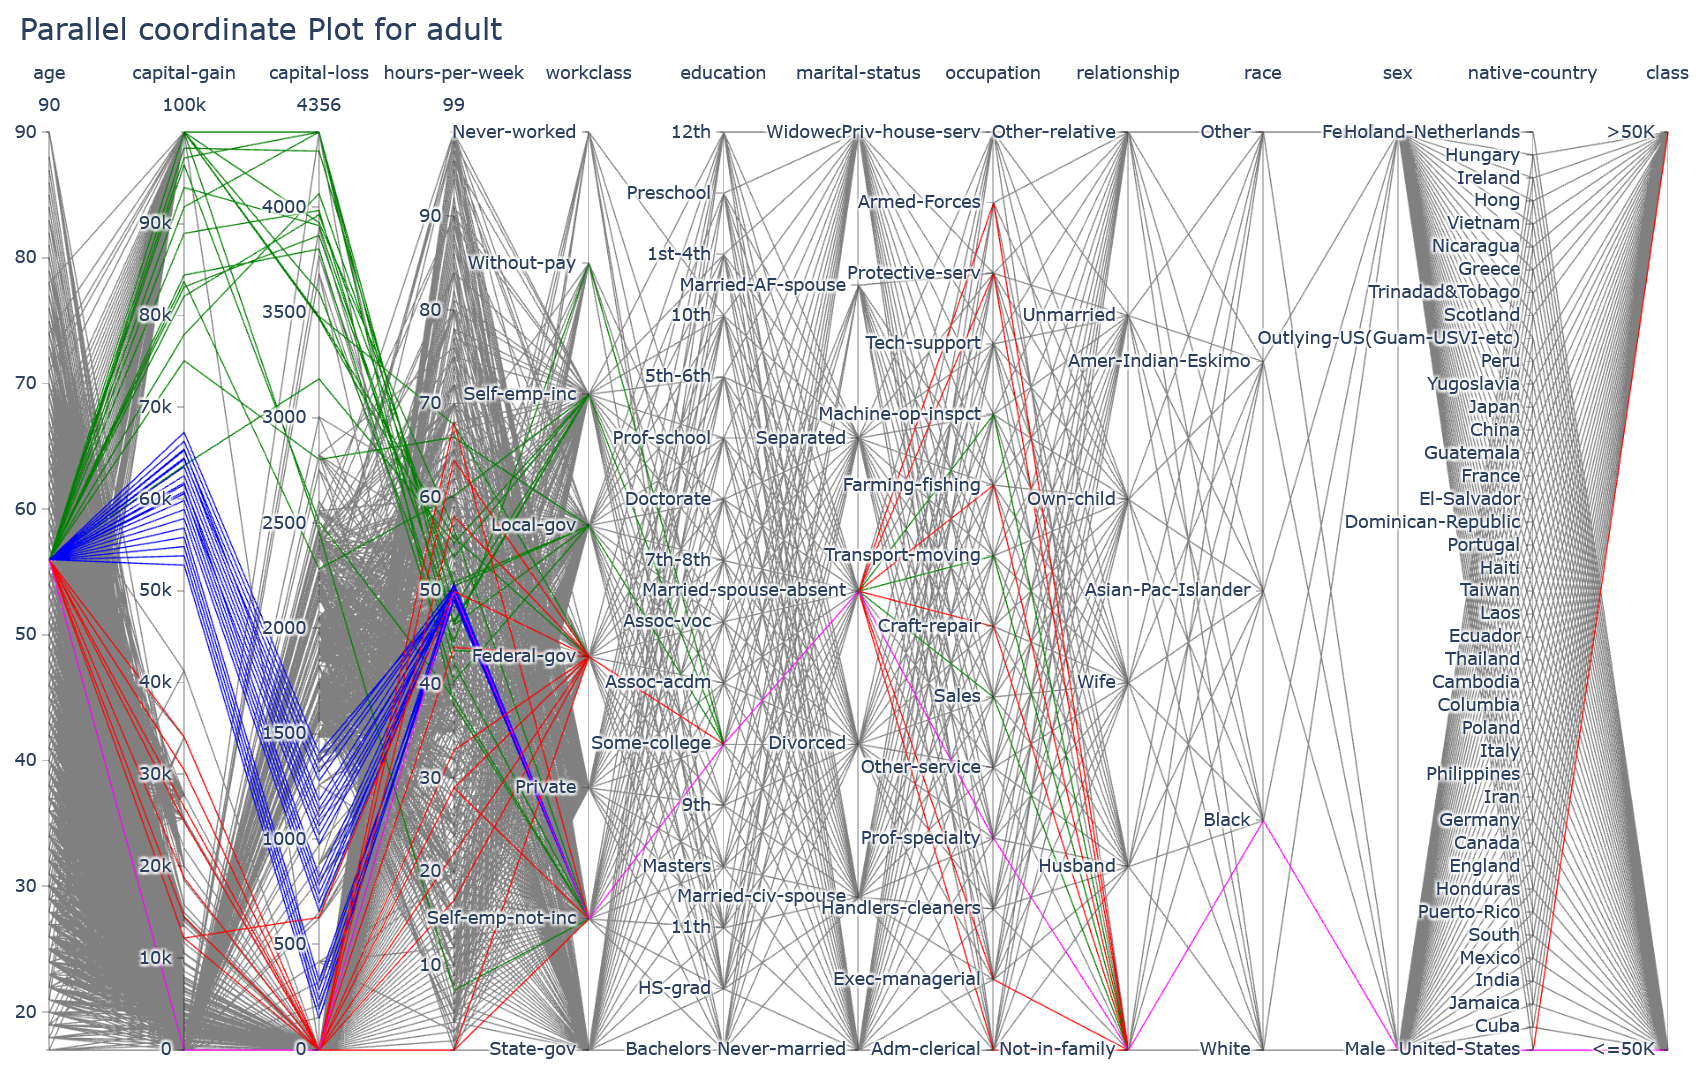
\includegraphics[width=\textwidth]{images/pcp-adult.png}
    \caption{Parallel coordinate plot for the explainers on the adult dataset.}
    \label{fig:pcp-adult}
\end{figure}

Due to space constraints, only the adult dataset will be analyzed thoroughly axis-by-axis. The actionability is pretty high across all explainers so the non-actionable columns (age, education, marital status, relationship, race, sex, native country) will be ignored. These will appear as if they are merging into the original query instance in the plot. For capital-gain, it can be seen that DiCE's CFs are in a range that the dataset is not and the deltas between each CFs are very similar. This is likely due to the "repulsions" from the \verb|dpp_diversity| term. On the other hand, AIDE and DiCE-genetic are on opposite sides of this spectrum. With AIDE selecting the higher-end while, DiCE-genetic opting for options closer to the query instance. 

A similar story can be seen with capital-loss, DiCE's CFs are again in a range of low concentration compared to the rest of the dataset. DiCE-genetic hurts itself here in terms of diversity since the capital-loss here is the same for all CFs (0). Likewise, AIDE's CFs are near the upper end of capital-loss.

hours-per-week experiences a different behavior compared to the above two axes. It's hard to gauge the deltas of DiCE but the values seems to concentrated around the query instances values (50). DiCE-genetic's values seem to jump around a lot here. This is likely why the  Dissimilarity is high. AIDE's values also jump around quite a bit but has clusters closer to the query instance due immune-network approach that tries to maintain multiple local optima.

For our first categorical feature, workclass, DiCE really struggles here not changing this variable for any counterfactual. DiCE-genetic does not perform much better only suggesting one other category... Federal-gov. These methods do this even though if the target is filtered there are a significant number of instances across six of the categories. AIDE does shine here but one CF does oddly suggest Without-pay where no other data point has a salary greater than 50k with that category.

Lastly, the other categorical feature, occupation, DiCE experiences the same issues. However, DiCE-genetic does significantly improve here maintaining many categories. AIDE still performs well here.

\begin{figure}[!htbp]
    \centering
    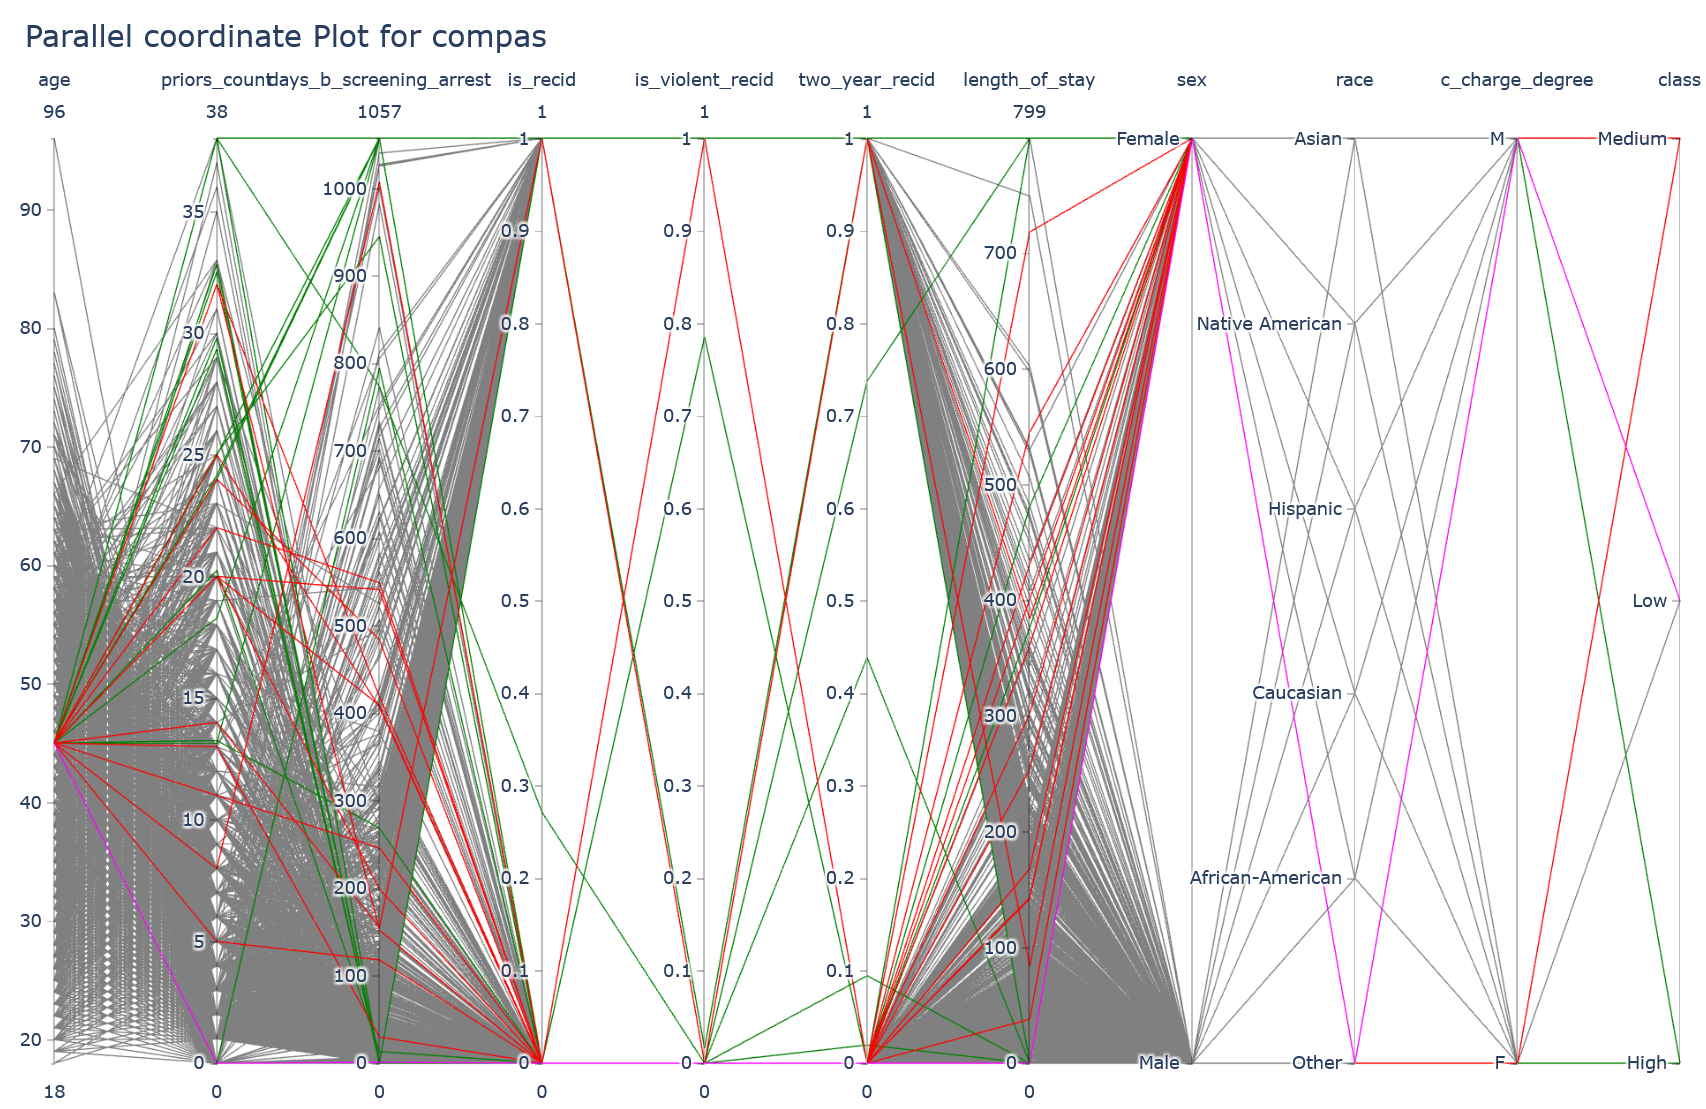
\includegraphics[width=\textwidth]{images/pcp-compas.png}
    \caption{Image of parallel coordinates plot for the explainers on the compas dataset.}
    \label{fig:pcp-compas}
\end{figure}
\begin{figure}[!htbp]
    \centering
    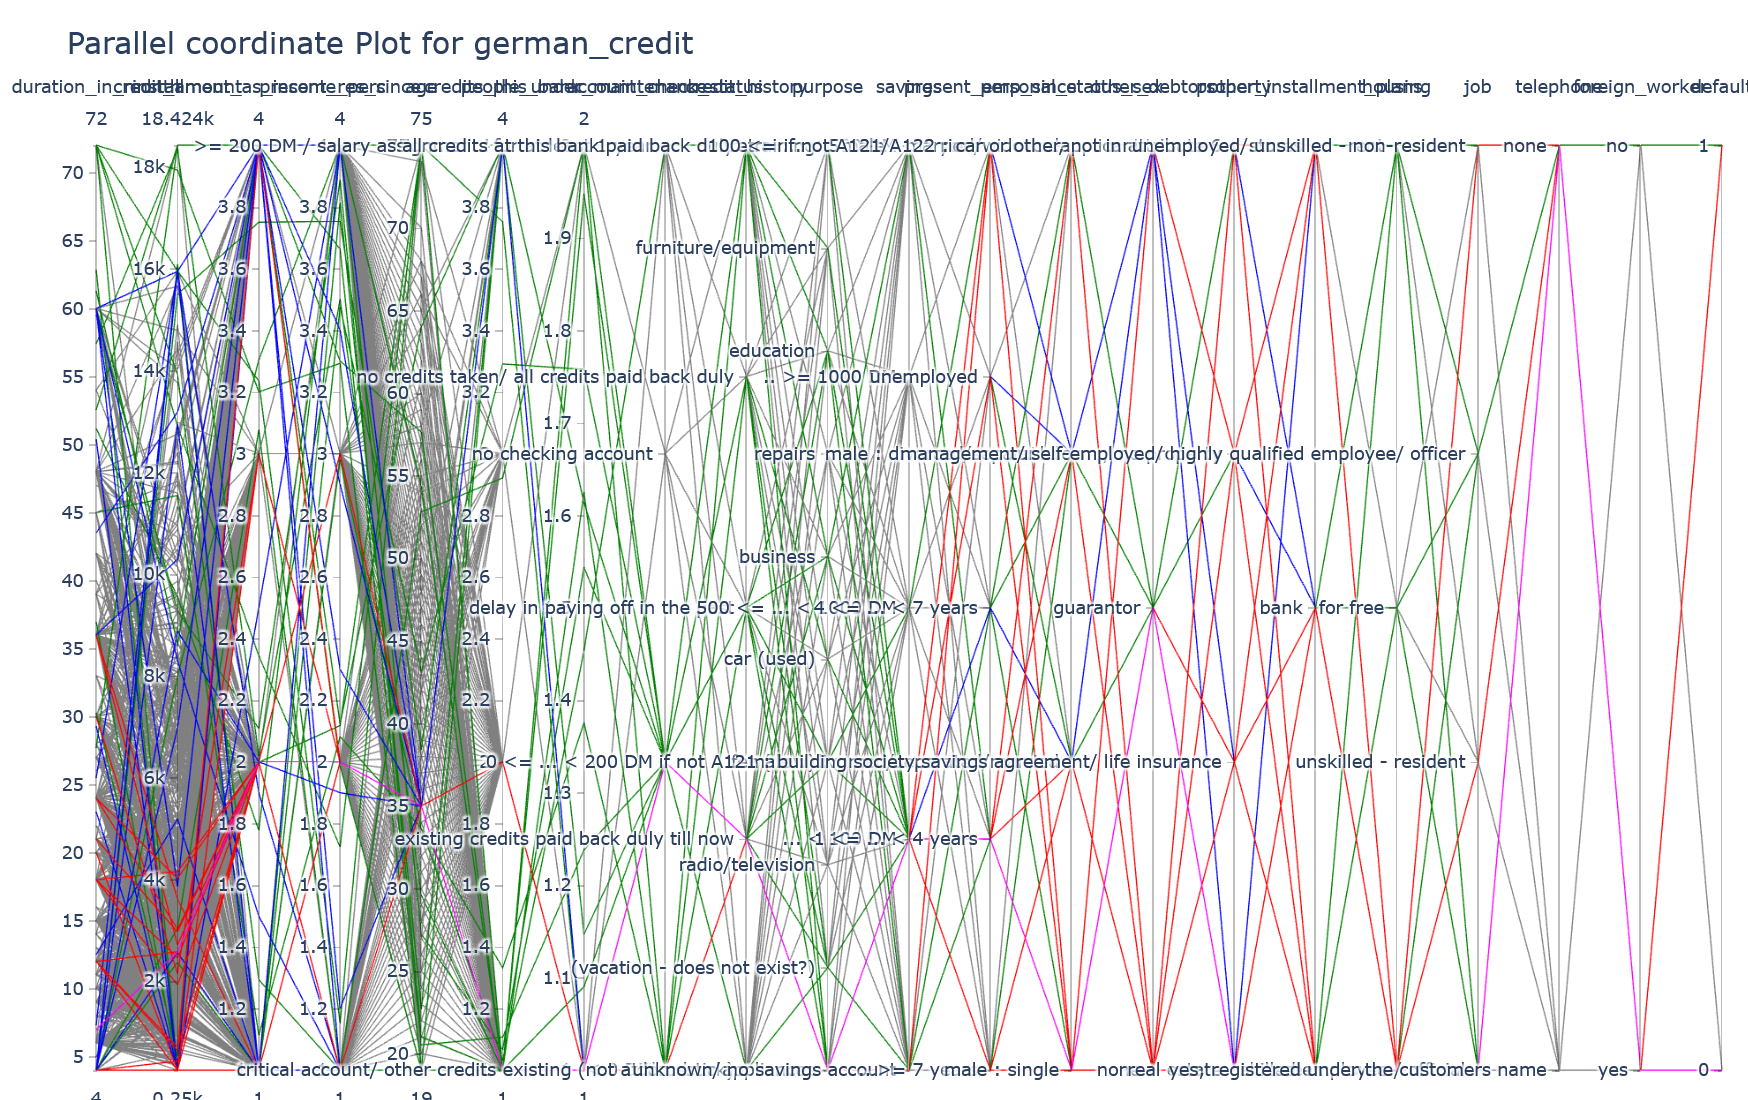
\includegraphics[width=\textwidth]{images/pcp-german_credit.png}
    \caption{Image of the parallel coordinates plot for the explainers on the german\_credit dataset.}
    \label{fig:pcp-german_credit}
\end{figure}
\begin{figure}[!htbp]
    \centering
    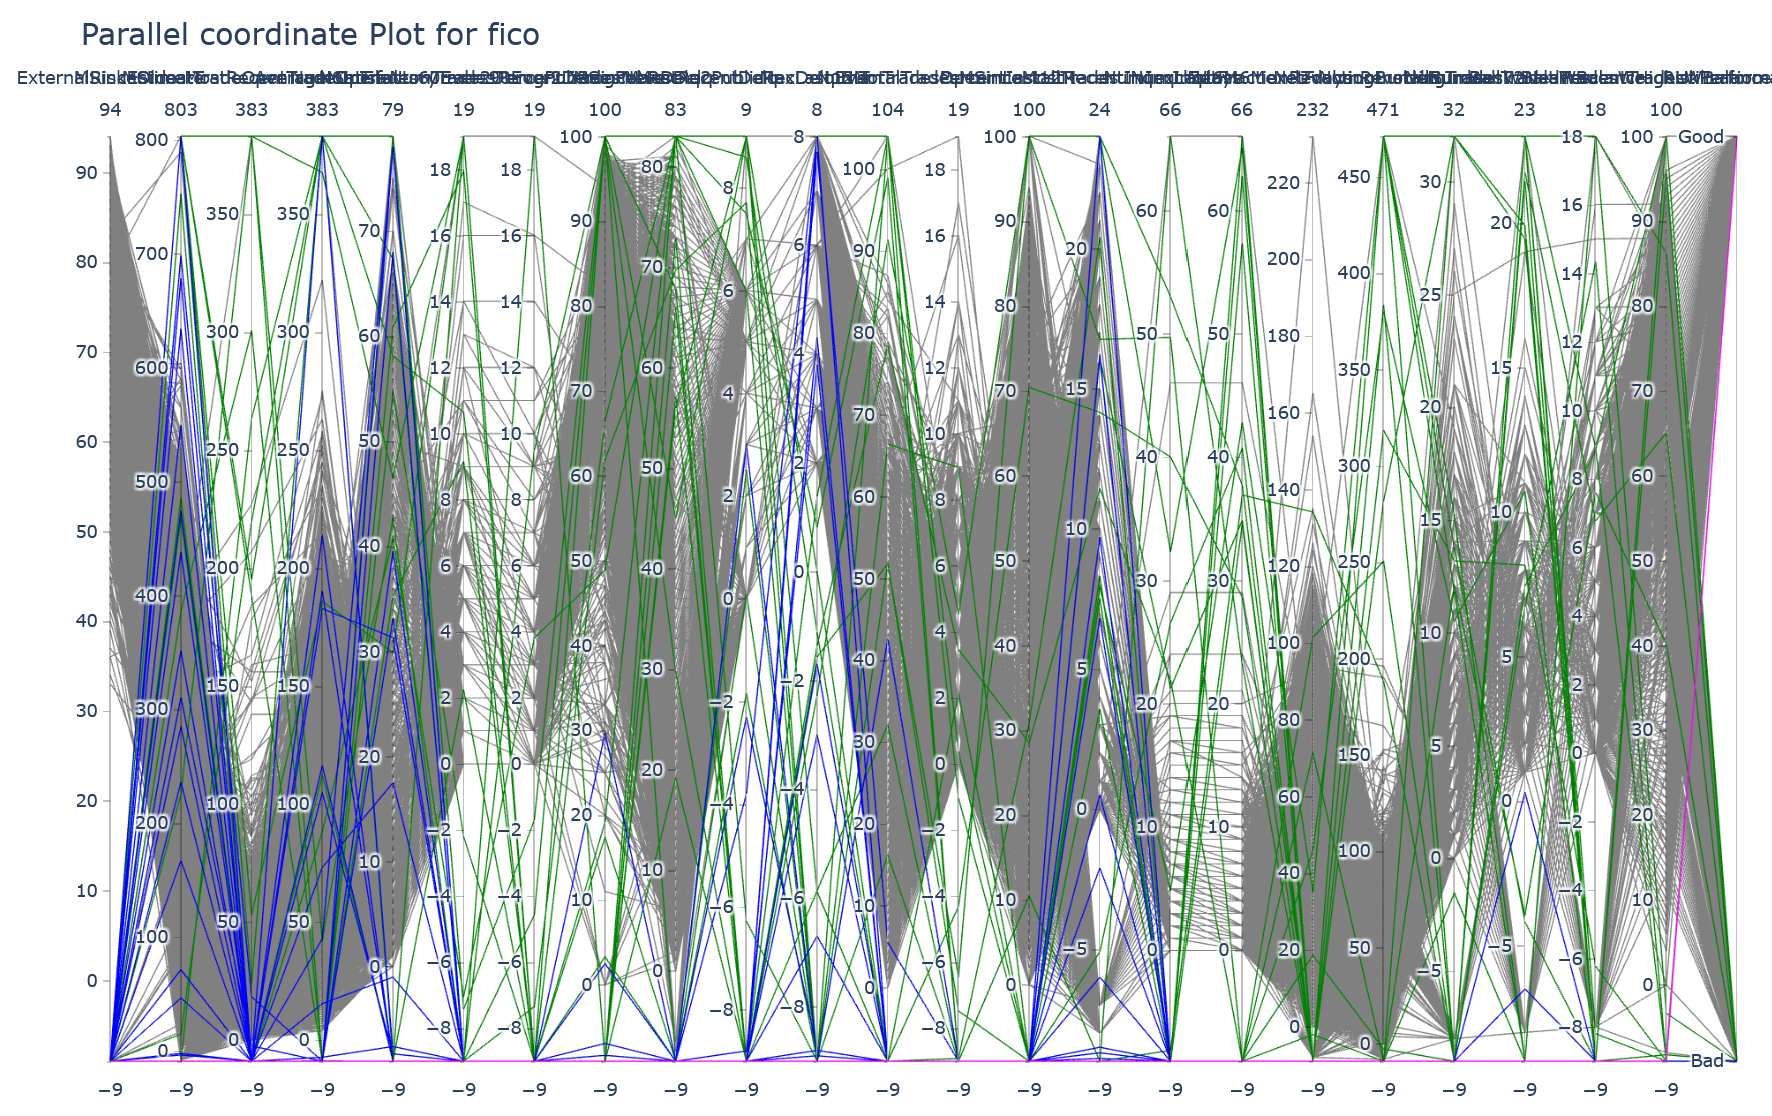
\includegraphics[width=\textwidth]{images/pcp-fico.png}
    \caption{Image of the parallel coordinates plot for the explainers on the fico dataset.}
    \label{fig:pcp-fico}
\end{figure}

What the above really suggests is that the counterfactual methods perform quite differently with between continuous and categorical features and that each method provides different kinds of counterfactuals. Given more time, the metrics could have also be measured separately for continuous and categorical features to find differences. Additionally, the metrics defined in section \ref{subsection:metrics} can be expanded since the Implausibility metric only measures the distances with respect to the nearest instance in the reference dataset. As a result, it does not respect the "concentration" of values within a dataset that can be seen in the parallel coordinates plots. To better represent realism, the following is the definition for this new metric:

% Mention Knn and KDE approach?
\textbf{Alignment}: Measures the Jaccard Index between the value ranges of counterfactuals and the instances in the same class as the counterfactuals. For continuous features, sample points that fall within the range are compared, and for categorical features, sets of unique values are compared. Higher values indicate better alignment. Let \(C\) denote the counterfactuals, \(T\) the CF target class instances:

For each continuous feature \( i \), let \(D_C^i\) be the subset of these points that lie within range (C), and \(D_T^i\)be the subset of points within range \(T\). Hence, the Jaccard index is calculated as:
\begin{equation}
J_{\text{cont}}^{i} =  \frac{|D_C^i \cap D_T^i|}{|D_C^i \cup D_T^i|}
\end{equation}

For each categorical feature \( j \), where \( C^j \) and \( T^j \) are the sets of unique categorical values for the counterfactuals and CF target class instances, the Jaccard index is given by:
\begin{equation}
J_{\text{cat}}^{j} = \frac{ | C^j \cap T^j | }{ | C^j \cup T^j | }
\end{equation}

The Alignment is the average of all individual feature alignment scores:
\begin{equation}
\text{Alignment} = \frac{1}{m_{\text{con}} + m_{\text{cat}}} \left( \sum_{i=1}^{m_{\text{con}}} J_{\text{cont}}^i + \sum_{j=1}^{m_{\text{cat}}} J_{\text{cat}}^j \right)
\end{equation}

The statistics corroborate the visual analysis. AIDE significantly outperforms DiCE and DiCE-genetic. The scores are also plotted for every dataset.

\begin{table}[!htbp]
    \centering
    \begin{tabular}{llrrrrl}
        \toprule
        Group 1       & Group 2         & Mean Diff & p-adj  & Lower     & Upper     & Reject \\
        \midrule
        AIDE          & DiCE-genetic   & -0.1327   & 0.0091 & -0.2379   & -0.0275   & True   \\
        AIDE          & DiCE  & -0.2186   & 0.0    & -0.3243   & -0.1129   & True   \\
        DiCE-genetic & DiCE  & -0.0859   & 0.1711 & -0.1984   &  0.0266   & False  \\
        \bottomrule
    \end{tabular}
    \caption{Table of Tukey's HSD Test results for Alignment (ANOVA p-value = \SI{8.0e-06}{})}
    \label{tab:tukey_alignment}
\end{table}

\begin{figure}[!htbp]
  \centering
  \begin{subfigure}{0.45\textwidth}
    \centering
    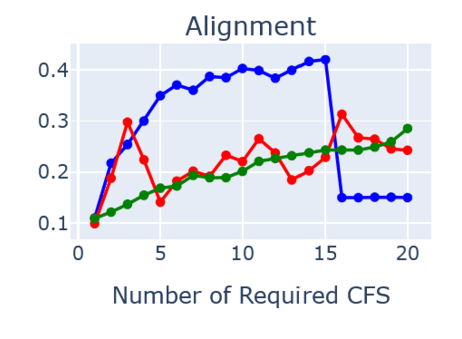
\includegraphics[width=\textwidth]{images/alignment-adult-1.png}
    \caption{adult dataset.}
    \label{fig:image1}
  \end{subfigure}
  \hfill
  \begin{subfigure}{0.45\textwidth}
    \centering
    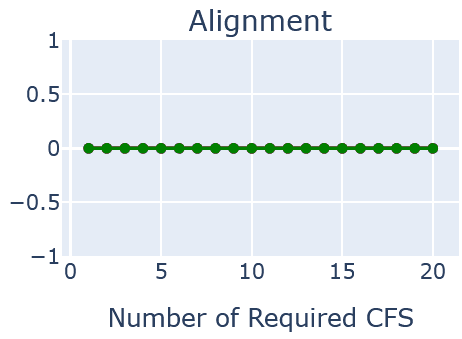
\includegraphics[width=\textwidth]{images/alignment-german_credit-1.png}
    \caption{german\_credit dataset.}
    \label{fig:image2}
  \end{subfigure}
  
  \vspace{0.5cm} 

  \begin{subfigure}{0.45\textwidth}
    \centering
    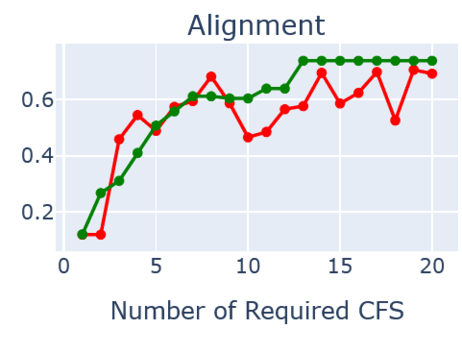
\includegraphics[width=\textwidth]{images/alignment-compas-1.png}
    \caption{compas dataset.}
    \label{fig:image3}
  \end{subfigure}
  \hfill
  \begin{subfigure}{0.45\textwidth}
    \centering
    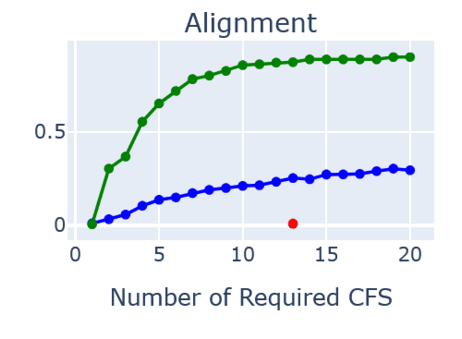
\includegraphics[width=\textwidth]{images/alignment-fico-1.png}
    \caption{fico dataset.}
    \label{fig:image4}
  \end{subfigure}
  
  \caption{Image of the Alignment metric for the explainers on the datasets, varying the required number of required counterfactuals. There seems to be the same issue as observed in Actionability with complex feature names in german\_credit.}
  \label{fig:four_image_grid}
\end{figure}
\chapter{Conclusion\label{chap:conclusion}}
\section{Summary}
This dissertation aimed to evaluate and statistically compare the performance of three counterfactual explanation generation frameworks, DiCE and AIDE, with an additional evaluation of DiCE's genetic variant based on GeCo. The study addressed the research questions of whether AIDE, an immune-inspired algorithm, is well-suited for counterfactual generation compared to DiCE and DiCE-genetic. To achieve this, a comprehensive experiment was conducted, employing both quantitative evaluation using established metrics (Size, Dissimilarity, Actionability, Diversity, and Runtime) and qualitative analysis through parallel coordinates plots across four benchmark tabular datasets.

The quantitative results revealed that both AIDE and DiCE generally achieved the requested size of counterfactuals, while DiCE-genetic struggled to consistently do so. In terms of the key metrics in the literature, DiCE demonstrated the best proximity to the original instance (lowest dissimilarity distance), with statistically significant differences compared to AIDE and DiCE-genetic. On the other hand, AIDE exhibited higher diversity in both distance and count, significantly outperforming the other methods in diversity count. The difference in means for the distances shows that AIDE possibly handles the trade-off better than the other methods. AIDE showed a tendency for higher actionability, although this was not statistically significant overall. Regarding computational efficiency, DiCE-genetic had the fastest runtime, followed by DiCE, while AIDE was significantly slower due to the experimental setup involving a higher iteration limit and a single-shot generation approach.

The qualitative analysis using parallel coordinates plots provided valuable insights into how each method alters features to generate counterfactuals. These visualizations suggested that the methods handle continuous and categorical features differently, highlighting potential limitations in how each framework explores the feature space and adheres to the underlying data distribution. For example, DiCE sometimes generated counterfactuals in low-density regions of the data, and struggled with changing categorical features in the adult dataset. AIDE generally performed well with categorical features but occasionally produced unrealistic combinations.

Overall, the findings suggest that no single method is definitively superior across all evaluation metrics. This agrees with work by \citet{guidotti2024counterfactual}. While AIDE performed well in terms of diversity and showed promise in actionability, it suffered from longer runtimes and higher dissimilarity distances compared to DiCE in some cases. DiCE excelled in generating proximal counterfactuals but sometimes lacked diversity and struggled with categorical features. DiCE-genetic offered faster runtimes but had issues with consistently generating the required number of valid counterfactuals. Therefore due to the high variance across all of the datasets, the choice of the most suitable counterfactual explanation method depends on the specific application and the dataset. When building a counterfactual-based XAI system, the three methods or maybe even more could be used to generate CFs. As it is already known by \citet{miller2019explanation} good explanations are also selective. So the next step would be to figure out the relative importance of different evaluation criteria for an end user.

\section{Future Work}
This work points towards several areas for future investigation. First of all, concerning the metrics. Other metrics like Instability, Implausibility, and Discriminative Power in section \ref{subsection:metrics} can be measured among DiCE, DiCE-genetic and AIDE. Another important check can be done by measuring the metrics separately for categorical and continuous features. Perhaps some explainers handle this better than others since it is a challenging task to quantify the amount of "difficulty" to change a categorical value to another one. Moreover, the proposed "Alignment" metric could be evaluated among all of the methods discussed in \citet{guidotti2024counterfactual}.

AIDE can be further improved by exploring adaptive strategies for hyperparameter tuning in AIDE, particularly the affinity constant. This could potentially a greater optimization to the trade-off between Diversity and Disimilarity, and possibly reduce the runtime. AIDE could also be adapted to hybrid approach and have diversity baked into the method. It could optimize equation \ref{eq:dice-loss} and the term $dpp\_diversity$ could prove to be very advantageous to find counterfactuals.

Extending the benchmarking to a wider range of datasets, including those with different characteristics (e.g., higher dimensionality, imbalanced classes), would provide a more robust comparison of the methods' generalizability. Perhaps a comparison between domains/datasets could be done to see if counterfactuals perform better in some domains/datasets than others.

There is a lack of user studies to evaluate the discriminative power and "loveliness" of the counterfactual explanations. Experiments similar to \citet{forrest2021contrastive} can be done to include DiCE-genetic to provide crucial insights into their practical utility and user satisfaction.


To conclude, this comparative analysis not only reaffirms the complexity of generating truly effective counterfactual explanations, a significant challenge of making inherently opaque 'black box' models understandable, but also highlights the nuanced trade-offs between key properties like diversity and proximity. While no single method emerged as universally superior, the insights about the distinct behaviors of explainers on different feature types and the introduction of the Alignment metric direct the way for future hybrid approaches and user-centered evaluations. These advancements are essential for advancing the frontier of XAI toward systems that are not just interpretable, but genuinely trustworthy and beneficial in critical and socially sensitive decision-making contexts.
% Seperate Categorical and Continuous Features
% Suggest new algorithim - AIDE with DPP
%\begin{enumerate}
%\item Measure metrics like Instability, Implausibility, and Discriminative Power.
%\item Develop a version of AIDE that is optimized for a certain metric.
%\item Compare counterfactuals from different domains to check if counterfactuals perform better in some domains than others.
%\item Compare counterfactuals from different Black Box Models to see if counterfactuals perform better in specific models.
%\end{enumerate}

\bibliography{mybib}
\appendix
\chapter{User Manual\label{chap:user-manual}}
\lstset{style=mystyle}
\section{Prerequisites}
\begin{itemize}
    \item Python 3.11.11
\end{itemize}

\section{Installation}
\subsection{Step 1: Clone or Unzip the Repository}
Clone the repository or unzip the \texttt{counterfactual\_explainers-main.zip} file.
\begin{lstlisting}[style=shell]
git clone https://github.com/Hariss-Gills/counterfactual_explainers.git
\end{lstlisting}

\subsection{Step 2: Create Virtual Environments}
Create virtual environments for each counterfactual method.
\begin{lstlisting}[style=shell]
python -m venv ~/.python-venvs/counterfactual-explainers-dice
python -m venv ~/.python-venvs/counterfactual-explainers-aide
\end{lstlisting}

\subsection{Step 3: Install Required Packages}
Install the necessary packages for each method.
\begin{lstlisting}[style=shell]
cd counterfactual_explainers

source ~/.python-venvs/counterfactual-explainers-dice/bin/activate
pip install .
pip install -r requirements-dice.txt
deactivate

source ~/.python-venvs/counterfactual-explainers-aide/bin/activate
pip install .
pip install -r requirements-aide.txt
deactivate
\end{lstlisting}

\section{Usage}
Run the top level modules using the respective virtual environments.
\begin{lstlisting}[style=shell]
source ~/.python-venvs/counterfactual-explainers-dice/bin/activate
python counterfactual_explainers/dataset_stats.py
python counterfactual_explainers/train_models.py
python counterfactual_explainers/gen_cfs_dice.py
deactivate

source ~/.python-venvs/counterfactual-explainers-aide/bin/activate
python counterfactual_explainers/gen_cfs_aide.py
python counterfactual_explainers/calculate_metrics.py
python counterfactual_explainers/plot_and_stats.py
deactivate
\end{lstlisting}

\section{Notes}
\begin{itemize}
    \item It is necessary to downgrade from Python 3.13.1 to 3.12.8 due to TensorFlow compatibility.
    \item TensorFlow must be downgraded to \texttt{tensorflow==2.13.0} since \texttt{dice\_ml==0.11} uses that version. Downgrading scikit-learn might also resolve the deserialization issue between using the pipeline versus a raw model.
    \item Since \href{https://github.com/scikit-learn/scikit-learn/blob/d666202a9349893c1bd106cc9ee0ff0a807c7cf3/sklearn/base.py#L540}{\texttt{ClassifierMixin}} does not have a superclass, the \texttt{Tags()} class is used to instantiate some tags instead of downgrading scikit-learn.
\end{itemize}
\chapter{Maintenance Manual\label{chap:maintenance-manual}}

More API docs are available in the \inlinecode{counterfactual\_explainers/docs} directory.  

\section{\inlinecode{counterfactual\_explainers.dataset\_stats}}
\label{sec:dataset_stats}
A module for generating dataset statistics and preprocessing pipeline metrics.

This module provides functionality to analyze datasets and their preprocessing
pipelines, calculating key metrics about feature types, encoding results, and
label distributions. Results are exported to CSV for easy reporting.

\paragraph{Key functions:}
\begin{itemize}
    \item \inlinecode{get\_pipeline\_stats}: Calculates preprocessing pipeline metrics for a dataset.
    \item \inlinecode{main}: Main execution flow that processes all configured datasets.
\end{itemize}

\subsection{\inlinecode{get\_pipeline\_stats()}}
\label{func:get_pipeline_stats}

\begin{lstlisting}
counterfactual_explainers.dataset_stats.get_pipeline_stats(data: DatasetDict) -> dict[str, int | None]
\end{lstlisting}

Analyzes a dataset and its preprocessing pipeline to calculate key metrics.

\begin{description}
    \item[Parameters:]
        \begin{itemize}
            \item \inlinecode{data}: Dataset dictionary containing features, target, and metadata from \inlinecode{read\_dataset}. Must include:
                \begin{itemize}
                    \item \inlinecode{continuous\_features}: List of continuous feature names
                    \item \inlinecode{categorical\_features}: List of categorical feature names
                    \item \inlinecode{features}: Full feature DataFrame
                    \item \inlinecode{target}: Target variable Series
                    \item \inlinecode{non\_act\_features}: List of non-actionable feature names
                    \item \inlinecode{encode}: Encoding strategy used for categorical features
                    \item \inlinecode{scaler}: Scaling strategy used for continuous features
                \end{itemize}
        \end{itemize}
    \item[Returns:] Dictionary containing calculated metrics with keys:
        \begin{itemize}
            \item 'Number of Records': Total number of instances in the dataset
            \item 'Number of Features': Original number of features before encoding
            \item 'Number of Continuous Features': Count of numerical features
            \item 'Number of Categorical Features': Count of categorical features
            \item 'Number of Actionable Features': Features available for modification
            \item 'Number of Encoded Features': Resulting features after encoding
            \item 'Number of Labels': Distinct classes in the target variable
        \end{itemize}
    \item[Return type:] \inlinecode{dict}
\end{description}

\subsection{\inlinecode{main()}}
\label{func:dataset_stats_main}

\begin{lstlisting}
counterfactual_explainers.dataset_stats.main() -> None
\end{lstlisting}

Main execution function that processes all datasets in configuration. Reads and cleans configuration, processes each dataset listed in the configuration file, calculates pipeline statistics, and exports results to a CSV file in the results directory.

% --- Module: counterfactual_explainers.train_models ---
\section{\inlinecode{counterfactual\_explainers.train\_models}}
\label{sec:train_models}

A module for training and evaluating machine learning models with explainer integration.

This module provides end-to-end functionality for:
\begin{itemize}
    \item Configuring and training Random Forest and DNN models
    \item Hyperparameter tuning using RandomizedSearchCV
    \item Model evaluation with multiple metrics
    \item Integration with different explainer frameworks (AIDE/DICE)
    \item Saving trained models and results
\end{itemize}

\paragraph{Key components:}
\begin{itemize}
    \item \inlinecode{build\_dnn}: Constructs customizable neural network architectures
    \item \inlinecode{train\_model}: Handles model training with hyperparameter tuning
    \item \inlinecode{evaluate\_model}: Calculates performance metrics
    \item \inlinecode{train\_and\_evaluate\_for\_dataset}: Manages dataset-specific training workflows
    \item \inlinecode{main}: Coordinates end-to-end training process
\end{itemize}


\subsection{\inlinecode{build\_dnn()}}
\label{func:build_dnn}

\begin{lstlisting}
counterfactual_explainers.train_models.build_dnn(
    dim_0, dim_out, dim_1=128, dim_2=64, activation_0='relu',
    activation_1='relu', activation_2='relu', dropout_0=0.3,
    dropout_1=0.1, dropout_2=0.01
)
\end{lstlisting}

Construct a deep neural network architecture with configurable layers. Creates a sequential neural network with dense layers and optional dropout. The final layer uses sigmoid activation for binary classification or softmax for multi-class (automatically determined during training).

\begin{description}
    \item[Parameters:]
        \begin{itemize}
            \item \inlinecode{dim\_0}: Input dimension size (must match preprocessed feature dimension)
            \item \inlinecode{dim\_out}: Output dimension size (number of classes)
            \item \inlinecode{dim\_1}: First hidden layer size, default 128
            \item \inlinecode{dim\_2}: Second hidden layer size, default 64
            \item \inlinecode{activation\_0}: Activation for input layer, default 'relu'
            \item \inlinecode{activation\_1}: Activation for first hidden layer, default 'relu'
            \item \inlinecode{activation\_2}: Activation for second hidden layer, default 'relu'
            \item \inlinecode{dropout\_0}: Dropout rate after input layer, default 0.3
            \item \inlinecode{dropout\_1}: Dropout rate after first hidden layer, default 0.1
            \item \inlinecode{dropout\_2}: Dropout rate after second hidden layer, default 0.01
        \end{itemize}
    \item[Returns:] Uncompiled Keras Sequential model
    \item[Return type:] \inlinecode{keras.models.Sequential} % Adjust based on actual Keras import
\end{description}

\subsection{\inlinecode{evaluate\_model()}}
\label{func:evaluate_model}

\begin{lstlisting}
counterfactual_explainers.train_models.evaluate_model(
    y_true: numpy.ndarray, y_pred: numpy.ndarray
) -> dict[str, float]
\end{lstlisting}

Calculate evaluation metrics for model performance.

\begin{description}
    \item[Parameters:]
        \begin{itemize}
            \item \inlinecode{y\_true}: Ground truth labels (\inlinecode{numpy.ndarray})
            \item \inlinecode{y\_pred}: Model predictions (\inlinecode{numpy.ndarray})
        \end{itemize}
    \item[Returns:] Dictionary containing:
        \begin{itemize}
            \item \inlinecode{accuracy}: Overall accuracy
            \item \inlinecode{f1\_macro}: Macro-averaged F1 score
            \item \inlinecode{f1\_micro}: Micro-averaged F1 score
        \end{itemize}
    \item[Return type:] \inlinecode{dict}
\end{description}

\subsection{\inlinecode{parse\_arguments()}}
\label{func:parse_arguments}

\begin{lstlisting}
counterfactual_explainers.train_models.parse_arguments()
\end{lstlisting}

Parse command line arguments for explainer framework selection.

\begin{description}
    \item[Returns:] Configured argument parser with explainer type
    \item[Return type:] \inlinecode{argparse.ArgumentParser}
\end{description}

\subsection{\inlinecode{save\_model()}}
\label{func:save_model}

\begin{lstlisting}
counterfactual_explainers.train_models.save_model(
    best_pipeline: sklearn.pipeline.Pipeline, model_name: str,
    dataset_name: str, explainer_type: str
) -> pathlib.Path
\end{lstlisting}

Save trained model to disk in format appropriate for each model type.

\begin{description}
    \item[Parameters:]
        \begin{itemize}
            \item \inlinecode{best\_pipeline}: Trained scikit-learn pipeline
            \item \inlinecode{model\_name}: Type of model ('RF' or 'DNN')
            \item \inlinecode{dataset\_name}: Name of dataset used for training
            \item \inlinecode{explainer\_type}: Type of explainer ('aide' or 'dice')
        \end{itemize}
    \item[Returns:] Location where model was saved
    \item[Return type:] \inlinecode{pathlib.Path}
\end{description}

\subsection{\inlinecode{set\_random\_seeds()}}
\label{func:set_random_seeds}

\begin{lstlisting}
counterfactual_explainers.train_models.set_random_seeds(seed: int) -> None
\end{lstlisting}

Set random seeds for reproducibility across multiple libraries.
WARNING: May exhibit unexpected behavior with certain TensorFlow versions or when combined with GPU computations.

\begin{description}
    \item[Parameters:]
        \begin{itemize}
            \item \inlinecode{seed}: Integer value to seed all random number generators
        \end{itemize}
\end{description}

\subsection{\inlinecode{train\_and\_evaluate\_for\_dataset()}}
\label{func:train_and_evaluate_for_dataset}

\begin{lstlisting}
counterfactual_explainers.train_models.train_and_evaluate_for_dataset(
    dataset_name: str, config: dict[str, Any], explainer_type: str
) -> list[dict[str, Any]]
\end{lstlisting}

Orchestrate model training and evaluation for a single dataset.

\begin{description}
    \item[Parameters:]
        \begin{itemize}
            \item \inlinecode{dataset\_name}: Name of dataset to process
            \item \inlinecode{config}: Loaded configuration dictionary
            \item \inlinecode{explainer\_type}: Type of explainer framework being used
        \end{itemize}
    \item[Returns:] List of dictionaries containing training results for each model
\end{description}

\subsection{\inlinecode{train\_model()}}
\label{func:train_model}

\begin{lstlisting}
counterfactual_explainers.train_models.train_model(
    X_train: pandas.DataFrame, y_train: pandas.Series, preprocessor: Any,
    model: Any, params_model: dict[str, Any], seed: int
) -> sklearn.pipeline.Pipeline
\end{lstlisting}

Train a machine learning model with hyperparameter tuning. Constructs a scikit-learn pipeline with preprocessing and classifier, then performs randomized search for hyperparameter optimization.

\begin{description}
    \item[Parameters:]
        \begin{itemize}
            \item \inlinecode{X\_train}: Training features DataFrame
            \item \inlinecode{y\_train}: Training target Series
            \item \inlinecode{preprocessor}: Configured data preprocessing transformer
            \item \inlinecode{model}: Uninitialized classifier model
            \item \inlinecode{params\_model}: Hyperparameter search space for RandomizedSearchCV
            \item \inlinecode{seed}: Random seed for reproducibility
        \end{itemize}
    \item[Returns:] Best performing pipeline from hyperparameter search
    \item[Return type:] \inlinecode{sklearn.pipeline.Pipeline}
\end{description}


% --- Module: counterfactual_explainers.gen_cfs_aide ---
\section{\inlinecode{counterfactual\_explainers.gen\_cfs\_aide}}
\label{sec:gen_cfs_aide}

A module for generating counterfactual explanations using the AIDE framework.

This module provides functionality for:
\begin{itemize}
    \item Loading pre-trained Keras models
    \item Preparing dataset-specific configurations for AIDE
    \item Generating counterfactual explanations using artificial immune networks
    \item Handling dataset encoding/decoding for explanations
    \item Saving counterfactual results and runtime metrics
\end{itemize}

\paragraph{Key components:}
\begin{itemize}
    \item \inlinecode{generate\_and\_save\_counterfactuals}: Core AIDE explanation generation workflow
    \item \inlinecode{generate\_cfs\_for\_dataset}: Dataset-specific explanation orchestration
    \item \inlinecode{decode\_df}: Helper for decoding encoded feature representations
    \item \inlinecode{DATASET\_PARAMS}: Pre-configured parameters for different datasets
\end{itemize}


\subsection{\inlinecode{generate\_and\_save\_counterfactuals()}}
\label{func:generate_and_save_counterfactuals}

\begin{lstlisting}
counterfactual_explainers.gen_cfs_aide.generate_and_save_counterfactuals(
    model: keras.models.Model, X_test: pandas.DataFrame, index_in_arr: int,
    aide_data_object: dict[str, Any], model_name: str, dataset_name: str,
    prob_dict: dict[str, float]
) -> None
\end{lstlisting}

Generate and persist counterfactual explanations using AIDE.

\begin{description}
    \item[Parameters:]
        \begin{itemize}
            \item \inlinecode{model}: Pretrained Keras model for prediction
            \item \inlinecode{X\_test}: Test features DataFrame
            \item \inlinecode{index\_in\_arr}: Index of query instance in test set
            \item \inlinecode{aide\_data\_object}: Dataset-specific configuration dictionary
            \item \inlinecode{model\_name}: Type of ML model being explained
            \item \inlinecode{dataset\_name}: Name of dataset being used
            \item \inlinecode{prob\_dict}: Probability dictionary for target classes
        \end{itemize}
\end{description}

\subsection{\inlinecode{generate\_cfs\_for\_dataset()}}
\label{func:generate_cfs_for_dataset}

\begin{lstlisting}
counterfactual_explainers.gen_cfs_aide.generate_cfs_for_dataset(
    dataset_name: str, config: dict[str, Any]
) -> None
\end{lstlisting}

Orchestrate counterfactual generation workflow for a dataset.

\begin{description}
    \item[Parameters:]
        \begin{itemize}
            \item \inlinecode{dataset\_name}: Name of dataset to process
            \item \inlinecode{config}: Configuration dictionary with parameters
        \end{itemize}
\end{description}

\subsection{\inlinecode{main()}}
\label{func:gen_cfs_aide_main}

\begin{lstlisting}
counterfactual_explainers.gen_cfs_aide.main() -> None
\end{lstlisting}

Main execution function for AIDE counterfactual generation.


% --- Module: counterfactual_explainers.calculate_metrics ---
\section{\inlinecode{counterfactual\_explainers.calculate\_metrics}}
\label{sec:calculate_metrics}

A module for calculating counterfactual explanation metrics.

This module provides functionality for:
\begin{itemize}
    \item Computing various counterfactual quality metrics (distance, diversity, actionability)
    \item Encoding counterfactual data for metric calculation
    \item Loading pre-generated counterfactual results
    \item Generating comprehensive metric reports for different models and datasets
\end{itemize}

\paragraph{Key components:}
\begin{itemize}
    \item \inlinecode{calc\_mad}: Computes Median Absolute Deviation for continuous features
    \item \inlinecode{calc\_distance}: Calculates normalized distance between instances
    \item \inlinecode{calc\_diversity}: Measures diversity among counterfactual explanations
    \item \inlinecode{encode\_cfs\_to\_dfs}: Preprocesses data for metric calculation
    \item \inlinecode{calculate\_metrics\_for\_dataset}: Orchestrates metric calculation workflow
\end{itemize}


\subsection{\inlinecode{calc\_actionability()}}
\label{func:calc_actionability}

\begin{lstlisting}
counterfactual_explainers.calculate_metrics.calc_actionability(
    cf_row: pandas.Series, query_instance: pandas.DataFrame,
    non_act_features: list[str]
) -> int
\end{lstlisting}

Check if counterfactual makes changes to non-actionable features.

\begin{description}
    \item[Parameters:]
        \begin{itemize}
            \item \inlinecode{cf\_row}: Counterfactual instance as pandas Series
            \item \inlinecode{query\_instance}: Original query instance as DataFrame
            \item \inlinecode{non\_act\_features}: List of non-actionable feature names
        \end{itemize}
    \item[Returns:] 1 if no changes to non-actionable features, 0 otherwise
\end{description}

\subsection{\inlinecode{calc\_changes()}}
\label{func:calc_changes}

\begin{lstlisting}
counterfactual_explainers.calculate_metrics.calc_changes(
    cf_row: pandas.Series, query_instance: pandas.Series,
    features: list[str]
) -> int
\end{lstlisting}

Count number of feature changes between counterfactual and query instance.

\begin{description}
    \item[Parameters:]
        \begin{itemize}
            \item \inlinecode{cf\_row}: Counterfactual instance as pandas Series
            \item \inlinecode{query\_instance}: Original query instance as pandas Series
            \item \inlinecode{features}: List of feature names to consider
        \end{itemize}
    \item[Returns:] Number of changed features as integer
\end{description}


\subsection{\inlinecode{calc\_distance()}}
\label{func:calc_distance}

\begin{lstlisting}[language=Python, caption={Function Signature}]
counterfactual_explainers.calculate_metrics.calc_distance(
    cf_row: pandas.Series, query_instance: pandas.Series, mad: pandas.Series,
    continuous_features: list[str], categorical_features: list[str]
) -> float
\end{lstlisting}

Calculate normalized distance between counterfactual and query instance.

\begin{description}
    \item[Parameters:]
        \begin{itemize}
            \item \inlinecode{cf\_row}: Counterfactual instance as pandas Series
            \item \inlinecode{query\_instance}: Original query instance as pandas Series
            \item \inlinecode{mad}: MAD values for continuous features (as pandas Series)
            \item \inlinecode{continuous\_features}: List of continuous feature names
            \item \inlinecode{categorical\_features}: List of categorical feature names
        \end{itemize}
    \item[Returns:] Combined normalized distance (continuous + categorical) as float
    \item[Return type:] \inlinecode{float}
\end{description}


\subsection{\inlinecode{calc\_diversity()}}
\label{func:calc_diversity}

\begin{lstlisting}[language=Python, caption={Function Signature}]
counterfactual_explainers.calculate_metrics.calc_diversity(
    cfs: pandas.DataFrame, continuous_features: list[str],
    categorical_features: list[str], feature_cols: list[str],
    mad: pandas.Series
) -> tuple[float, float]
\end{lstlisting}

Calculate diversity metrics for a set of counterfactuals.

\begin{description}
    \item[Parameters:]
        \begin{itemize}
            \item \inlinecode{cfs}: DataFrame of counterfactual instances
            \item \inlinecode{continuous\_features}: List of continuous feature names
            \item \inlinecode{categorical\_features}: List of categorical feature names
            \item \inlinecode{feature\_cols}: All feature names
            \item \inlinecode{mad}: MAD values for continuous features (as pandas Series)
        \end{itemize}
    \item[Returns:] Tuple containing:
        \begin{itemize}
            \item \inlinecode{diversity\_distance}: Normalized pairwise distance metric
            \item \inlinecode{diversity\_count}: Normalized feature change count metric
        \end{itemize}
    \item[Return type:] \inlinecode{tuple}
\end{description}


\subsection{\inlinecode{calc\_mad()}}
\label{func:calc_mad}

\begin{lstlisting}[language=Python, caption={Function Signature}]
counterfactual_explainers.calculate_metrics.calc_mad(cf_row: pandas.Series) -> float
\end{lstlisting}

Calculate Median Absolute Deviation (MAD) for a given data row.

\begin{description}
    \item[Parameters:]
        \begin{itemize}
            \item \inlinecode{cf\_row}: Pandas Series representing a single data row
        \end{itemize}
    \item[Returns:] MAD value as float. Returns 1.0 if MAD is zero to avoid division by zero.
    \item[Return type:] \inlinecode{float}
\end{description}


\subsection{\inlinecode{calc\_range\_alignment()}}
\label{func:calc_range_alignment}

\begin{lstlisting}[language=Python, caption={Function Signature}]
counterfactual_explainers.calculate_metrics.calc_range_alignment(
    cfs_df: pandas.DataFrame, target_class_instances: pandas.DataFrame,
    continuous_features: list[str], categorical_features: list[str]
) -> float
\end{lstlisting}

Calculates the alignment between the value ranges of counterfactuals and the value ranges of actual instances belonging to the target class.

For continuous features, it uses a discretization approach over the union range, then computes the Jaccard index using scipy. For categorical features, it creates binary indicator arrays for the sets of unique values and computes the Jaccard index using scipy.

The scores are printed directly for each feature. % Note: Original text mentions printing; the function might do more than just return a single float.

\begin{description}
    \item[Parameters:]
        \begin{itemize}
            \item \inlinecode{cfs\_df}: DataFrame of counterfactual instances (original, unencoded values).
            \item \inlinecode{target\_class\_instances}: DataFrame containing only instances from the original dataset belonging to the target class (original, unencoded values).
            \item \inlinecode{continuous\_features}: List of continuous feature names.
            \item \inlinecode{categorical\_features}: List of categorical feature names.
        \end{itemize}
     % Note: No explicit 'Returns' block in the Sphinx source, but signature indicates float.
     \item[Return type:] \inlinecode{float} % Based on signature, represents overall alignment perhaps?
\end{description}


\subsection{\inlinecode{calc\_size()}}
\label{func:calc_size}

\begin{lstlisting}[language=Python, caption={Function Signature}]
counterfactual_explainers.calculate_metrics.calc_size(
    num_required_cfs: int, cfs_df: pandas.DataFrame
) -> float
\end{lstlisting}

Calculate size metric as ratio of generated CFs to required CFs.

\begin{description}
    \item[Parameters:]
        \begin{itemize}
            \item \inlinecode{num\_required\_cfs}: Requested number of counterfactuals
            \item \inlinecode{cfs\_df}: DataFrame containing generated counterfactuals
        \end{itemize}
    \item[Returns:] Size metric as float
    \item[Return type:] \inlinecode{float}
\end{description}


\subsection{\inlinecode{calculate\_metrics\_for\_dataset()}}
\label{func:calculate_metrics_for_dataset}

\begin{lstlisting}[language=Python, caption={Function Signature}]
counterfactual_explainers.calculate_metrics.calculate_metrics_for_dataset(
    config: dict[str, Any], dataset: str
) -> None
\end{lstlisting}

Calculate metrics for a dataset across models and explainers.

\begin{description}
    \item[Parameters:]
        \begin{itemize}
            \item \inlinecode{config}: Configuration dictionary
            \item \inlinecode{dataset}: Dataset name to process
        \end{itemize}
\end{description}


\end{document}
